\documentclass{article} % Loads settings for the document layout

\usepackage[utf8]{inputenc}
\usepackage[T1]{fontenc}
\usepackage{currvita}
\usepackage{graphicx}
\usepackage{float} % podrska za float smestanje figura <=> opcija [H]
\usepackage{latexsym} % podrska za specijalne simbole
\graphicspath{ {images/} }
\title{Mrežno računarstvo - skripta}


% Main document

\begin{document} % The document starts here

\maketitle % Creates the titlepage
\pagenumbering{gobble} % Turns off page numbering
\newpage % Starts a new page
\pagenumbering{arabic} % Turns on page numbering

\section{Komponente mreže, tipovi veza, primeri mreža, mreže prema dimenziji, međumreže}
(preuzeto sa slajdova)
\subsection{Komponente mreže}
Delovi mreže su:\\ 
- \textit{aplikacija}, odnosno korisnik čija je funkcija da koristi mrežu. Primeri za aplikaciju su Skype, iTunes, Amazon.\\
- \textit{računar} ili završni čvor, izvor, uređaj čija je funkcija da podržava aplikaciju. Primeri su laptop, mobilni telefon..\\
- \textit{ruter} ili usmerivač, tj. središnji čvor čija je funkcija da prosleđuje poruke između  čvorova. Primeru su pristupna tačka, kablovski/DSL modem..\\
- \textit{veza} ili kanal čija je funkcija da spaja čvorove. Primeri su žičane veze i bežične veze.
\subsection{Tipovi veza}
Tipovi veza koji postoje: \\
- \textit{simpleks} (u jednom smeru).\\
Simpleks transmisija dozvoljava komunikaciju samo u jednom smeru. Emitovanje televizijskih i radio signala je primer ovakve vrste transmisije. Kako komunikacija obično zahteva povratnu informaciju, ovaj tip veze se retko koristi za prenos podataka. \\
-\textit{poludupleks}(u oba smera) \\
Polu-dupleks transmisija dozvoljava komunikaciju u oba smera ali ne u istom trenutku. Tipičan primer je radio-veza: dok jedna strana govori, druga ne može da odgovori dok poruka ne bude završena. Ovakva veza među računarima se obično koristi za paketnu transmisiju podataka. \\
- \textit{puni dupleks} (u oba smera istovremeno)\\
Puna dupleks transmisija dozvoljava simultanu komunikaciju u oba smera. Tipičan
primer je telefonska veza. Među računarima se ova veza prvenstveno koristi za interaktivni ulaz i procesiranje u realnom vremenu.\\

\subsection{Primeri mreža}
Primeri mreža su: WiFi (802.11), poslovne/Ethernet, ISP(Internet Service Provider), kablovska/ DSL, mobilna telefonija (2G, 3G, 4G), Bluetooth, telefon, sateliti.. 
\subsection{Mreže prema dimenziji}
Mreže prema dimenziji se dele na: \\
- \textbf{PAN} (Personal Area Network) \\
Ovo su lične mreže, namenjene jednoj osobi. Dimenzija je neposredna blizina. Primer je Bluetooth, bežična mreža koja povezuje računar s mišem, tastaturom.. \\
- \textbf{LAN} (Local Area Network)\\
Ovo su privatne mreže unutar jedne zgrade. Široko se koriste radi povezivanja ličnih računara i radnih stanica u kancelarijama firmi radi zajedničkog korišćenja resursa, npr. štampača, i razmene informacija. Ograničene su veličine pa je vreme prenosa informacija u najgorem slučaju takođe ograničeno i unapred poznato. U ovim mrežama prenos podataka se može ostvariti pomoću kabla za koji su priključeni svi računari. Brzina prenosa se kreće od 10 Mb/s do 100 Mb/s. Kašnjenje je malo, meri se mikro ili nano sekundama. Greške su retke. Nove lokalne mreže rade brzinama i do 10 Gb/s. 
Primeri su WiFi, Ethernet. Ethernet je mreža s topologijom magistrale, neusmerenim emitovanjem  i decentralizovanim upravljanjem (ne postoji jedinstvena jedinica za odlučivanje koja određuje redosled pristupanja računara magistrali, tj. svaki računar mora sam odlučiti da li će da emituje) koja obično radi brzinom između 10 Mb/s i 10 Gb/s. Računari na Ethernetu mogu da emituju poruke kad god požele; ako se dva paketa sukobe, svaki računar pauzira tokom nasumično izabranog perioda, a onda pokušava ponovo da emituje.\\
- \textbf{MAN} (Metropolitan Area Network) \\
Kako joj ime kaže, pokriva gradsko područje. Primeri su mreža kablovske televizije (TV signal se dovodi do centralnog razdvodnika odakle se dalje distribuira do kuća korisnika), DSL. \\
- \textbf{WAN} (Wide Area Network) \\
Mreža širokog područja i pokriva veliko geografsko područje, često čitavu državu ili čak kontinent. Ona sadrži skup računara namenjenih za izvršavanje korisničkih programa, tj. aplikacija. Umreženi računari su povezani komunikacionom podmrežom. Računari su vlasništvo korisnika dok je podmreža najčešće vlasništvo telefonske kompanije ili davaoca Internet usluga; oni je i održavaju. Zadatak podmreže je da prenosi poruke od jednog do drugog računara. Podmreža se sastoji od prenosnih linija i prekidačkih elemenata. Linije prenosa propuštaju bitove od jednog računara ka drugom. One mogu biti bakarne žice, optička vlakna ili radio-veza. Prekidački elementi su specijalizovani računari koji spajaju tri ili više linija prenosa. Kada podaci stignu jednom linijom, prekidački element mora da odluči kojom linijom da ih dalje uputi. Ovi prekidački računari se nazivaju \textit{usmerivači}, ili u našem računarskom žargonu \textit{ruteri}. Ako dva usmerivača koji nisu povezani istom linijom prenosa žele da komuniciraju, moraju da urade to posredno, preko drugih usmerivača.
Primer je veliki ISP (Internet Service Provider), npr. Telekom, SBB. \\
- \textbf{Internet} (mreža svih mreža) \\
Dimenzija je planeta. Primer je Internet.

\subsection{Međumreže}
Međumreža ili internet se dobija povezivanjem više različitih mreža.
Internet (sa velikim početnim slovom) je internet, tj. međumreža koji svi koristimo.\\
Mreže se povezuju pomoću uređaja zvanih mrežni prolazi (gateways) koji fizički povezuju i istovremeno usaglašavaju različite hardverske i softverske komponente dve mreže. Čest oblik međumreže jeste WAN koji povezuje više LAN-ova. U slučaju kada više organizacija investira u izgradnju različitih delova mreže i svaka održava svoj deo, iskustveno pravilo kaže da je to međumreža, a ne jedinstvena mreža. Isto tako, ako se u različitim delovima mreže koriste različite tehnologije(npr. difuzno emitovanje i prenos od tačke do tačke), verovatno se ne radi o jednoj, već o više međusobno povezanih mreža.

\subsection{Dodatak: podela mreža prema tehnologiji prenosa podataka}
Mreže sa nesumerenim emitovanjem imaju jedinstven komunikacioni kanala koji dele svi umreženi računari. Sistemi  za \textit{neusmereno(difuzno)} emitovanje najčešće imaju mogućnost da pakete usmere na sva odredišta pomoću specijalnog koda u adresnom polju. Neki takvi sistemi podržavaju i usmeravanje paketa samo na određeni podskup računara, što se naziva   \textit{višesmerno} emitovanje. Jedna mogućnost je da se u adresnom polju rezerviše jedan bit za označavanje višesmernog emitovanja. Preostalih n-1 bitova adrese mogu da sadrže broj grupe. Svaki računar može da se uključi u jednu ili više grupa. \\
Mreže od tačke do tačke (point-to-point networks) sadrže brojne veze između pojedinih parova računara. Da bi od polazišta stigao do odredišta, paket na ovom tipu mreže možda mora da prođe kroz jedan ili više drugih računara. Pronalaženje optimalne putanje je važna stavka u mrežama ovog tipa. Prenos poruka od tačke do tačke često se naziva jednosmerno emitovanje.
\section{Protokoli i slojevi}
Šta sve mreža radi za aplikacije? \\
Pravi i prekida konekciju, pronalazi putanju za transfer podataka, pouzdano šalje podatke, brzina slanja se prilagođava mogućnostima mreže, deli protok među korisnicima, omogućava novo dodavanje računara i uređaja. \\
Da bi sve ovo radila, neke stvari se moraju razdvojiti, odnosno mreži je potrebna modularnost. \\
 \textit{Protokoli i slojevi} su glavni mehanizam struktuiranja koji mreži daje modularnost. Da bi projektovanje bilo jednostavnije, mreže su većinom organizuju kao skup slojeva. Broj slojeva, njihova imena i funkcija se razlikuju od mreže do mreže.  Niži slojevi nude funkcionalnosti višim slojevima. Ovaj koncept se naziva enkapsulacija podataka.\\
Protokol predstavlja dogovor između dve jedinke o tome kako treba da teče njihova međusobna komunikacija. Protokol definiše spisak komandi koje jedna strana može da očekuje od druge i obrnuto. Svaki sloj definiše svoje zasebne protokole, a realna komunikacija se odvija samo na najnižem sloju, tj. svaka instanca protokola komunicira virtuelno sa svojim parnjakom (peer) upotrebom dogovorenih metoda, a u  stvarnosti, oni ne komuniciraju direktno, već svaka instanca koristi usluge (services) sloja koji je ispod sve dok se ne dostigne najniži sloj. Ispod sloja 1 je fizički medijum kroz koji se stvarno odvija komunikacija.   \\
Između svaka dva susedna sloja nalazi se interfejs. On određuje osnovne operacije i usluge koje donji sloj nudi gornjem. Odatle sledi da svaki sloj mora da izvršava određen skup funkcija s tačno definisanom namenom.\\
Skup slojeva i protokola se naziva jednim imenom \textbf{arhitektura mreže}.\\
Spisak protkola koji se koriste u komunikaciji se naziva \textit{protokol stek}. Na primer skup protokola koji koristi Internet pregledač na računaru koji je putem WiFi povezan na Internet: HTTP protokol se obraća nižem protokolu, tj. TCP-u, a TCP se obraća IP-u, a IP se obraća 802.11 protokolu. \\
Protokoli su horizontalni, slojevi vertikalni. \\
\begin{center}
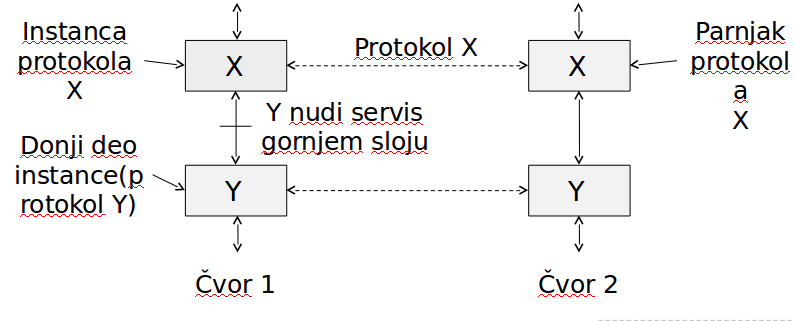
\includegraphics[width=9cm, height=5cm]{protokoli}\\
\end{center}

\subsection{Enkapsulacija}
Enkapsulacija je mehanizam slaganja slojeva protokola. Niži sloj pravi omotač oko sadržaja višeg sloja i dodaje svoje sopstvene informacije poruci. Sadržaj nižih slojeva je bliži spoljašnosti poruke. \\
\begin{center}
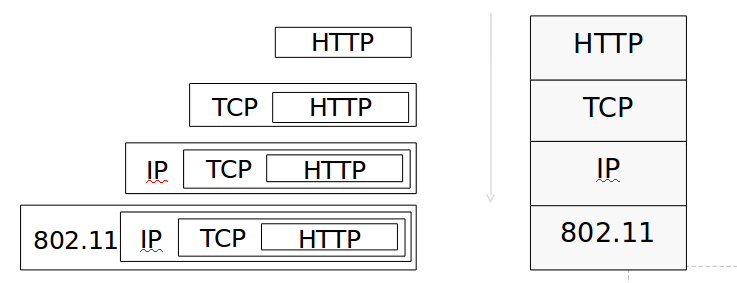
\includegraphics[width=9cm, height=4cm]{enkapsulacija}\\
\end{center}
Zahtev koji HTTP protokol definiše šalje se nižem sloju. TCP protokol dodaje svoja zaglavlja i skup informacija (metainf.) postaje sve veći kako se spuštamo po slojevima (to su enkapsulirane informacije). Zaglavlje sadrži upravljačke podatke, npr. zaglavlje jednog sloja može da sadrži redne brojeve koji omugućavaju tom istom sloju na drugom računaru da poruke isporuči ispravnim redosledom, za slučaj da niži slojevi taj redosled ne poštuju. Mogu da sadrže i veličine, vremena i druga polja. Sa svim tim informacijama se na poslednjem sloju poruka šalje na drugu stranu. Sad se informacije otpakuju, tj. primenjuje se inverzna funkcija za svaki od slojeva (uklanja se zaglavlje za svaki od slojeva) i kad se stigne do HTTP-a, on rekonstruiše originalnu poruku. \\
Smer toka podataka: $ \downarrow $(spušta se niz slojeve), zatim $ \rightarrow $
(prenosi se na najnižem sloju), pa $ \uparrow $ (podiže se uz slojeve).
\\
Protokol stek mora da bude poznat drugoj strani da bi bilo poznato kako treba da se otpakuje i svaki protokol zna samo svoju inverznu funkciju. Na drugoj strani, kada se poruka otpakuje, eliminišu se zaglavlja na svakom od slojeva i to se zove davanje usluge višim slojevima.\\
 Kada je nepogodno ili skupo da se za svaki par proces koji međusobno komuniciraju uspostavlja zasebna veza, odgovarajući sloj može da istu vezu upotrebi za više istovremenih, nezavisnih konverzacija. Sve dok je ovo \textit{multipleksiranje i demultipleksiranje} nevidljivo, može ga koristiti svaki sloj. Multipleksiranje je neophodno u fizičkom sloju gde se saobraćaj za sve veze mora preneti preko najviše nekoliko fizičkih linija. (kod njega na slajdovima stoji nešto za demultipleksiranje!)
 \\
\subsection{Prednosti raslojavanja}
- Prikrivanje informacija i ponovna upotreba\\
- Povezivanje različitih sistema\\
Šta se dešava ako imamo različite protokole na jednoj i na drugoj strani? Primer je slanje poruke sa uređaja zakačenog na WiFi na uređaj zakačenn na Ethernet. Tada na najnižim slojevima postoje tablice preslikavanja protokola. Poruka se samo prepakuje na poslednjem nivou. \\
\subsection{Mane raslojavanja}
- Povećani troškovi memorije i obrade (overhead)\\
Košta nas da dodajemo metapodatke. Manje bitno za duže poruke jer ne moramo svaki paket da dekorišemo. Početni i poslednji paket imaju veći broj informacija od središnjih, ali svaki paket ima dovoljno informacija da stigne na drugu stranu. Ne mora da budu početni i poslednji paket paketi koji imaju više informacija, mogu to biti i neki specijalni paketi. \\
- Prikrivanje informacija\\
Generalno je korisno, ali neke aplikacije žele da znaju da li se informacije prenose bežično ili putem kabla.


\section{Referentni modeli protokola i slojeva, jedince podataka, organizacije za standarde}
Ključno pitanje dizajna modela jeste koje funkcionalnosti implementira svaki od slojeva i koliko slojeva treba da postoji. Referentni modeli odgovaraju na ovakva pitanja. 
\subsection{OSI model sa 7 slojeva}

Internacionalan standard za povezivanje sistema. Uticajan ne, ali ne previše korišćen u praksi.
\\\\
1. \textbf{Fizički sloj}\\
Ima ulogu slanja \textit{bitova} putem realnih fizičkih komunikacionih kanala. U probleme njegovog projektovanja spada obezbeđivanje da kada jedna strana pošalje bit 1, druga strana takođe primi bit 1, a ne bit 0.\\\\
2. \textbf{Sloj veze podataka}\\
Ima ulogu slanja \textit{okvira}, odnosno skupova podataka. Pošiljalac ulazne podatke deli na okvire podataka, najčešće od po nekoliko stotina do nekoliko hiljada bajtova i okvire šalje jedan za drugim. Ako je usluga pouzdana, primalac potvrđuje ispravan prijem svakog okvira šaljući pošiljaocu okvir za potvrdu.
Jedan od problema koji se javlja u ovom sloju jeste neusaglašenost brzine slanja i brzine primanja podataka.\\\\
3. \textbf{Mrežni sloj}\\
Ima ulogu adresiranja, rutiranja \textit{paketa} i kontrole saobraćaja. Pri njegovom projektovanju ključno je odrediti kako se paketi upućuju od izvora ka odredištu. Putanje se mogu zasnivati na statičnim tabelama koje su ugrađene u mrežu i retko se menjaju. Jedan od zadataka ovog sloja je da omogući povezivanje heterogenih mreža.\\\\
4. \textbf{Transportni sloj}\\
Ima ulogu dostavljanja \textit{segmenata} (segmentacija, potrvđivanje). Osnovni zadatak je da prihvata podatke odzgo i da ih po potrebi razvrstava u manje grupe i da ih prosleđuje mrežnom sloju, obezbeđujući da svi delovi ispravno stignu na odredište. On takođe definiše usluge koje se nude sloju sesije.\\\\
5. \textbf{Sloj sesije}\\
Ima ulogu upravljanja sesijama.Omogućava korisnicima na različitim računarima da međusobno uspostave sesiju. Sesije nude različite usluge, uključujući upravljanje dijalogom, tj. vođenje računa o tome na koga je red da šalje poruke, rad sa žetonima, tj. sprečavanje učesnika da istovremeno pokrenu istu kritičnu operaciju i sinhronizovanje, tj. proveravanje dugačkog niza podataka tokom prenosa da bi se omogućilo nastavljanje od tačke prekida u slučaju pada sistema.\\\\
6. \textbf{Sloj prezentacije}\\
Ima ulogu konverzija za različite prezentacije. Bavi se sintaksom i semantikom prenetih informacija. Da bi računari koji podatke predstavljaju na različit način mogli da komuniciraju, strukture podataka koji se prenose mogu se definisati na apstraktan način i standardno kodirati u cilju prenosa. Sloj prezentacije obrađuje te apstraktne strukture podataka.\\\\
7. \textbf{Sloj aplikacije}\\
Ima funkcije potrebne korisniku, rad sa \textit{porukama}.  
\\
\\
Mana ovog modela jeste to što su  slojevi sesije i prezentacije gotovo prazni dok su sloj veze podataka i mrežni sloj prenatrpani.


\subsection{Internet referentni model}
Model sa 4 sloja, zasnovan na praksi. Sva tri gornja sloja se stapaju u jedan.
1. \textbf{Veza}\\
Ima ulogu fizičkog slanja podataka putem medijuma.Sam protokol za povezivanje s mrežom nije definisan i menja se od računara do računara i od jedne mreže do druge. \\\\
2. \textbf{Internet}\\
Ima ulogu slanja paketa putem raznorodnih mreža. Definiše Inernet protokol. Zadatak je da isporuči IP pakete tamo gde treba da stignu. Ovde je najveći problem problem usmeravanja i izbegavanja zagušenja.\\\\
3. \textbf{Transport}\\
Ima ulogu razmene podataka između čvorova. On je namenjen konverzaciji između ravnopravnih procesa na izvornom i odredišnom računaru, kao i transportni OSI sloj. Ovde su definisana dva protokola, protokol za upravljanje prenosom - TCP i protokol za korisničke datagrame - UDP. \\
TCP je pouzdan protokol sa uspostavljanjem direktne veze. Deli početni tok bajtova na zasebne poruke i svaku prosleđuje međumrežnom sloju. Prihvatni TCP proces na odredištu uređuje primljene poruke i od njih ponovo obrazuje tok bajtova. On upravlja i tokom podataka tako da brzi pošiljalac ne može da zatrpa sporog primaoca s više poruka nego što ovaj može da obradi. \\
UDP  predstavlja nepouzdan protokol bez uspostavljanja direktne veze namenjen aplikacijama koje same uređuju svoje pakete i upravljaju tokom podataka.\\\\
4. \textbf{Aplikacija}\\
Programi koji koriste usluge mreže. Sadrži sve protokole višeg nivoa - FTP za prenos datoteka, SMTP za elektronsku poštu, TELNET za virtuelni terminal koji omugućava korisniku da se sa svog računara daljinski prijavi na drugi računar i da na njemu radi, DNS za imenovanje domena, tj. za preslikavanje imena računara u njihove mrežne adrese, HTTP protokol za preuzimanje strana sa Worl Wide Weba i mnogi drugi.
\\\\
IP sloj je najtanji po pitanju broja protokola.

\begin{center}
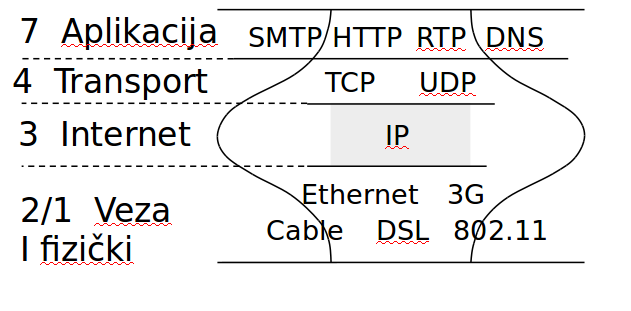
\includegraphics[width=9cm, height=4cm]{InternetRefModel}\\
\end{center}

Mana ovog modela jeste da on nije dovoljno uopšten, na primer, opisati Bluetooth pomoću ovog modela je sasvim nemoguće. Još jedna mana je to što ne razdvaja fizički sloj i sloj veze podataka. Ta dva sloja su potpuno različita. \\
\\

Mi ćemo koristiti hibridni model sa 5 slojeva: fizički sloj (bit), sloj veze (okvir), mrežni sloj (paket), transportni (segment) i aplikativni sloj (poruka). Jedinice podataka za svaki od slojeve su navedene u zagradama.\\
\\
Nazivi nekih uređaja u mreži: \\
- hab ili razvodnik ponavlja fizički signal na sve izlaze\\
- svič ili skretnica usmerava pakete samo onima kojima su potrebni, znači čita adresu\\
- ruter ili usmerivač usmerava pakete ali vodi računa i o dobrim putanjama\\\\

Neke poznatije organizacije za standarde:\\

\begin{center}
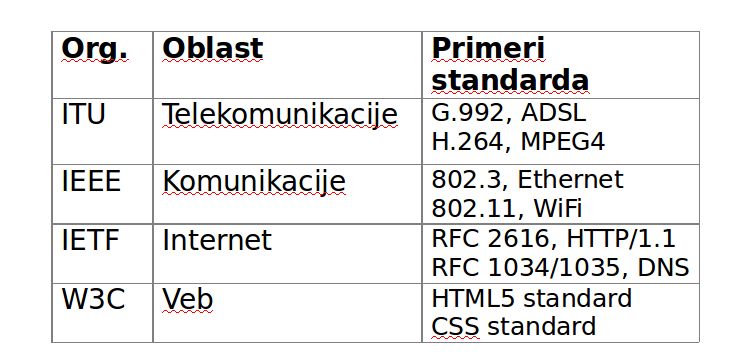
\includegraphics[width=9cm, height=4cm]{organizacije}\\
\end{center}
(Ovde kaže da treba i poglavlja 1.6 i 1.7, ali ja ne znam da li tu ima bilo šta bitno.)

\section{Fizički sloj, uloga, pojednostavljeni model, kašnjenja, BDP, primeri}
Tiče se slanja poruka putem komunikacionog kanala. Žice šalju analogni, tj. fizički signal, a mi želimo da šaljemo bitove koji su digitalni. Osnovna svrha je da niz bitova prenese bez greške s jednog računara na drugi. Za prenos mogu da se koriste različiti fizički medijumi. 
\subsection{Pojednostavljeni model}
Karakteristike uopštenog fizičkog kanala koje utiču na to koliko je kanal dobar:\\
- \textbf{\textit{protok}} (ili brzina, kapacitet) meren kao bitovi po sekundi b/s, označimo ga sa B\\
- \textbf{\textit{kašnjenje}} mereno u sekundama\\
Podrazumeva vreme potrebno da poruka stigne na ciljnu adresu. Označimo ga sa D. Postoje dve vrste kašnjenja, a to su: \\
1. \textit{Kašnjenje prenosa}, tj. vreme potrebno da se M-bitovna poruka postavi na komunikacioni kanal i različito je za sve kanale:
                 \begin{center}
                 T-delay = M (b) / B (b/s) = M/B s (sekundi)
                 \end{center}
2. \textit{Kašnjenje propagacije}, tj. vreme potrebno da bitovi prođu kroz komunikacioni kanal i slično je za sve kanale:
                  \begin{center}
           P-delay = dužina kanala/brzina signala (2/3 c) = X s (sekundi)
          *c – brzina svetlosti (nije svuda 2/3, različito za WiFi, optiku, ...)
                  \end{center}
Sabiranjem se dobija ukupno vreme.
                         \begin{center}
                         L = T+P = M/B + P
                         \end{center}
- \textbf{\textit{da li kanal emituje ili ne}}\\
- \textbf{\textit{raspodela verovatnoća grešaka}}\\
Primeri izračunavanja kašnjenja: \\
“Dialup” sa telefonskim modemom (slanje ka računaru u istom gradu npr):
                    \begin{center}
               P = 5 ms, B = 56 kb/s, M = 1250 B\\
              
               L = 5 ms + (1250x8)/(56 x 103) s = 5 ms+179 ms = 184 ms
                      \end{center}
Dugačka veza ili mali protok proizvode veće kašnjenje. Obično je jedna od komponenti kašnjenja P ili T dominantna.
\subsection{Protok-kašnjenje proizvod BDP}
BDP jeste proizvod protoka i vremena kašnjenja.
                     \begin{center}
                       BDP = B x D
                      \end{center}
Poruke zauzimaju prostor na kanalu. Količina podataka prisutnih na kanalu u nekom momentu je BDP. Ako bismo posmatrali podatak kao materiju, onda je ovo zapremina, tj. količina materije BDP = B x D. Meri se u bitovima i BDP je mali za kanale u lokalnim mrežama, npr. WiFi, a veliki za velike debele kanale.\\
\textbf{BDP primer}:\\
Slanje npr. od Perta do Sidneja preko optičkog kanala koji je dugačak.\\
B=40 Mb/s, D=50 ms $ \Rightarrow $ BDP = 40 x $10^{6}$ x 50 x $10^{-3}$ b = 2000 Kb = 250 KB\\
Ovo se smatra velikim BDP-om.\\
\\
Medijum propagira signal sa informacijama u vidu bitova. Tri osnovna tipa medija su: \\
- žičani\\
- optički (optički kablovi)\\
- bežični

\section{Žičani i optički komunikacioni medijumi}
Prednost je što se lako projektuje fiksni protok duž odabranih ruta, a mane su da je skup za postavljanje, posebno na većim udaljenostima i nije projektovan za mobilnost ili emitovanje.
\subsection{Žičani}
\subsubsection{Upredena parica}
Veoma česta, koristi se za LAN kablove i kod telefonskih linija.  Čine je dve izolovane bakarne žice, najčešće prečnika oko 1mm. Žice su međusobno spiralno uvijene, kao molekul DNK. Uvrtanjem se umanjuju smetnje. Najčešće se koristi u telefonskom sistemu, skoro svi telefoni su sa telefonskom centralom povezani uporednom paricom. Kada se veliki broj paralelnih parica protežu na veću daljinu, na primer sve linije iz jednog stambenog bloka do telefonske  centrale, one se povezuju u snop i obavijaju zaštitnim omotačem. Njome se mogu prenositi i analogni i digitalni signali. Brzina prenosa zavisi od debljine žice i rastojanja, ali se za daljine od nekoliko km u većini slučajeva može postići brzina od više megabita u sekundi.\\
Uporedna parica se realizuje u više oblika, od kojih su dva važna za računarske mreže. \\
- uporedna parica 3. kategorije se sastoji od dve blago uvijene izolovane žice. Četiri takva para obično se grupišu u zajedničkom plastičnom omotaču koji ih drži zajedno i štiti. \\
- uporedna parica 5. kategorije koje liče na parice 3. kategorije, ali su gušće upredene, čime je omogućen kvalitetniji signal na većim razdaljinama zbog čega su pogodnije za brzu komunikaciju između računara. \\
Uporedna parica 5. kategorije:
\begin{center}
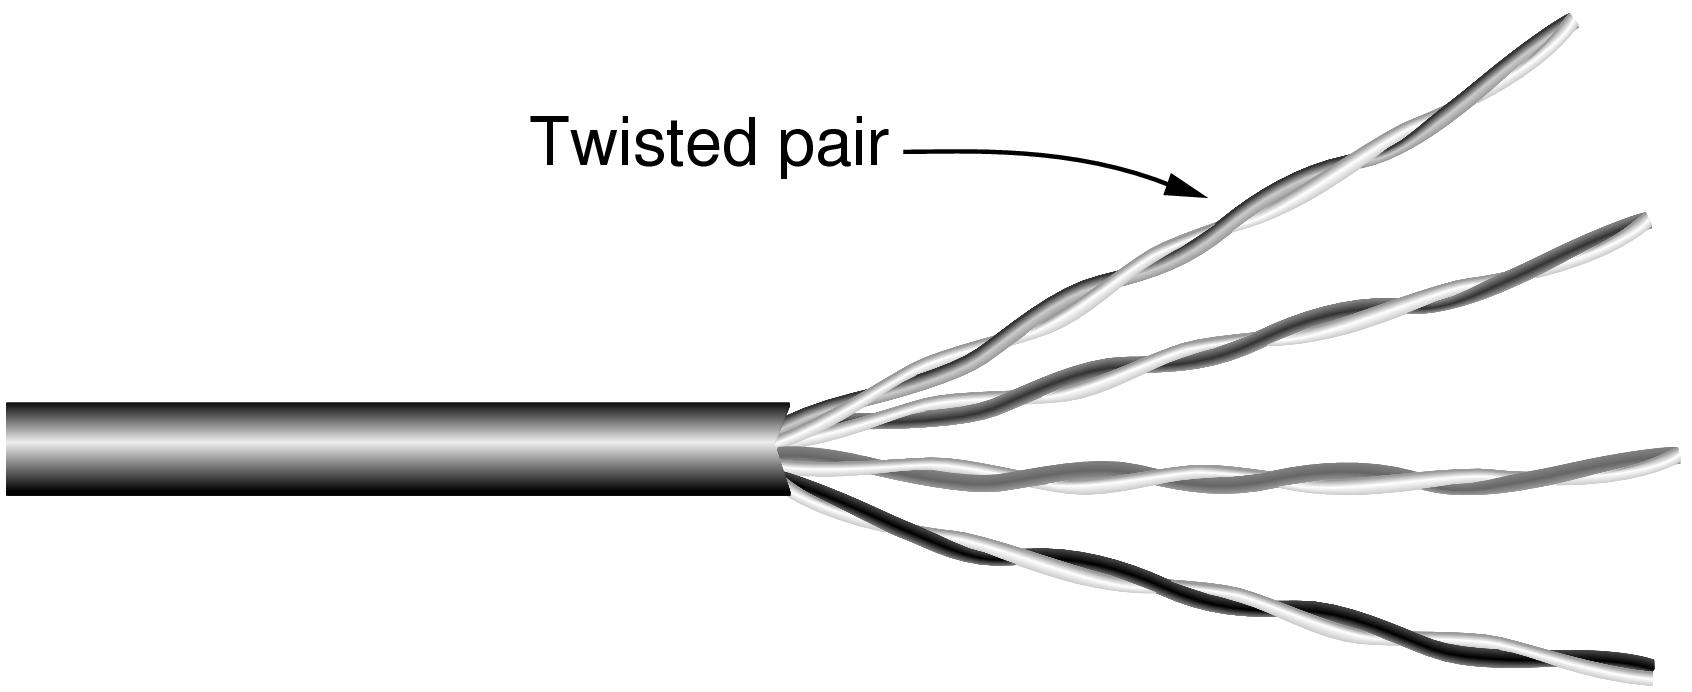
\includegraphics[width=7cm, height=3cm]{parica}\\
\end{center}

\subsubsection{Koaksijalni kabl}
Takođe čest. Daje bolju zaštitu i bolje performanse. Podatke prenosi većom brzinom i na veće daljine u odnosu na uporedne parice. Koriste se 50-omski i 75-omski koaksijalni kabl. Prvi se namenjuje digitalnom prenosu podataka, a drugi se koristi za prenos analognih podataka i za kablovsku televiziju, ali postaje sve važniji i za kablovski Internet. \\
Ovaj kabl ima jezgro od čvrste bakarne žice oko koje se nalazi izolator. Oko izolatora je cilindrični provodnik napravljen od gusto upletene bakarne mrežice. Preko njega dolazi zaštitni plastični omotač. Presek koaks. kabla:
\begin{center}
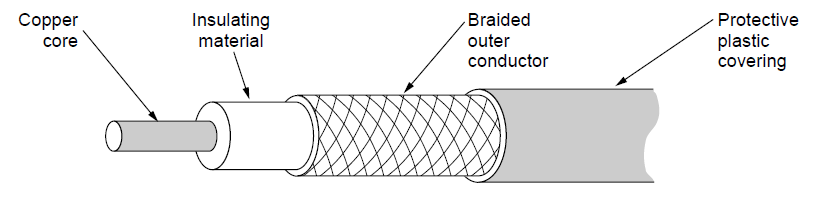
\includegraphics[width=12cm, height=3cm]{koaksijalni}\\
\end{center}
Savremeni koaks. kablovi imaju propusni opseg blizu 1GHz. Ranije su mnogo korišćeni za međugradske i međudržavne veze u telefonskim sistemima, ali su danas tu većinom zamenjeni optičkim kablovima. I dalje se koriste za kablovsku televiziju i gradske mreže.
\subsubsection{Instalacije za prenos struje}
Praktične za upotrebu jer već postoje. Jako loše karakteristike prenosa jer nisu dizajnirane za to.
\begin{center}
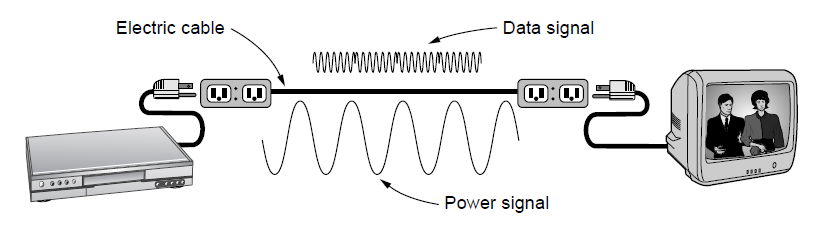
\includegraphics[width=12cm, height=3cm]{zicani}\\
\end{center}

\subsection{Optički}
Dugačka, tanka i čista vlakna stakla. Ogroman protok zbog opsega frekvencija. Velike udaljenosti zbog malog slabljenja. \\
Optički sistem za prenos podataka sadrži tri glavne komponente: svetlosni izvor, prenosni medijum i detektor. Po konvenciji, svetlosni impuls označava bit 1, a odsustvo impulsa označava bit 0. Prenosni medijum je ultratanko stakleno vlakno. Detektor proizvodi električni impuls kada na njega padne svetlosni zrak. Spajajući svetlosni izvor s jednim krajem optičkog vlakna, a detektor sa njegovim drugim krajem, dobijamo jednosmerni sistem prenosa podataka koji prihvata električni signal, pretvara ga u svetlosni impuls i prenosi, a zatim ga na drugom kraju pretvara u električni signal.
\begin{center}
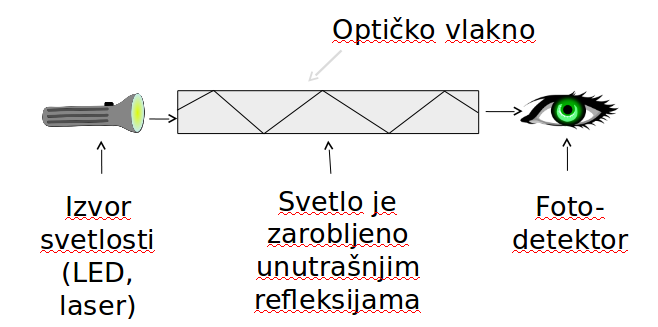
\includegraphics[width=9cm, height=4cm]{opticki1}\\
\end{center}
 Kada upadni ugao zraka pređe određenu kritičnu vrednost, zrak uopšte ne prelazi u vazduh, već se vraća u kvarc. Na taj način je zauvek zarobljen u vlaknu.\\
Slabljenje svetlosti pri prolasku kroz staklo zavisi od talasne dužine svetlosti, a i od izvesnih svojstava stakla. \\
Optički kablovi su slični koaks. kablovima samo što nemaju mrežasti provodnik.  Duž ose kabla proteže se stakleno jezgro kroz koje prolazi svetlosni zrak. Jezgro je okruženo oblogom od stakla čiji je indeks prelamanja manji od indeksa prelamaja jezgra kako bi se sva svetlost zadržala u jezgru. Oko svega se nalazi plastični omotač koji štiti oblogu. Vlakna se najčešće grupišu u snopove i zaštićuju dodatniim spoljim omotačem.
Koriste se za lokalne mreže i za prenos podataka na velika rastojanja. Polažu se na dubini od jednog metra ispod površine tla.\\

Pojedinačno vlakno i pakovanje vlakna:
\begin{center}
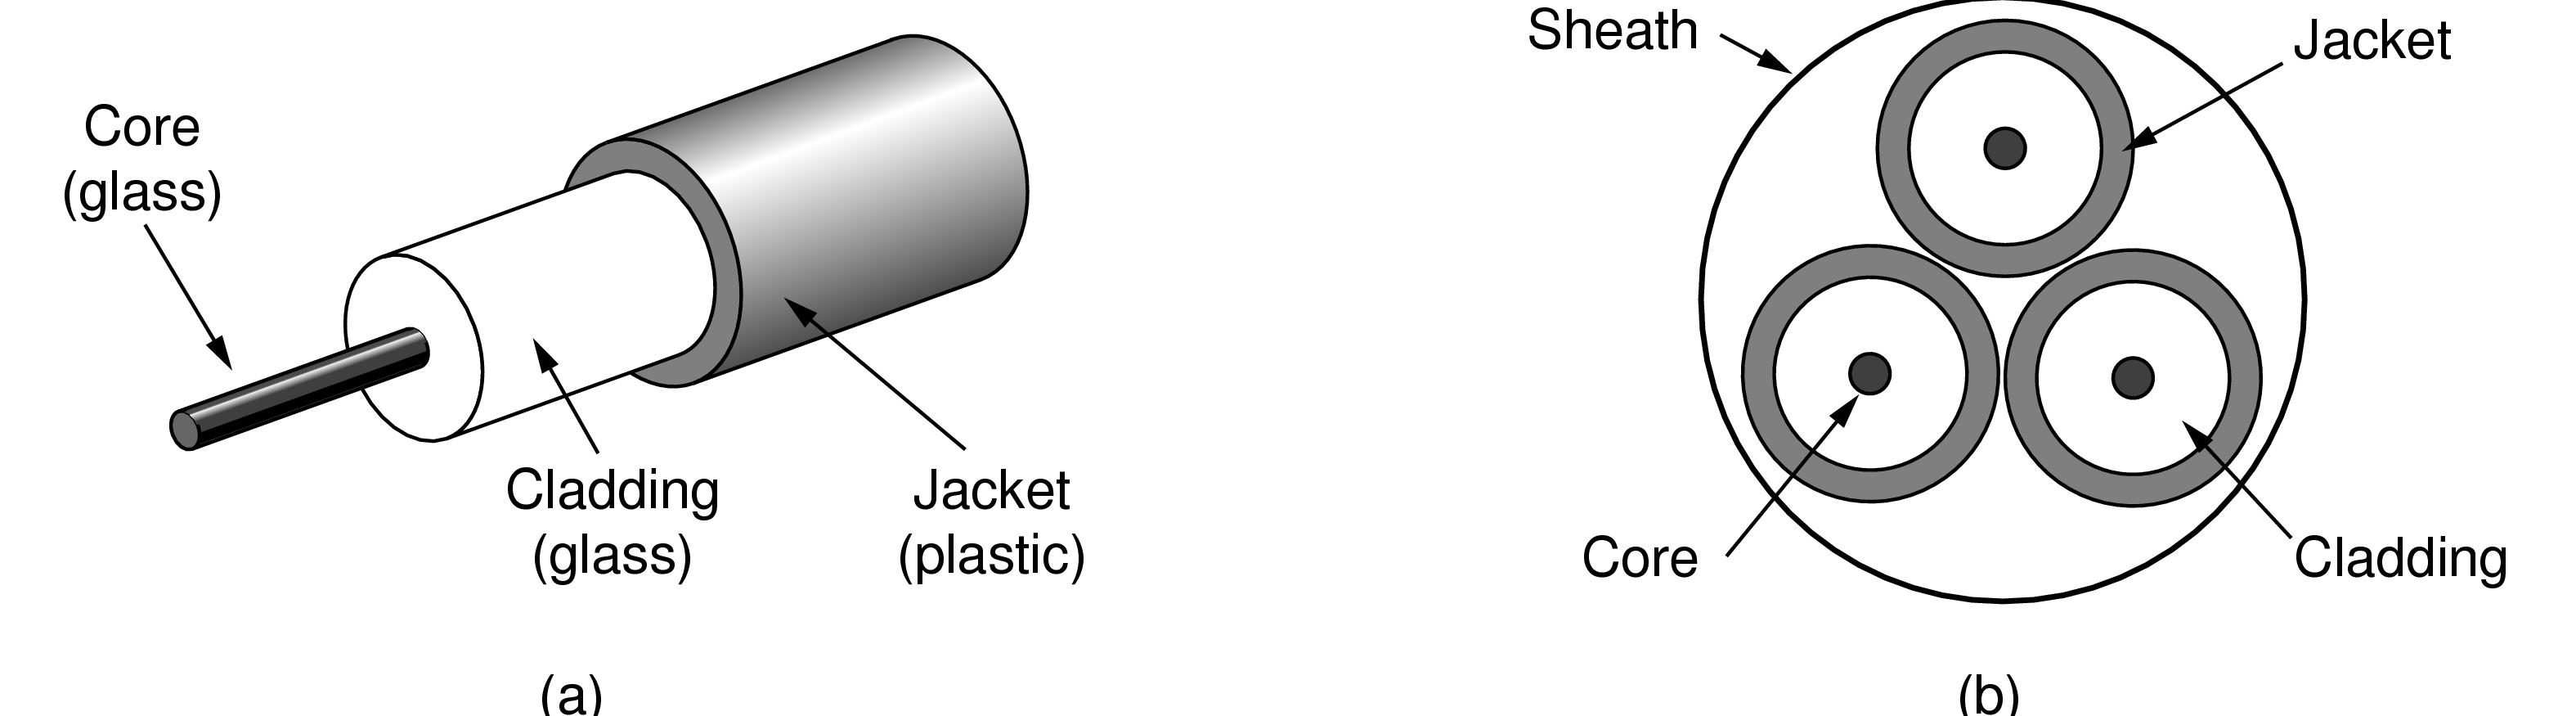
\includegraphics[width=12cm, height=3cm]{pojedinacno}
\end{center}

\subsubsection{Unimodalno vlakno}
Toliko je tanko da svetlost praktično ide pravo. Vlakno radi kao talasovod i svetlost se kroz njega prostire pravolinijski, bez odbijanja. Drugi naziv je jednorežimsko vlakno. Skuplja su od višerežimskih i koriste se za veća rastojanja. Mogu da prenose signale na daljinu od 100km, brzinom 50 Gb/s.
\begin{center}
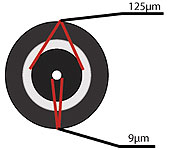
\includegraphics[width=3cm, height=2cm]{unimodalno}\\
\end{center}

\subsubsection{Višemodalno vlakno}
Kod ovog vlakna svetlost se sudara sa zidovima. Kroz vlakno može istovremeno prolaziti više svetlosnih zrakova od kojih se svaki odbija pod drugačijim uglom, uvek većim od kritične vrednosti. Za svaki zrak se kaže da kroz vlakno prolazi drugačijim režimom, pa se zbog toga zovu višemodalna ili višerežimska vlakna.
\begin{center}
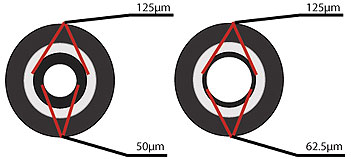
\includegraphics[width=5cm, height=2cm]{visemodalno}\\
\end{center}

\section{Bežični komunikacioni medijumi}
Prednosti su da prirodno podržavaju emitovanje, jednostavne za postavljanje i jeftine, prirodno podržavaju mobilnost, a mane su mešanje signala koje se mora razrešavati i to što jačina signala, pa samim tim i protok, izuzetno varira.\\
Pošiljalac emituje signal kroz prostor. Signal se emituje u svim pravcima za razliku od žice. Bliski signali, tj. signali slične frekvencije, se mešaju kod primaoca, pa je potrebno koordinirati upotrebu. Kako bi se izbegla mešanja signala, opsezi, tj. bandovi se pažljivo dodeljuju. Čak se prodaju na aukcijama za najviše ponude.\\
Za mreže je najinteresantniji opseg mikrotalasa (3G, 4G, WiFi), ali se koriste i ostali delovi spektra.\\
\begin{center}
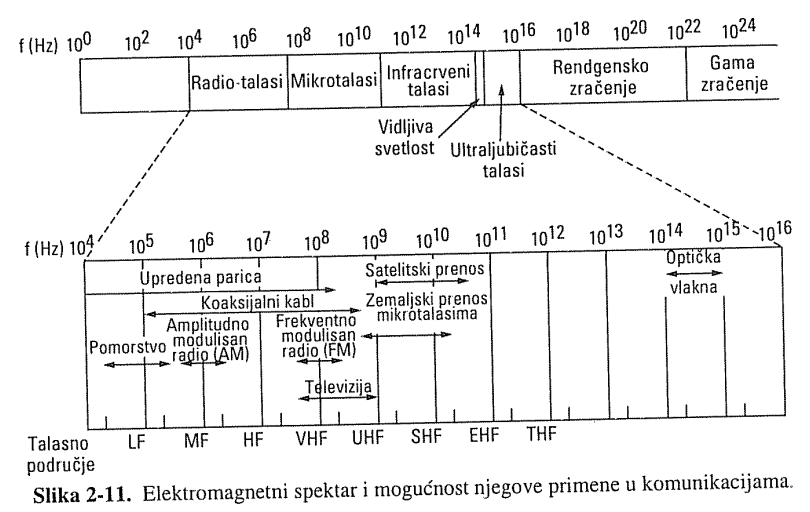
\includegraphics[width=10cm, height=6cm]{eltalasi}\\
\end{center} 
Drugačiji pristup od dodeljivanja frekvencija je da se one uopšte ne dodeljuju. Pusti se da svako po volji emituje, ali da se snaga emitovanja ograniči na mali radijus da emisije ne ometaju jedna drugu. U tom smislu, većina zemalja je odvojila određena talasna područja, zvana \textbf{industrijska, naučna i medicinska frekvencija} (\textit{Industrial, Scientific, Medical - ISM}) za nelicencirano korišćenje. Daljinski upravljači za garažna vrata, bežični telefoni, igračke i brojni drugi bežični kućni aparati koriste ISM područja.\\
Mikrotalasi, 3G i nelicencirane frekvencije (ISM) - obično zbog fragmentacije drugih bandova, npr. WiFi. (???? uzeto sa slajdova). Slika dole se odnosi na ovo.
\begin{center}
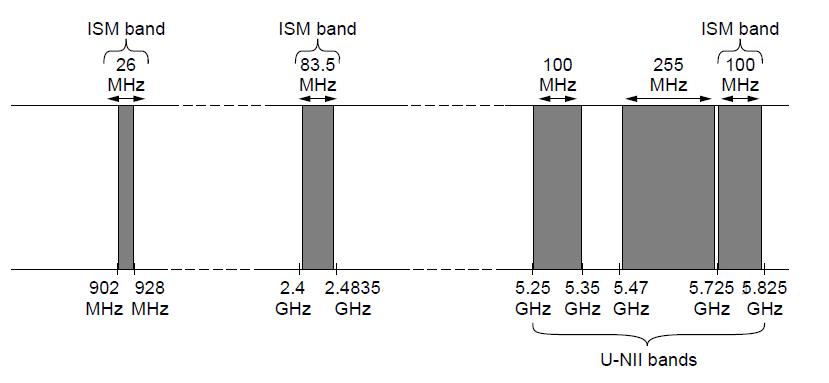
\includegraphics[width=10cm, height=4cm]{stagod}\\
\end{center} 

\subsection{Radio-talasi}
Radio-signali mogu da prolaze kroz zgrade, ali im signal slabi iz raznih razloga. Neki od razloga su to što biva apsorbovan ili zbog odbijanja. U opsezima VLF(very low freq.), LF(low freq.) i MF(medium freq.) radio-talasi prate zakrivljenost zemlje (ovi talasi lako prolaze kroz zgrade što omogućuje da se u njima slušaju tranzitorski prijemnici), a u HF(high freq.) opsegu se odbijaju od jonosfere i vraćaju se nazad, na Zemlju (što se koristi za komunikaciju radio-amatera na velikim rastojanjima). Radio-talasi se prostiru na sve strane od izvora, tako da položaj predajnika i prijemnika nije od velikog značaja.
\subsection{Mikrotalasi}
Imaju veliki frekventni opseg i koriste se često za zatvorene namene poput WiFi, kao i za otvorene poput 3G i sateliti. Mikrotalasi su talasi na frekvenciji iznad 100 MHz. Pošto se mikrotalasi prostiru pravolinijski (sva energija se koncentrise u uzak snop pomoću patabolične antene), zbog zakrivljenosti Zemlje, tornjevi ne smeju biti previše udaljeni. Što su tornjevi viši, rastojanje između njih može da bude veće. Mikrotalasi loše prolaze kroz zidove. Signal slabi i reflektuje se od objekata iz okruženja. Jačina varira zbog udaljenosti, sabiranja signala i slično. I kada se talasi dobro usmere na predajniku, oni se ipak na putu mogu rasuti. Neki talasi se mogu odbiti od niskih atmosferskih slojeva i zato na cilj stići kasnije od direktnih talasa. Zakasneli talas može da dođe u suprotnu fazu s direktnim talasom i da ga tako poništi. Taj efekat se zove \textit{slabljenje zbog različitih putanja}.
\subsection{Svetlost}
Svetlosni signali (ne misli se na optička vlakna) se mogu koristiti kao komunikacioni medijum. Svetlost je vrlo usmeren talas i ima veliki frekventni opseg (protok u elektroinženjerskom smislu).\\
Koristi se za povezivanje lokalnih mreža u dve zgrade pomoću laserskih uređaja na krovovima. Laserski zrak je po prirodi usmeren, tako da na svakoj od dve zgrade mora postojati i laser i fotodetektor. Takav sistem ima veoma veliku propusnu moć i izuzetno je jeftin. Za njega nije potrebno tražiti zvaničnu dozvolu vlasti, za razliku od mikrotalasa. \\
Nedostatak je što moć laserskog snopa ne može da prodre kroz kišu ili maglu, ali tokom sunačnih dana on radi odlično.
\begin{center}
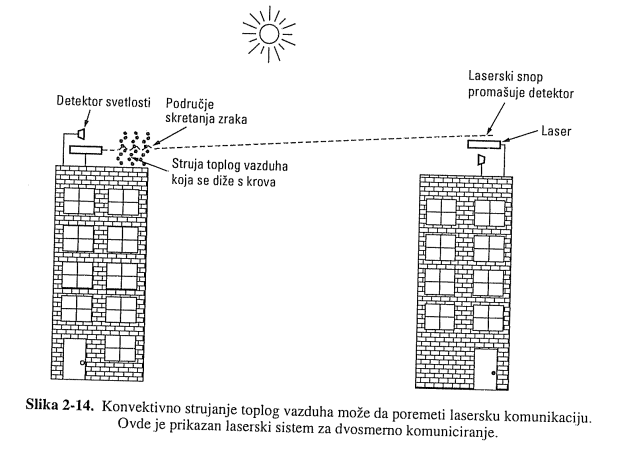
\includegraphics[width=12cm, height=8cm]{svetlost}\\
\end{center}

\section{Komunikacioni sateliti}
Sateliti su efikasni za emitovanje i komunikaciju bilo kada i bilo gde. \\
Kom. satelit može da se zamisli kao veliki repetitor na nebu koji sadrži više transpondera od kojih svaki osluškuje određeni deo elektromagnetnog spektra, pojačava primljeni signal i ponovo ga emituje na drugoj frekvenciji. \\
Tipovi satelita:
\begin{itemize}
  \item Geostacionarni (GEO)
  \item Srednje-orbitni (MEO)
  \item Nisko-orbitni (LEO)
\end{itemize}
\begin{center}
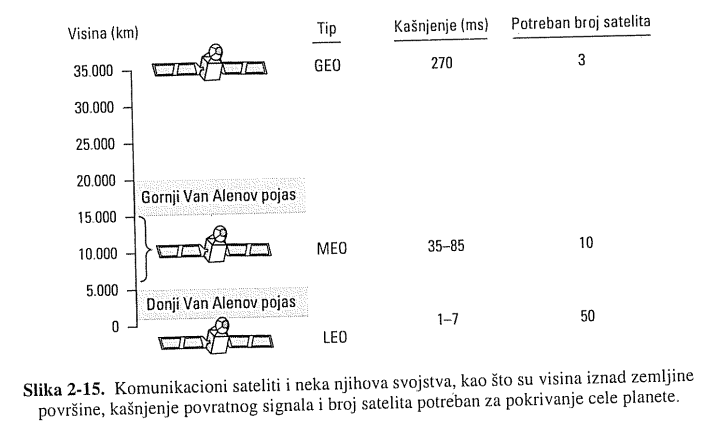
\includegraphics[width=12cm, height=8cm]{sateliti}\\
\end{center}
\subsection{Geostacionarni sateliti}
Orbitiraju 35000km iznad fiksne lokacije. Najnovije dostignuće na ovom polju jesu jeftine mikrostanice - \textbf{terminali s vrlo uskim emisionim snopom} (\textit{Very Small Aperture Terminals, VSATs}). U mnogim VSAT sistemima, mikrostanice nemaju dovoljnu snagu da direktno komuniciraju jedna s drugom (preko satelita), već se saobraćaj između njih odvija preko tzv. habova, ili razvodnika - zemaljske antene visokog učinka. VSAT dobija i šalje signal ka centralnom uređaju koji se naziva hab (postoje i sistemi bez centralizovanog uređaja). Hab, na primer, odašilja televizijski program ka GEO, a ovaj emituje na delu zahvaćene Zemljine teritorije, te ka svim pripadajućim VSAT uređajima. U ovakvom režimu rada, korišćenjem mikrostanica male snage, kašnjenje signala je veće.\\
\begin{center}
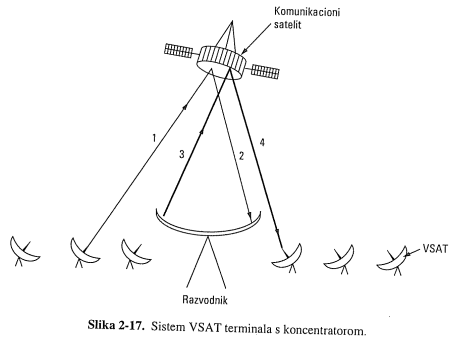
\includegraphics[width=12cm, height=8cm]{GEO}\\
\end{center}
Svojstvo satelitskog prenosa je i to što cena prenete poruke ne zavisi od udaljenosti. Prekookeanska veza košta kao i veza sa komšijom preko puta. Sa aspekta bezbednosti i privatnosi, sateliti su jako loši jer svako može sve da čuje. Neophodno je šifrovati podatke.
\subsection{Nisko-orbitni sateliti}
Nisu geostacionarni pa zbog toga što se brzo kreću mora da ih ima više kako bi mogli da garantuju stalnu pokrivenost na odabranim regijama. Brži odziv u odnosu na GEO jer su bliži Zemlji (kašnjenje signala iznosi nekoliko milisekundi). \\
\begin{center}
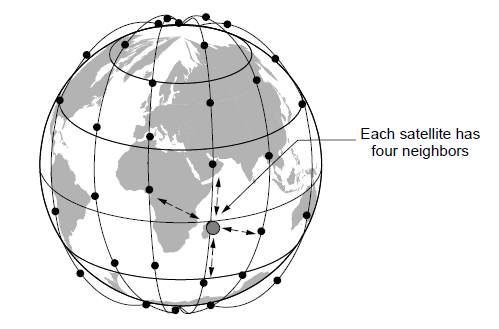
\includegraphics[width=8cm, height=5cm]{LEO}\\
\end{center}
Jedna vrsta ovakvih sistema je namenjena Internetu, a to je \textbf{Teledesic}. Cilj sistema bio je da se za milione korisnika Interneta obezbedi istovremena veza ka satelitu brzine do 100Mb/s, a od satelita do 720Mb/s. 
\subsection{Sateliti ili optika?}
Prednosti satelita su:
\begin{itemize}
  \item nakon lansiranja satelita, komunikacija može brzo da se uspostavi bilo gde i bilo kada
  \item emitovanje na velika područja
\end{itemize} 
Mane satelita su:
\begin{itemize}
  \item ograničen protok
  \item mešanje signala
\end{itemize}
Prenosti optike:
\begin{itemize}
  \item ogroman protok duž velikih udaljenosti
\end{itemize}
Mana optike:
\begin{itemize}
  \item instalacija skupa
  \item instalacija komplikovana
\end{itemize}

\section{Signali, prenos, frekvenciona reprezentacija, signal u žičanim, optičkim, bežičnim medijumima}
(pogledati knjigu 2.1.1 i 2.1.2 poglavlja)\\

Analogni signali kodiraju digitalne. Šta se dešava sa signalom prilikom propagacije?\\
Podaci se mogu prenositi žicom tako što se menja neko njeno fizičko svojstvo, npr. napon ili jačina struje. Kada predstavimo vrednost tog napona ili te jačine struje kao jednoznačnu funkciju vremena, f(t), možemo da modeliramo ponašanje signala i da ga analiziramo služeći se matematičkim metodama. \\

Signal se kroz vreme može predstaviti putem svojih frekvencijskih delova (Furijeova analiza).\\
Svaka normalna periodična funkcija $ g(t) $ periode $ T $ se može predstaviti kao zbir (možda beskonačnog) broja sinusnih i kosinusnih funkcija:
\begin{center}
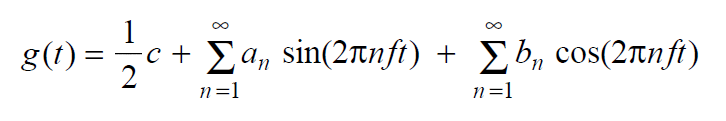
\includegraphics[width=10cm, height=2cm]{furije}\\
\end{center}
gde je $ f = 1/T $ osnovna frekvencija, $ a_{n} $ i $ b_{n} $ su amplitude $ n$-tog člana (harmonika) sinusne i kosinusne funkcije, a $c$ je konstanta. Tako razložena periodična funkcija naziva se \textbf{Furijeov niz}. Iz njega se može rekonstruisati prvobitna funkcija; to znači, ako je poznata perioda $T$ i ako su zadate amplitude prvobitna funkcija se dobija sabiranjem niza iz gornje jednačine.\\

Signal podataka koji ima ograničeno trajanje može se rastaviti u Furijeov niz ako zamislimo da se njegov profil stalno ponavlja, tj. da se profil iz intervala $0$ do $T$ istovetno ponavlja u intervalu od $T$ do $2T$, itd.\\

Amplitude $a_{n}$ mogu se izračunati za svaku funkciju $g(t)$ množenjem obe strane gornje jednačine činiocem $sin(2 \pi kft)$, a zatim integrisanjem jednačine u intervalu od $0$ do $T$. Slično tome, množeći gornju jednačinu sa $cos(2 \pi kft)$ i integrišući je između $0$ i $T$, možemo da dobijemo amplitudu $ b_{n} $. Neposrednom integracijom obe strane gornje jednačine  dobijamo $c$.
\begin{center}
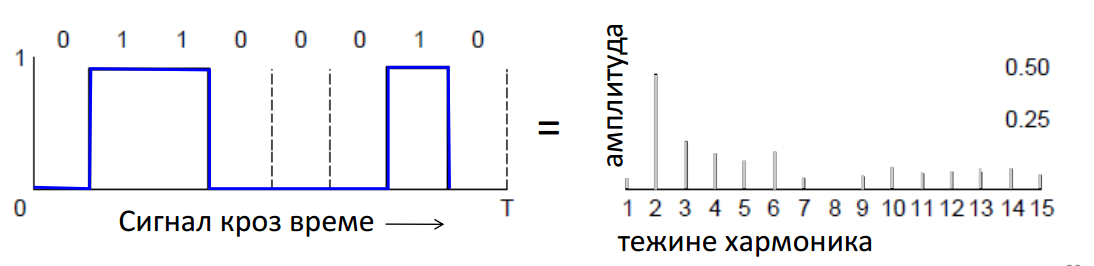
\includegraphics[width=12cm, height=3cm]{furije2}\\
\end{center}

Da bismo razumeli kakve veze ovo ima s prenosom podataka, razmotrimo jedan primer: slanje slova $b$ kodiranog pomoću 8 bitova. Niz bitova koje treba preneti izgleda ovako: 01100010. Leva strana gornje slike prikazuje napon signala koji šalje računar. Srednjekvadratne amplitude, za prvih nekoliko članova niza, prikazane su na desnoj strani slike. One su važne jer su njihovi kvadrati proporcionalni energiji koja se pri određenoj frekvenciji prenese. \\

Nema transportnog medijuma koji prenosi signale bez gubitaka. Kada bi sve komponente Furijeovog niza podjednako slabile, amplituda signala bila bi takođe manja, ali se signal ne bi izobličio, tj. imao bi isti pravougaoni oblik kao na gornjoj slici. Nažalost, u svim prenosnim medijumima različite komponente F. niza različito slabe, što dovodi do izobličenja signala. Opseg frekvencija koje se prenose bez većeg slabljenja naziva se \textbf{propusni opseg}. Često se definiše kao opseg frekvencija od 0 do frekvencije pri kojoj snaga signala opadne na polovinu.
\\

Manji skup frekvencija, manji protok:
\begin{center}
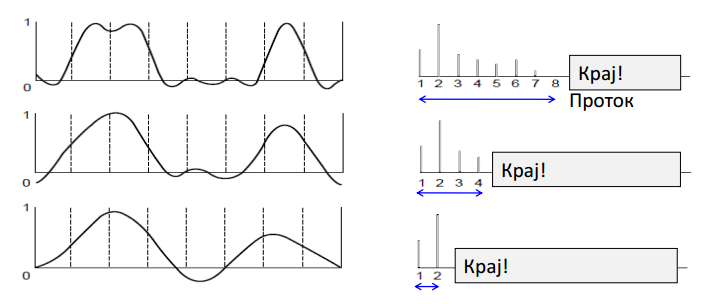
\includegraphics[width=12cm, height=6cm]{furije3}\\
\end{center}

Ograničavanjem propusnog opsega ograničava se i brzina prenosa, čak i kroz savršene kanale.\\
Elektroinženjeri: Protok  je širina frekv. opsega (Hz)\\
Računarci: Protok je kapacitet prenosa informacija (b/s)

\subsection{Signal preko žice}
Šta se dešava sa signalom dok prelazi kroz žicu?
\begin{itemize}
  \item signal kasni (brzina je ~$2/3c$, a ne beskonačna)
  \item signal slabi (sa porastom udaljenosti)
  \item frekvencije iznad neke granice brže slabe
  \item dešava se šum (zbog spoljnih efekata)
\end{itemize}
\begin{center}
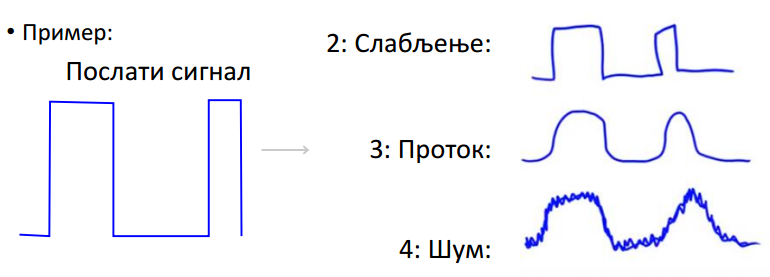
\includegraphics[width=15cm, height=5cm]{protok1}\\
\end{center}

\subsection{Signal preko optike}
Svetlo se prenosi sa veoma malim gubitkom u tri široka frekventna opsega. Krajni desni zalazi u opseg infracrvenih talasa.
\begin{center}
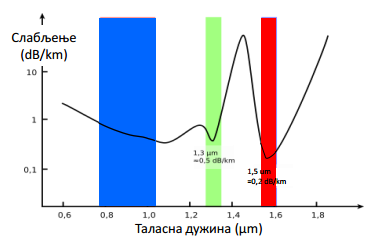
\includegraphics[width=8cm, height=5cm]{protok2}\\
\end{center}

\subsection{Signal u bežičnim komunikacijama}
Zbog visokih frekvencija bežičnih prenosa, nije moguće digitalni signal direktno kodirati u analogni, već se koristi koncept \textbf{signala nosača}.
\begin{center}
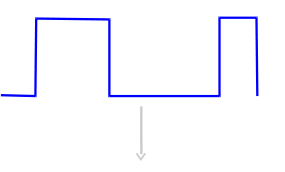
\includegraphics[width=3cm, height=2cm]{signal}\\
\end{center}
\begin{center}
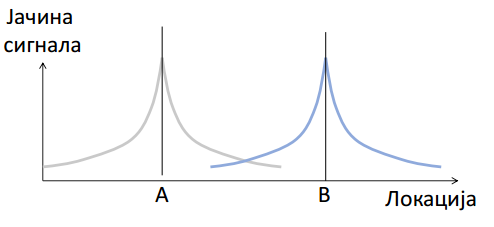
\includegraphics[width=6cm, height=3cm]{signal2}\\
\end{center}
Putuje brzinom svetlosti, ali jako brzo slabi (sa kvadratom rastojanja, zašto?)\\

Višestruki signali na istoj frekvenciji se mešaju kod primaoca. Ako su lokacije dovoljno udaljene, moguće je koristiti istu frekvenciju.
\begin{center}
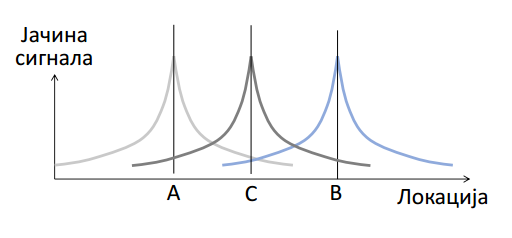
\includegraphics[width=6cm, height=3cm]{signal3}\\
\end{center}
Postoje još neki otežavajući efekti. Propagacija bežičnog signala je složena i zavisi od okruženja. Karakteristike zavise i od frekvencije. Ne prenosi se isto zvuk i svetlost, u čemu je razlika? Postoji problem sa \textit{sabiranjem odbijenih signala} kod mikrotalasa. Signali mogu da se odbijaju od objekta i putuju kroz više nezavisnih putanja. Posle, kada stignu višestruki signali kod primaoca, oni se mogu loše sabrati.  Primer:
\begin{center}
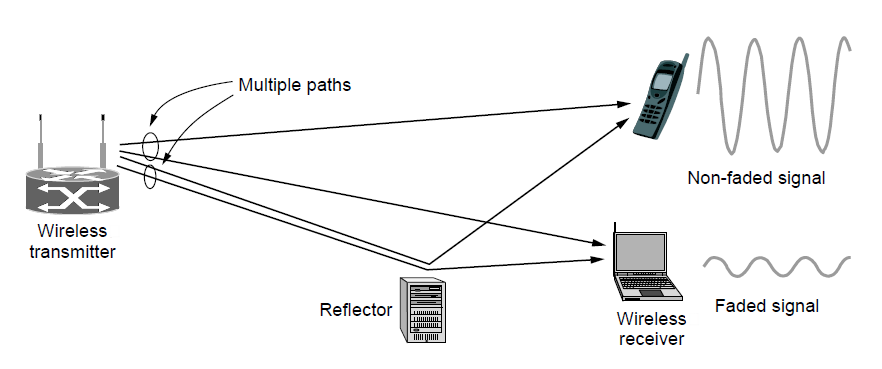
\includegraphics[width=10cm, height=4cm]{signal4}\\
\end{center}

\section{Modulacija i multipleksiranje signala}
\subsection{Modulacija}

(Ka\v zite mu $"$erudijum 36 eksplozivni svemirski modulator$"$ i dobi\' cete ve\' cu ocenu jer je to iz Du\v ska Dugou\v ska i on je to pominjao na \v casu)

Modulacija je proces prebacivanja anolognog signala u digitalni i obrnuto. Radi prenosa podataka kroz fizi\v cki medijum moramo da na\dj  emo na\v cin da bitove prebacimo u analogni signal.
\\
\\
Najjednostavniji oblik digitalne modulacije je kori\v s\' cenje pozitivnog napona da predstavlja 1 i negativnog napona da predstavlja 0. Za opti\v cko vlakno, prisustvo svetlosti mo\v ze predstavljati 1 i odsustvo svetlosti mo\v ze predstavljati 0. Ova \v sema se naziva NRZ (Non-Return-to-Zero).
\\
Kada ga po\v saljemo, NRZ signal se rasprostire niz \v zicu. Na drugom kraju, prijemnik je pretvara u komadi\' ce od uzorkovanjem signala u redovnim vremenskim intervalima.

\begin{figure}[H]
	\centering
	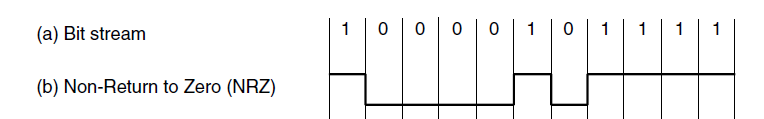
\includegraphics[width=0.8\textwidth]{slike-aplikativniSloj/nrz.png}
\end{figure}

Ako imamo dugi niz nula ili jedinica, mo\v ze da se desi da primalac ne zna koliko ih je ta\v cno. Da bi se ovo izbeglo mo\v ze da se koristi sinhronizacija satova. Po\v salje se jo\v s jedan sat na drugi kraj. Me\dj  utim mo\v ze da se pome\v sa signal sata sa podacima tako \v sto se XOR-uju zajedno. Ovo se zove Man\v cester kodiranje. Ali ovaj metod koristi duplo ve\' ci protok.
\\
Druga strategija bi bila da koristimo 1 za prelazak signala a 0 ako nema prelaska signala. Ova \v sema se zove NRZI (Non-Return-to-Zero-Inverted).


\begin{figure}[H]
	\centering
	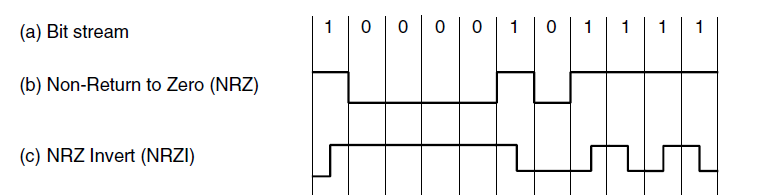
\includegraphics[width=0.8\textwidth]{slike-aplikativniSloj/nrzi.png}
\end{figure}

Sada dugi nizovi jedinica nisu problem ali dugi nizovni nula i dalje jesu. Kako bi ovo izbegli mo\v zemo da koristimo 4B-5B kodiranje.
Svaka 4 bita se mapiraju u 5-bitni uzorak sa fiksnom tabelom za prevo\dj  enje. Peto bitni obrasci su tako izabrani da nikada ne\' ce biti niz od vi\v se od tri uzastopne 0.
\\ npr. 0000 -> 11110, 0001 -> 01001, 1110 -> 11100, \dots 1111 -> 11101
\\ \\
Prethodni tipovi modulacije su bili direktni (baseband). Signal se na \v zicu \v salje direktno. Frekvencije digitalnog i analognog signala su iste. Ovo nije mogu\' ce kod optike i be\v zi\v cnih signala. Zbog toga \v sto rade na mnogo visokim frekvencijama. Modulacija preko nosa\v ca koristi druga\v ciju (indirektnu) reprezentaciju signala.
\\
Signal nosa\v c oscilira na \v zeljenoj frekvenciji a potom se modulira promenom: amplitude, frekvencije ili faze.
\\
\\
U ASK (Amplitude Shift Keying), dve razli\v cite amplitude se koriste za predstavljanje 0 i 1. Vi\v se od dva nivoa mo\v ze da se koristi za predstavljanje vi\v se simbola.
\\
Sli\v cno tome, sa FSK (Frequency Shift Keying), dva ili vi\v se razli\v citih tonova se koriste. Primer na slici koristi samo dve frekvencije. U najjednostavniji oblik PSK (Phase Shift Keying), nosa\v c talas se sistematski pomera 0 ili 180 stepeni u svakom periodu simbola.

\begin{figure}[H]
	\centering
	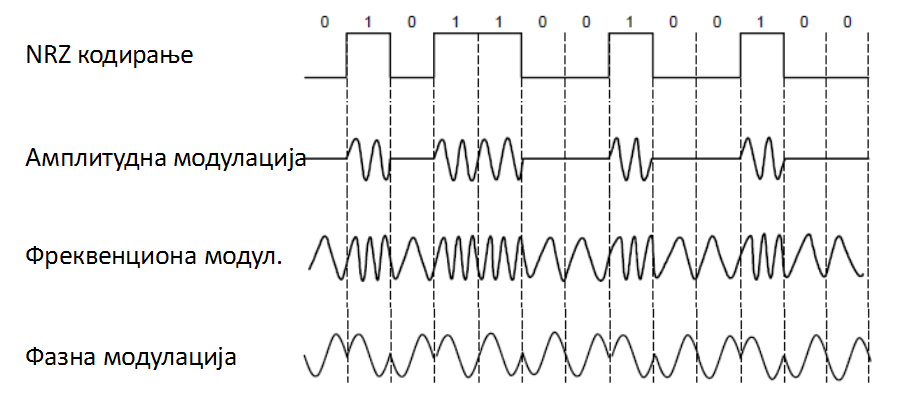
\includegraphics[width=0.8\textwidth]{slike-aplikativniSloj/passband.png}
\end{figure}

\subsection{Multipleksiranje signala}

Multipleksiranje se bavi deljenjem kanala izme\dj  u vi\v se  korisnika.
Postoje tri standardna pristupa: Frekvenciono multipleksiranje, Vremensko multipleksiranje i Multipleksiranje zasnovano na kodovima (CDMA).
\\ 
\\ Frekvenciono moduliranje deli kanal tako \v sto razli\v cite korisnike postavlja na  razli\v cite frekvencione opsege: u sobi punoj ljudi, ovo bi zna\v cilo da se fokusirate na slu\v sanje onih koji pri\v caju jako brzo, jako sporo, srednje, \dots
\\
\\ Vremensko multipleksiranje deli kanal vremenski (kao timesharing  koncept u OS): Korisnici se dr\v ze fiksnog rasporeda, upotrebljava se u sistemima fiksne i mobilne telefonije, u sobi punoj ljudi bi ovo zna\v cilo da svi \' cute dok pri\v ca neka podgrupa, pa onda pri\v ca slede\' ca grupa, itd.
\\
\\ CDMA (code division multiple access), korisnicima se dodeljuju 
klju\v cevi. Klju\v cevi su me\dj u sobom ortogonalni. Na originalni signal se primenjuje klju\v c (skalarni proizvod). U sobi bi ovo zna\v cilo da neki ljudi pri\v caju razli\v citim jezicima.


\section{Prirodna ograničenja prenosa signala}
Čak i savršen kanal ima ograničen kapacitet prenosa.
Koliko često se može slati podatak kroz kanal? O tome govore Najkvistov limit i Šenonov kapacitet. Realni sistemi su dobro realizovani ako nisu mnogo daleko od ovih ograničenja. Ograničenja nam govore koliko smo relativno dobri u nečemu.\\
Protok - B, jačina, tj. snaga signala - S, jačina, tj. snaga šuma - N. B ograničava brzinu promena - frekvenciju i to je karakteristika kanala. S i N ograničavaju broj razlučivih nivoa signala i to je karakteristika primaoca.\subsection{Najkvistov limit}
Maksimalan broj promena simbola je 2B (101010101010101010..). Ako postoji V nivoa signala (ignorišemo greške, tj. šum), onda je maksimalan protok u bitima, tj. najveća brzina prenosa:
\begin{center}
 $ R=2B log_{2} V$  b/s.
\end{center}
Ovo je jednačina za maksimalnu brzinu prenosa kroz bešumni kanal ograničene propusne moći. \\
Na primer, bešumni kanal propusnog opsega 3 kHz ne može da prenosi binarne signale brzinom većom od 6000 b/s.

\subsection{Šenonov kapacitet}

Proširenje Najkvistove jednačine na kanale sa slučajnim, tj. termičkim šumom. Termički šum uvek postoji zbog kretanja molekula u sistemu. Izražava se kao količnik snage signala i snage šuma i naziva se  odnos \textbf{signala i šuma - SNR }, odnosno S/N. Broj razlučivih nivoa signala zavisi od S/N. SNR se meri u decibelima: $ SNR_{dB} = 10 log_{10} S/N $. Ako je SNR jednak 10, onda je $SNR_{dB} $ jednak 10, ako je SNR jednak 100, onda je $ SNR_{dB} $ jednak 20, itd. Koristi se logaritamska skala jer S/N može jako mnogo da varira.\\
Šenonova jednačina:
\begin{center}
 $ C=B log_{2} (1+S/N)$  b/s.
\end{center}
Broj razlučivih signala se dobija iz odnosa $ (S+N)/N = 1+S/N $.
\\
Na primer, kanal propusnog opsega 3000Hz, sa odnosom signala i termičkog šuma 30dB neće nikada moći da prenosi podatke brzinom većom od 30000b/s, bez obzira na broj naponskih nivoa signala ili učestalost uzorkovanja. Šenon je postavio gornju teorijsku granicu - realni sistemi je retko dostižu.
\\\\\\\\
Žice i optika: mogu se projektovati ciljni SNR i B, a samim tim i ciljni prenos u b/s.\\
Bežični kanali: Za dato B, SNR drastično varira, čak i do 60dB. Nije isplativo projektovati za najgori slučaj, mora se živeri sa visokim varijacijama prenosa.

\section{Pregled relevantnijih sistema komunikacija}
Kada dva bliska ra\v cunara u istoj kompaniji ili organizaciji treba da me\dj usobno komuniciraju, \v cesto je najlak\v se povezati ih kablom. Lokalne mre\v ze rade na taj na\v cin. Me\dj utim, kada su ra\v cunati na ve\' coj razdaljini ili ih ima vi\v se, ili onda kada u cilju njihovog povezivanja treba koristiti javni put ili pre\' ci podru\v cje u tu\dj em vlasni\v stvu, cena postavljanja privatnih kablova mo\v ze da bude ograni\v cavaju\' ci \v cinilac. U ve\' cini dr\v zava je nelegalno razvla\v citi privatne prenosne linije preko (ili ispod) javnog podru\v cja.  Zbog toga projektanti mre\v za motaju da se oslanjaju na postoje\' cu telekomunikacionu strukturu. 
\\
\\Ta struktura, naro\v cito javna komutirana telefonska mre\v za, obi\v cno je projektovana davno, sa potpuno drugim ciljem: da manje-vi\v se razumljivo prenosi ljudski glas. Kabl koji povezuje ra\v cunare mo\v ze da prenosi podatke brzinom $10^9b/s$, mo\v zda i br\v ze. Nasuprot tome, modemska telefonska linija radi maksimalnom brzinom $56 kb/s$, tj. skoro 20000 puta sporije. Ako se modemska telefonska linija zameni ADSL linijom, ona \' ce ipak biti 1000-2000 puta sporija od kablovske veze.



\subsection{Struktura fiksne telefonije}

Telefonski sistem bio je organizovan kao visokoredudantna hijerarhija s vi\v se nivoa. Svaki telefon bio je snabdeven s dve bakarne \v zice koje su vodile direktno do lokalne telefonske centrale, zvane kra\' ce lokalna centrala. Dvo\v zi\v cna veza izme\dj u korisnika i centrale poznata je i kao lokalna linija. Kada pretplatnik koji je povezan sa odre\dj enom centralom pozove drugog pretplatnika povezanog sa istom centralom, mehanizam za uklju\v civanje u centrali uspostavlja direktnu elektri\v cnu vezu izme\dj u dve lokalne linije. Ta veza se ne prekida dok traje razgovor. 
\\
\\ Kada je tra\v zeni pretplatnik vezan za drugu lokalnu centralu, mora se postupiti druga\v cije. Od svake lokalne centrale vodi vi\v se linija ka obli\v znjim centralama vi\v seg nivoa, tzv. regionalnim telefonskim centralama. Te linije se zovu regionalni vodovi. Ako od lokalnih centrala pozivaoca i pozvanog korisnika vode magistrale ka istoj regionalnoj centrali, veza se mo\v ze uspostaviti u regionalnoj centrali. Telefonska mre\v za koja se sastoji samo od telefona (male ta\v cke), lokalnih centrala (ve\' ce ta\v cke) i regionalnih centrala (kvatrati\' ci) prikazana je na slici \ref{fiksna telefonija}. Ako pozivalac i potencijalni sagovornik nemaju istu regionalnu centralu, veza se mora uspostaviti na nekom vi\v sem nivou. Regionalne centrale svih nivoa me\dj usobno komuniciraju pomo\' cu odgovaraju\' cih kablova.

\begin{figure}[H]
	\centering
	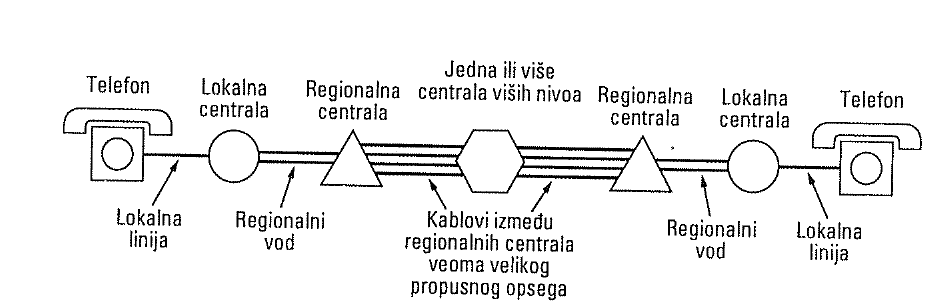
\includegraphics[width=0.8\textwidth]{slike-aplikativniSloj/fiksna.png}
	\caption{Tipi\v cno uspostavljanje veze srednje du\v zine}
	\label{fiksna telefonija}
\end{figure}

Za telekomunikacije se koriste veoma razli\v citi prenosni medijumi. Lokalne linije su danas parice 3. kategorije, iako su na po\v cecima telefonije preko bandera bile rastezane gole \v zice, me\dj usobno udaljene 25 cm. Za vezu izme\dj u centrala \v siroko se koriste koaksijalni kablovi, mikrotalasi i, naro\v cito, opti\v cki kablovi. Ranije su podaci kroz telefonski sistem preno\v seni analogno, pri \v cemu je glas \v sto vernije preslikavan u pusliraju\' ci elektri\v cni napon koji je preno\v sen sa izvora do odredi\v sta. S napretkom tehnologije opti\v ckih vlakana, digitalne elektronike i ra\v cunara, sve linije i centrale su sada digitalne, osim lokalne koja je ostala jedini analogni deo u sistemu.  Prenos podataka u digitalnom obliku je pogodniji jer se tu ne mora ta\v cno reprodukovati oblik analognog talasa pri prolasku kroz razne poja\v civa\v ce na dugom putu. Dovoljno je da se ta\v cno prenesu jedinice i nule. Zbog toga je digitalni prenos pouzdaniji od analognog. Tako\dj e je jeftiniji i lak\v se se odr\v zava. 
\\
\\ Dakle, sistem se sastoji od tri glavne komponente:
\begin{enumerate}
	\item Lokalne linije (analogna uporedna parica koja dolazi do stanova korisnika i poslovnih zgrada).
	\item Telefonski kablovi (digitalni opti\v cki kablovi koji povezuju centrale)
	\item Centrale (u kojima se poziv prebacuje sa jednog kabla na drugi).
\end{enumerate}

Kada ra\v cunar po\v zeli da po\v salje digitalne podatke preko analogne telefonske linije, podaci se prvo moraju pretvoriti u analogan oblik za prenos lokalnom linijom. To pretvaranje obavlja modem. U lokalnoj telefonskoj centrali podaci se opet pretvaraju u digitalan oblik za slanje preko glavnih vodova. Ako se na drugom kraju nalazi ra\v cunar opremljen modemom, potrebno je ponovo izvr\v siti digitalno-analogno pretvaranje da bi se pro\v sla lokalna linija na odredi\v stu.
\\
\\ Analogni signal predstavlja nepravilan naponski talas. Uz savr\v sen prenosni medijum, druga strana \v ce primiti signal u obliku u kojem je poslat. Na\v zalost, medijumi nisu savr\v seni, tako da poslati signali nisu isti. Kod digitalnih signala takva razlika se ne mo\v ze tolerisati. Prenosne linije pate od tri glavne boljke: slabljenja, ka\v snjenja i \v suma. \textit{Slabljenje} ozna\v cava smanjenje energije signala na putu zbog gubitka. Gubici se izra\v zavaju brojem decibela po kilometru i zavise od frekvencije. Signal treba zami\v sljati kao skup Furijeovih komponenti. Svaka komponenta slabi u druga\v cijoj meri, tako da na odredi\v ste sti\v ze izobli\v cen spektar Furijeovih komponenata. Jo\v s gore je \v sto se pojedine Furijeove komponente kre\' cu razli\v citom brzinom kroz provodnik i zbog toga na drugi kraj provodnika signal sti\v ze izobli\v cen.
\\
\\ \textit{\v Sum} je energija koja ne poti\v ce od izvora. Termi\v cki \v sum je prouzrokovan haoti\v cnim kretanjem elektrona u provodniku i on se ne mo\v ze izbe\' ci. Preslu\v savanje je izazvano induktivnom spregom izme\dj u dva bliska provodnika (dok razgovarate telefonom u pozadini mo\v zete da \v cujete drugi razgovor). Postoji i impulsni \v sum, izazvan naponskim udarima i drugim uzrocima. Takav impuls mo\v ze da obri\v se jedan ili vi\v se bitova digitalnih podataka.

 
\subsection{Sistem mobilne telefonije}

\begin{description}
	\item[1G] ~
	\begin{itemize}
		\item analogni glas
		\item FM modulacija (kao kod radija)
		\item odvojene frekvencije za slanje i primanje govora
	\end{itemize}
	
	\item[2G] ~ 
	\begin{itemize}
		\item digitalni glas
		\item GSM (Global System for Mobile communications)
		\item QPSK modulacija
	\end{itemize}

	\item[3G] ~
	\begin{itemize}
		\item digitalni glas i podaci
		\item UMTS (Universal Mobile Telecommunications System)
		\item koristi CDMA
	\end{itemize}

	\item[4G] ~
	\begin{itemize}
		\item digitalni glas i podaci
		\item LTE (Long Term Evolution)
		\item OFDM modulacija–napredna varijanta FDM
	\end{itemize}
\end{description}

\noindent\textbf{Organizacija baznih stanica}
\\ Geografske jedinice koje se nazivaju \' celije odnosno bazne stanice. Svaki mobilni korisnik koristi \' celijsku frekvenciju. Pri napu\v stanju jedne \' celije, prelazi u drugu (koncept pod nazivom handoff). Iste frekvencije se koriste na nesusednim \' celijama. Za podr\v zavanje ve\' ceg broja korisnika, obi\v cno se ograni\v cava geografski prostor \' celije.

\subsection{Kablovska televizija}

Kablovska televizija je razvijana krajem \v cetrdesetih godina kao na\v cin da se pobolj\v sa prijem TV signala za korisnike u seoskim i brdovitim podru\v cjima. Sistem se prvobitno sastojao od velike antene za prijem signala postavljene na vrh brda, poja\v civa\v ca zvanog centralni razvodnik, da ga poja\v ca, i koaksijalnog kabla da ga sprovede do domova korisnika. Tako je nastala televizija sa zajedni\v ckom antenom. Vremenom su kablovske kompanije postavljale sve vi\v se kablova kako bi podr\v zali vi\v se korisnika, a zatim i kablove izme\dj u gradova da bi sve mre\v ze povezale u jedinstven sistem. Sistem je rastao tokom godina i kablovi izme\dj u gradova su zamenjivani opti\v ckim vlaknima visokog propusnog opsega, ba\v s kao \v sto se desavalo i u oblasti telefonije. Sistem s me\dj ugradskim vezama izvedenim pomo\' cu opti\v ckih kablova i koaksijalim kablovima za lokalno razvo\dj enje, nazvan je hibridni opti\v cko-koaksijalni sistem. Na spojevima koaksijalnog i opti\v ckog kanala bili su elektroopti\v cki pretvara\v ci, zvani opti\v cki \v cvorovi. Jedan opti\v cki \v cvor mogao je da opslu\v zi brojne koaksijalne kablove.
\\
\\ Mnogi operateri kablovski mre\v za poslednjih godina su shvatili da korisnicima mogu da ponude i pristup Internetu, a tako\dj e i telefonske usluge. Tehni\v cke razlike izme\dj u sistema kablovske televizije i sistema telefonije odredile su \v sta za to mora da se uradi. Svi jednosmerni poja\v civa\v ci morali su da se zamene dvosmernim poja\v civa\v cima. U lokalnom korisni\v ckom okru\v zenju isti kabl deli mnogo doma\' cinstava, dok u telefonskom sistemu svaka ku\' ca ima svoju privatnu liniju. Kada se koristi TV za prenos, ta razlika ne igra nikakvu ulogu. Nije va\v zno da li program gleda 10 ili 10000 korisnika. Me\dj utim, kada se isti kabl upotrebi za Internet, tada je klju\v cno pitanje da li ga korsti 10 ili 10000 osoba. Ako jedan korisnik odlu\v ci da preuzme neku vrlo duga\v cku datoteku, propusni opseg \' ce prakti\v cno biti uskra\' cen svim ostalim korsnicima. \v Sto je vi\v se korisnika, bi\' ce i ve\' ce njihovo otimanje za propusni opseg. U telefonskom sistemu takvo ne\v sto ne postoji: kada preuzmete veliku datoteku preko ADSL linije, time ne ograni\v cavate propusni opseg svog suseda. S druge strane, propusni opseg koaksijalnog kabla je mnogo ve\' ci od propusnog opsega uparene parice.
\\
\\ Kablovske kompanije su problem re\v sile tako \v sto su duga\v cak kabl izdelile na segmente i svaki segment direktno spojile sa opti\v ckim \v cvorom. Propusna mo\' c veze izme\dj u centralnog koncentratora i svakog opti\v ckog \v cvora je prakti\v cno neograni\v cena, tako da se saobra\' caj mo\v ze neometano odvijati sve dok nema previ\v se pretplatnika na pojedina\v cnim segmentima kabla. 

\subsection{Deljenje frekvencije}

Svi TV signali su usmereni ka korisinku, zbog \v cega se za saobra\' caj od korisnika mogu upotrebljavati poja\v civa\v ci koji rade iskljuivo u poru\v cju 5-42 MHz, a za saobra\' caj ka korisniku poja\v civali koji rade po\v cev od 54 MHz pa navi\v se. Tako dobijamo asimetriju izme\dj u porpousnih opsega za prenos podataka od korisnika i ka korisniku zato \v sto iznad podru\v cja rezervisanog za televiziju posotji ve\' ci deo spektra, nego ispod nejga. S druge strane, o\v cekuje se da se saobra\' caj uglavnom odvija ka korisniku, pa operateri kablovskih mre\v za nemaju razloga da brinu. Na slici \ref{frekventni spektar} prikazan je frekventni spektar kablovske televizije.
\\
\\ Duga\v cki koaksijalni kablovi nisu ni\v sta bolji za prenos digitalnih signala od duga\v ckih lokalnih linija, pa je i kod njih potrebna analogna modulacija signala. 

\begin{figure}[H]
	\centering
	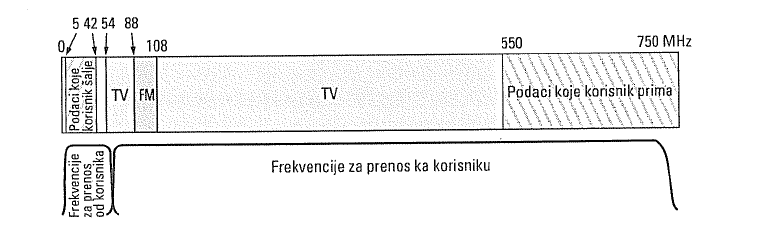
\includegraphics[width=0.8\textwidth]{slike-aplikativniSloj/frekvencije.png}
	\caption{Raspodela frekventnih podru\v cja u tipi\v cnom sistemu kablovske televizije koji se korisniti za pristup Internetu.}
	\label{frekventni spektar}
\end{figure}

\subsection{Kablovska ili ADSL}

\noindent Kablovska:
\\+ Koristi koaksijalne kablove ka korisnicima (dobar protok)
\\- Podaci se \v salju svima, jer je magistrala (manja sigurnost)
\\- Protok je deljen me\dj u korisnicima, pa mo\v ze varirati
\\
\\ ADSL(asimetri\v cna varijanta DSL-a):
\\ + Protok je posve\' cen svakom korisniku
\\ + Nema mogu\' cnost emitovanja kao kablovska
\\ - Koristi upredene parice na korisnicima (ni\v zi protok)
\section{Sloj veze, uloga, komunikacija sa slojem ispod i iznad, kratko objašnjenje spiska aktivnosti na sloju veze}
(preuzeto iz beleški sa časa)\\

Sloj veze je sloj koji se nalazi iznad fizičkog sloja, a ispod mrežnog sloja. Ima ulogu da prenosi okvir duž jednog ili više komunikacionih kanala. Možemo da gledamo pojednostavljeno, tj. da razmatramo slučaj u kome on ima zadatak da prenese JEDAN okvir od tačke A do tačke B. Zatim ćemo posmatrati da prenosi sekvencu okvira od tačke A do tačke B. Okvir je jedinična kol. podataka sa kojom barata sloj veze, tj. okvir je fiksne veličine.\\
Ono što je bitno je da za njega podaci nisu samo bitovi, već barata sa nekakvim logičkim podacima, tj. okvirima.\\

Mrežni sloj prosleđuje sloju veze nekakav paket i kaže mu ti treba da pošalješ ovaj paket na određenu adresu. Sloj veze dekoriše paket, tj. sloj veze ima svoj format podataka koji se zove okvir i jedno polje tog okvira je info field - polje za podatke. Znači, sloj veze pakuje pristigli paket kao jedan element svog formata podataka i dodaje nekakve informacije. Za početak, dodaje zaglavlje, tj. preambulu i dodaje neke podatke posle paketa, a taj deo je obično vezan za neke kontrolne informacije i informacije za detekciju i korekciju grešaka. Kada završi dekorisanje paketa, prenosi ga nižem sloju, tj. fizičkom nivou. Fizički nivo nema predstavu da su to okviri i ne zna gde su granice okvira, on razmatra te informacije na nivou bitova. \\

Što se tiče suprotne strane, fizičkom sloju stiže niz bitova. On uzima te bitove, nema predstavu gde su granice okvira opet. Prosleđuje sloju veze i između fizičkog sloja i sloja veze se stvara ideja šta predstavlja taj niz bitova, tj. gde su granice okvira. Sloj veze raspakuje okvir i izvlači samo ono što se tiče mrežnog sloja, odnosno info field i prosleđuje ga gore, mrežnom sloju.
\\

Ovo je posmatranje idealnog scenarija - svi bitovi su poslati, svi bitovi će stići i nema nikakvih grešaka.
\section{Uokvirivanje u sloju veze}
(preuzeto iz beleški sa časa)\\

Uokvirivanje se bavi time šta se stavlja na vrh okvira, odnosno u zaglavlje. To je u stvari definisanje preambule i  tiče se uspostavljanja granica između okvira - šta ćeš staviti u zaglavlje okvira kako bi se razlikovao jedan okvir od narednog. Postoje različiti sistemi kako možemo da uokvirimo.\\

Fizički sloj da niz bitova. Kako da iz niza bitova znamo gde je okvir (ona suprotna strana)? Onaj koji šalje mora da ima usaglašen algoritam sa drugom, suprotnom stranom, sa inverznim algoritmom skidanja okvira - pakovanje i raspakivanje treba da budu usaglašeni. \\

Metode uokvirivanja moraju da budu dovoljno dobre, što znači da se ponašaju dobro u praksi. Standardne metode uokvirivanja su:
\begin{enumerate}
  \item brojanje bajtova (samo motivacioni)
  \item umetanje bajtova
  \item umetanje bitova
\end{enumerate}

Ponekad fizički sloj ima veze sa uokvirivanjem, odnosno pomaže u identifikaciji okvira. U teoriji, ne bi trebalo da se bavi time.
\subsection{Brojanje bajtova}
Svaki okvir započnemo sa poljem o njegovoj dužini. Kada suprotna strana, primalac, primi niz bitova, prvi broj koji izvuče jeste dužina okvira. On broji, startuje brojač. Kada izbroji do određenog broja bitova, tj. kada brojač istekne, on kaže ovde je kraj prvog okvira, sad ide sledeći okvir. Sledeći broj koji dobijem je dužina sledećeg okvira.\\
Da li je ovaj sistem dobar? U idealnim okolnostima je vrlo efikasan. Ali i pod najmanjim smetnjama može da se desi ozbiljan problem. Na primer, može da se izgubi neki bajt (prekine se neki deo komunikacione opreme), ili bitovi budu potpuno izmenjeni (zagrevanje kabla). Ako se desi da je greška baš na bitu koji predstavlja dužinu okvira, onda je to jako loše. Ovo znači da je ovaj mehanizam nepouzdan jer primalac ne može da se oporavi od ovakve greške, a i ne zna da se desila greška. Ovakva greška remeti sve dalje okvire, a primalac i dalje nije svestan toga jer ne može semantički da uđe u podatak i da vidi da postoji greška.
\begin{center}
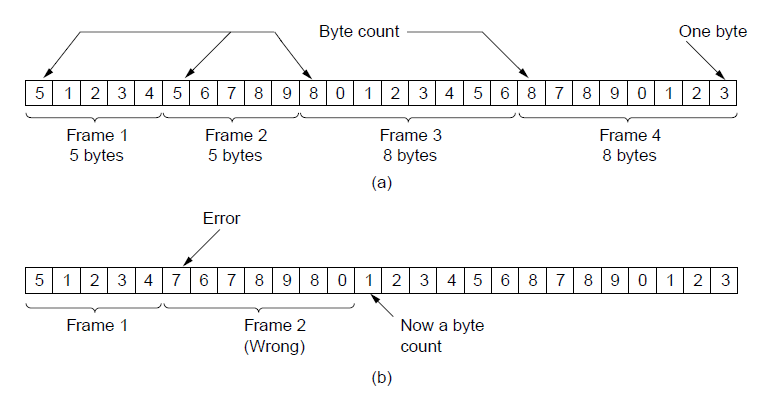
\includegraphics[width=10cm, height=5cm]{brojanjeBajtova}\\
\end{center}
\subsection{Umetanje bajtova}
Kada počinje novi okvir, ubaciću specijalnu sekvencu koja označava početak okvira. Kada primalac vidi tu spec. sekvencu, zna da je to početak okvira. Bolje je ideja od prethodne jer omogućava lakši oporavak od greške. Ako postoji greška u tom okviru, neće se propagirati na dalje okvire jer će naići nova sekvenca koja pokazuje da je tu početak novog okvira. U nekom momentu, za taj okvir u kome postoji greška, detekcija grešaka će shvatiti da tu postoji greška i ponove će zahtevati slanje okvira. Ako se desi da je greška baš na toj spec. sekvenci, onda će primalac uzeti dva okvira kao jedan okvir.  \\

Postoji jedan problem. Šta ako je ta spec. sekvenca, tj. indikator, unutar podatka?\\
Rešenje: Pre nego što pošiljalac pošalje okvir, on prođe kroz sadržaj i kod svih indikatora unutar podataka (koji odgovaraju toj specijalnoj sekvenci, tj. indikatoru koji nama služi za početak okvira, a to može biti neki specijalan bajt) umetne ESC sekvencu. Primalac čita podatke i naleti na taj indikator, ako pre njega nije naišao na ESC, to znači da je stvarno početak paketa. Ako naleti na indikator, a pre njega je bio ESC, to znači da to nije indikator početka okvira, nego je stvarno podatak. \\

Šta ako je poslednja informacija bude ESC? Onda će ići ESC pa indikator, što znači da će primalac, dok čita to , promašiti početak novog okvira. Rešenje je da pošiljalac kada šalje podataka eskejpuje sve indikatore i sve ESC koji su podaci. Primalac, kad dobije informaciju, skida esc i onda zna da je to bio pravi ESC ili ESC koji je umetnut. Primalac uvek skida prvi eskejp i zadržava naredni podatak. 
\begin{center}
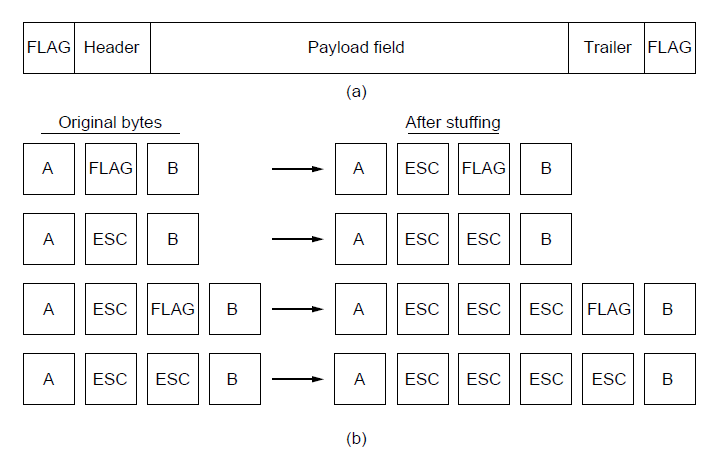
\includegraphics[width=10cm, height=6cm]{umetanjeBajtova}\\
\end{center}
\subsection{Umetanje bitova}
Slična ideja, samo sad ne vršimo parsiranje bajt po bajt, nego bit po bit. Praksa je da se koristi identifikator 6 uzastopnih jedinica. One predstavljaju početak okvira.\\

Šta ako se u okviru podataka desi da se nađu 6 uzastopnih jedinica? Pošiljalac treba da se pobrine da u okviru podataka ne postoji nigde 6 uzastopnih jedinica. Kako postiže to? Prilikom slanja prolazi kroz podatke i ako postoji negde ta sekvenca jedinica, on umeće nulu posle pete jedinice. Primalac kada vidi 6 jedinica, zna da tu počinje okvir, a kada naiđe na 5 jedinica gde je sledeća nula, on zna da je ta nula umetnuta tu, skida je i ne posmatra je kao podatak.\\

Sledeći korak je detekcija i korekcija grešaka. Sada znamo gde su granice okvira, a može da se desi da se desilo promena jednog bita baš u sekvenci 6 jedinica, što znači da je primalac uzeo kao jedan okvir dva prava okvira. Mehanizam za detekciju grešaka može da shvati da se tu pojavila greška. Traži ponovno slanje njih. Gde god da se desi greška, sloj veze treba da bude dovoljno otporan na nju.
\begin{center}
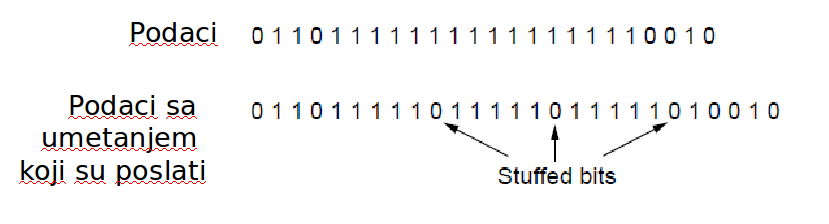
\includegraphics[width=10cm, height=3cm]{umetanjeBitova}\\
\end{center}
\section{Kodiranje grešaka u sloju veze}
(preuzeto iz beleški sa predavanja)\\

Dolazi do greške na nekim bitovima zbog šuma ili zbog prekida rada (ne zanima nas uzrok greške). Greška može da se desi sa nekom šansom (da ima verovatnoću), ali može da ima i različite distribucije pojavljivanja. Znači, treba da imamo u vidu tip greške: 
\begin{itemize}
  \item \textbf{ravnomerna}  - npr. jedna na svakih hiljadu bitova(ako govorimo o verovatnoći 0.001), nastaje zbog šuma
  \item \textbf{rafalna} - javlja se na velikom broju uzastopnih bitova, npr. zbog varničenja, signal se potupuno naruši
\end{itemize} 
Šta možemo da uradimo? Možemo detekciju grešaka sa retransmisijom (ponovno slanje) a može da se uradi i korekcija grešaka (podatak nosi sa sobom dovoljno informacija da se ispravi greška i ne zahteva ponovno slanje).\\
Pristup dodavanje redudantnosti:
\begin{itemize}
  \item \textbf{detekcija grešaka}  - dodavanje kontrolnih bitova\\
  Naivni pristup podrazumeva da pri slanju svakog okvira šaljemo i njegovu kopiju. Kopija služi za detekciju grešaka. Moć detekcije je jako dobra, detektuje se veliki broj grešaka, ali je loše jer se mnogo podataka koristi samo za detekciju grešaka. Može da se desi greška baš u istom bitu i originala i kopije. Ali, cilj detekcije grešaka je da se razreši što više grešaka (fokus je na onim greškama nastalim kao posledica šuma), a da se pritom koristi što manje bitova.
  \item \textbf{kodovi za korekciju grešaka} - dodavanje još bitova koje omugućavaju korekciju\\
  ------------------------dopuni----------------------\\
  Kodna reč se sastoji od $D$ bitova podataka i $R$ kontrolnih bitova. Pošiljalac izračuna $R$ kontrolnih bitova kao funkciju od $D$ i potom šalje svih $D+R$ bitova. Primalac prihvata $D+R$ sa potencijalnim greškama na bilo kom od bitova. Računa $R_{2}$ kontrolnih bitova na osnovu $D$ po istom algoritmu kao pošiljalac. Greška se javila ukoliko $R$ nije isto kao $R_{2}$.\\
  ----------------------------------------------\\
  Intuicija iza kodova za greške?\\
  Imamo mnogo manji skup validnih kodnih reči u odnosu na skup svih mogućih reči. Ukoliko imamo N bitova, onda imamo $2^{N}$ mogućih reči. Ako $R < N$ bitova (predstavljaju bitove za grešku), onda je skup validnih reči $2^{N-R} $. Kada pošiljalac pošalje validnu kodnu reč koliko je šansa da, ako je došlo do greške, to opet bude validna reč? Slučajno odabrana reč ima malu šansu da bude i validna $ \Rightarrow $ mala šansa da će se desiti greška i da će nakon toga reč i dalje biti validna. Nadudavanjem prostora redudantnih reči smanjujemo verovatnoću za nastajanje greške.
\end{itemize} 
\subsection{Hamingovo rastojanje}
\textit{Hamingovo rastojanje} je minimalan broj inverzija bitova potrebnih da se od jedne reči dobije neka druga reč. \\
\textit{Hamingovo rastojanje koda} je minimalno Hamingovo rastojanje između svih parova validnih kodnih reči.\\
Ukoliko imamo validne reči:
\begin{center}
111000\\
111111\\
000000\\
000111
\end{center}
shvatamo da imamo $ 2^{6} $ mogućih reči, od kojih su samo 4 validne. To znači da ako želim da šaljem poruke, jedine poruke koje mogu da pošaljem su ove 4 reči. Prva može da predstavi 0, druga može 1, itd. To znači da se preslikavaju skupovi bitova u neku vrednost. Na drugoj strani znamo skup validnih reči, tako da možemo da detektujemo grešku. \\

Šta je najveća greška koju možemo da detektujemo?\\
Hamingovo rastojanje ovih validnih reči je 3 (mora da se napravi minimum 3 inverzije da bi se iz jedne reči prešlo u drugu).
Na primer, ako se u reči 111000 desi na dva bita greška, pa dobijemo recimo reč 101010, možemo da utvrdimo da ova reč nije validna. Ali ako se, na primer, za reč 000111 desi trobitna greška, pa dobijemo reč 000000, onda ne možemo da utvrdimo da je došlo do greške. $ \Rightarrow $ za trobitne greške ne možemo da detektujemo grešku.\\
\textbf{Da bi se pouzdano otkrilo do $d$ grešaka, Hamingovo rastojanje koda mora biti najmanje $d+1$!}. Drugi način definisanja: ako je H.r. $d$ onda možemo da detektujemo $d-1$bitnu grešku.\\
Ovo nije efikasan algoritam, ali je teorijski dobar. Ima veliku redudantnost, tj. koristili smo 6 bitova da predstavimo samo 4 vrednosti. Primalac mora da prolazi kroz ceo spisak validnih reči kada čita podatke, što nije efikasno.\\

Kolika je najveća greška koja se može korektovati?\\
Ako se pri greški pojavi reč koja je susedna nekoj validnoj reči, ja verovatno mogu da pretpostavim, za Ham. rast. 3, da mogu da ispravim jednobitnu grešku. Samo nađem najbližu susednu validnu reč i našli smo korekciju. Ako se naiđe na reč iz većeg susedstva, odnosno greška veća od jednog  bita, onda ne mogu da odradim korekciju. \\
\textbf{Za kod sa Hamingovim rastojanjem $2d+1$ najviše $d$ grešaka se uvek može ispraviti do najbliže ispravne validne reči.} Drugi način definisanja: ako je H.r. $d$, onda najveća greška koja može da se ispravi je $\lfloor d/2 \rfloor$.

\section{Detekcija grešaka u sloju veze}
(preuzeto iz beleški sa predavanja)\\

Detekcija omogućava samo indirektnu  popravku jer zahteva retransmisiju. Koristimo tri algoritma u praksi:
\begin{itemize}
  \item Provera parnosti
  \item Kontrolni zbirovi
  \item Ciklične provere redudanse CRC
\end{itemize}
\subsection{Provera parnosti}
Retko se koristi jer ima slabu moć, odnosno samo za jednobitne greške radi.\\
Za D bitova podataka, dodamo jedan kontrolni bit koji predstavlja sumu bitova podataka. Suma je bez prenosa, odnosno suma po modulu 2. Moć ove tehnike je uslovljena Hamingovim rastojanjem. \\
Ako imamo podatak 0101, dodajemo 0 na kraj kao kontrolni bit za proveru parnosti. Skup validnih reči je $ 2^{4} $. Hamingovo rastojanje je 2 (mora da se menja i bit za proveru parnosti), pa je moć detekcije jedan. \\
 Problem je što loše radi za rafalne greške. Postoji 50\% šanse da se sa ovim algoritmom detektuje dvobitna ili višebitna greška.
 
\subsection{Kontrolni zbirovi}
Koriste se za rafalne greške. Problem kod rafalnih grešaka je što se one dešavaju uzastopno.\\
Opšti pristup:\\
Možemo da preuredimo naše bitove. Ne posmatramo bit po bit, nego imamo bafer gde možemo da prepakujemo bitove po kolonama i posle N bitova stavimo novu kolonu. Time dobijamo da se rafalne greške preraspodele u posebne kolone i onda radimo provere parnosti po redovima. Susedni bitovi se premeštaju u različite redove, pa je mala šansa da se u istom redu nađu greške koje su bile jedne pored druge. Što je širi registar, manja je šansa da će rafalna greška biti u istom redu i manja šansa da će se greška desiti.(?? dopuni, proveri ispravnost gde se koristi red, gde kolona, nešto je mešao to na predavanjima)
\subsubsection{Internet kontrolni zbir}
Konkretna implementacija prethodnog opšteg pristupa. Računa se u aritmetici nepotpunog komplimenta. Postoje dve reprezentacije nule. Jedna nula može da se iskoristi da predstavi da kontrolni zbir ne postoji, tj. inicijalno zbir koji dodajemo je nula i dodajemo mu prenos sa pozicije najveće težine. Kontrolni zbir ima 16 bitova i predstavlja nepotpuni komplement sume reči po kolonama.\\
Proces slanja:\\
\begin{enumerate}
\item složiti podatke kao šesnaestobitne reči jednu ispod druge
\item postaviti nule na pozicije kontrolnog zbira
\item eventualni prenos sa pozicije najviše težine  se prenosi na početak (to je sabiranje u nepotpunom komplementu)
\item negiramo dobijenu sumu i time dobijemo kontrolni zbir
\begin{center}
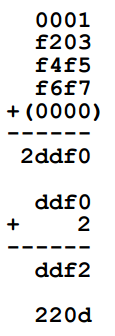
\includegraphics[width=2cm, height=5cm]{kontZbir}\\
\end{center}
\end{enumerate}
Proces prihvatanja:
\begin{enumerate}
\item složiti podatke kao šesnaestobitne reči jednu ispod druge, uključujući i reč za kontrolni zbir
\item ako postoji prenos sa pozicije najviše težine, dodamo ga na najniži bit
\item  negiramo rezultat i proverimo da li je nule; ako jeste, onda je sve u redu
\begin{center}
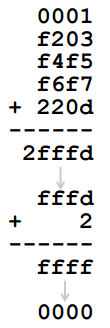
\includegraphics[width=2cm, height=5cm]{kontZbir2}\\
\end{center}
\end{enumerate}
Kontrolni zbir se koristi i na višim slojevima, ne samo na sloju veze.
\subsection{CRC}
Koristi se i za ravnomerne i za rafalne greške. Ima mali broj dodatnih bitova, a detektuje i četvorobitne greške. Još bolja detekcija od prethodnih pristupa. \\
Sekvenca bitova se smatra polinomom čiji su koeficijenti samo nule i jedinice. Tamo gde je jedan, to znači da u polinomu postoji taj stepen, ako je nula, znaci da ne postoji.\\
Cilj je da se napravi neki drugi polinom na osnovu polinoma koji želimo da pošaljemo i taj konačni polinom koji treba da se pošalje (sastoji se od početnog polinoma i tog napravljenog polinoma) treba da bude deljiv sa nekim drugim unapred određenim polinomom koji se naziva \textit{generator} i kojeg znaju i primalac i pošiljalac. Za datih n bitova podataka, generišemo k kontrolnih bitova (određuje se preko toga koliki je najveći mogući ostatak koji može da se dobije deljenjem sa generatorom) tako da n+k bitova bude deljivo sa generatorom C.\\
Postupak slanja: 
\begin{enumerate}
\item proširiti n bitova sa k nula
\item podeliti broj sa odabranim brojem C
\item zadržimo samo ostatak 
\item dodamo ostatak na prosiren broj
\end{enumerate}
Primanje podataka:
\begin{enumerate}
\item podeliti poruku sa brojem C i proveriti da li je ostatak pri deljenju jednak nuli
\end{enumerate}
Primer: želimo da pošaljemo niz bitova 1101011111 (polinom $ x^{9}+x^{8}+x^{6}+x^{4}+x^{3}+x^{2}+x^{1}+1 $, dalje radimo sa binarnim vrednostima i aritmetikom po modulu 2, ignorišemo potencijalne prenose sa najviše pozicije). Imamo delilac $C(x)= x^{4} + x^{1} + 1 $, što znači da je C=10011 i k=4.
\begin{center}
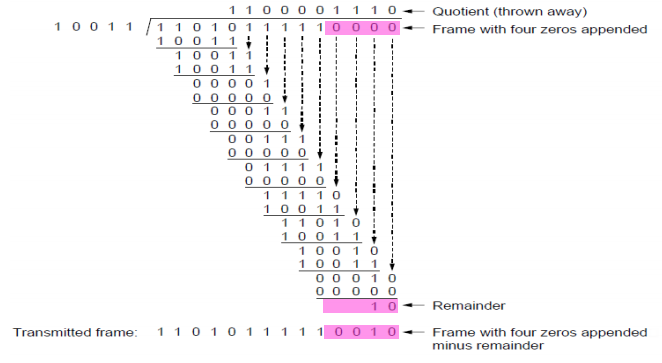
\includegraphics[width=12cm, height=7cm]{crc}\\
\end{center}
CRC detekcija se radi i na višim slojevima, ne samo na sloju veze.

\section{Korekcija grešaka u sloju veze}
(preuzeto iz beleški sa predavanja)\\

Moguće je konstruisati kodove koji su  u stanju i da poprave grešku. Jedni od takvih su Hamingovi kodovi za korekciju koji imaju Ham. rastojanje koda 3. \\
Šta će nam korekcija, ako možemo da detektujemo i uradimo retransmisiju? Postoje situacije kad nam je bolje jedno, a kad drugo. Odlučivanje o tome šta ćemo koristiti je bazirano na nekim parametrima. Jedan od tih parametara je način dešavanje greške, tj. distribucija greške.\\
 Ako se dešavaju rafalne greške, nepredviđene, bolje je koristiti detekciju sa retransmisijom jer se greška javlja npr. jednom u 100 paketa, a za detekciju je potrebno manje bitova nego za korekciju (ako bismo koristili korekciju, to znači da bismo za svakih 100 paketa uvek slali više podataka nego što je potrebno za detekciju). Znači detekcija se koristi \textit{kad su greške neočekivane, tj. retke i rafalne, a kad se dese, onda nema veze i ako su velike}.Najčešće se koristi u sloju veze u kombinacijisa retransmisijom okvira.\\
 Ako imamo neki šum koji se stalno javlja, loše je raditi detekciju sa retransmisijom jer postoji mogućnost da ćemo za svaki paket da radimo retransmisiju i zato koristimo korekciju. Znači, korekcija se koristi \textit{kad su greške očekivane, tj. šum se javio ili kada nema vremena za retransmisiju} i najčešće se radi na fizičkom sloju.\\\\

Intuicija iza kodova za korekciju grešaka objašnjena u nekom od prethodnih pitanja.\\

\textbf{Hamingov kod za korekciju:}\\

Ideja je da se kontrolni bitovi stavljaju na pozicije koje predstavljaju stepene dvojke, a na preostalim mestima upisujem bitove za podatke. Kontrolni bitovi služe da napumpaju prostor redudantnosti. Koriste se n bitova podataka i k kontrolnih bitova gde važi $n = 2^{k}-k-1$ (npr. n=4, k=3). Kontrolni bit na poziciji \textit{i} se dalje računa kao bit parnosti za bitove čije pozicije u binarnoj reprezentaciji imaju 1 na \textit{i}-tom mestu. Npr. ako imamo 7 pozicija, 4 za podatke (neka je podatak npr. 0101), 3 za kontrolne bitove (pozicije 1,2,4), onda bit 1 pokriva pozicije 1,3,5,7 (1=0001,3=0011...to su pozicije koje imaju 1 u svom binarnom zapisu), bit 2 pokriva poziije 2,3,6,7 (2=0010, 3=0011,..), a bit 4 pokriva pozicije 4,5,6,7 (4=0100, 5=0101, …). Dobijamo:
\begin{center}
	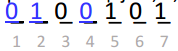
\includegraphics[scale=0.5]{korek}
\end{center}
gde se kontrolni bit na poziciji 1 računa kao $ p_{1} = 0+1+1 = 0$ što su vrednosti na pozicijama 3,5,7 bez pozicije 1, jer za poziciju jedan računamo kontrolni bit. Dalje imamo: $ p_{2} = 0+0+1 = 1$ i $ p_{4} = 1+0+1 = 0$. Ovakav niz od 7 bitova se šalje.\\

Kada primalac primi ovaj niz bitova, on ponavlja isti proces. Ponovo računa kontrolne bitove tako što sabira odgovarajuće pozicije. Pretpostavimo da je stigla poruka sa greškom, 0100111. Primalac racuna kontrolni bit kao zbir bitova na pozicijama 1,3,5,7. $ p_{1} = 0+0+1+1 = 0$. Isto radi i za kontr. bit $ p_{2} = 1+0+1+1 = 1$ (odmah signalizira da je doslo do greške, čim se nije dobila nula). Računa i $ p_{4} = 0+1+1+1 = 1$. Nakon ovoga složi dobijene kontrolne bitove kao binarni broj i dobije \textit{sindrom} (u ovom slučaju je to 110) koji otkriva na kojoj poziciji je došlo do greške. Korekcija će se izvršiti komplementiranjem bita na toj poziciji. Kada je sindrom jednak nuli, onda nema greške.\\

Ovaj algoritam se obično ne koristi u praksi, već neki mnogo složeniji algoritmi kao što su:
\begin{itemize}
  \item Konvolucioni kodovi (omogućavaju korekciju grešaka za k bitova odjednom)
  \item Rid-Solomonovi kodovi
  \item Metoda parnosti za malu gustinu (LDPC-low density parity check) 
\end{itemize}
\section{Sloj veze, tipovi servisa, okruženje, utopijski jednosmerni protokol}
(preuzeto iz beleški sa časa)\\

\subsection{Tipovi servisa}

\begin{enumerate}
  \item \textbf{Servis bez uspostave veze i bez potvrde prijema}\\
  Šalju se okviri bilo kojim redosledom, na drugu stranu ne moraju da stižu u redosledu u kojem smo slali. Nemamo mehanizam da utvrdimo da li je stiglo, ako se desi greška, ispraviće se u višem sloju, neće se vršti retransmisija, tj. pouzdanost se odlaže višim nivoima jer se retko dešavaju greške. Ovo se radi zbog brzine. Primer je Eternet.
  \item \textbf{Servis bez uspostave veze i sa potvrdom prijema}\\
  Za svaki okvir dobijemo sa druge strane potvrdu da je stigao, ako nije validan, ne dobijemo potvrdu. Ako ne stigne potvrda, radi se retransmisija. Primer je WiFi.
  \item \textbf{Servis sa uspostavom veze i sa potvrdom prijema}\\
  Uspostava veze omogućava da podaci teku istim redom kojim su i poslati. (primalac prima podatke u istom redosledu u kojem su i poslati). Retko se koristi.
\end{enumerate}

\subsection{Okruženje}
Sloj veze je obično realizovan delom na mrežnoj kartici, a drugim delom na nivou operativnog sistema. 
\begin{center}
	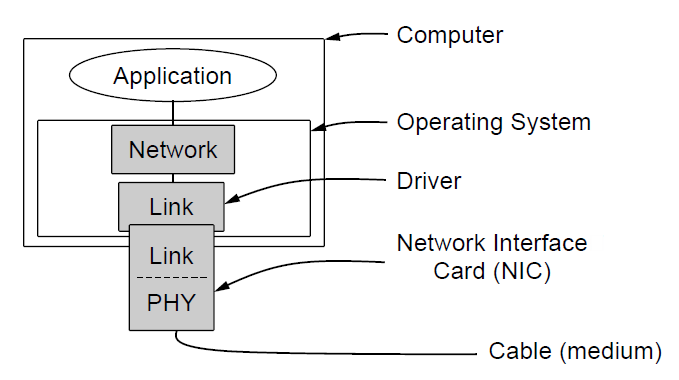
\includegraphics[scale=0.3]{okruzenjeSV}
\end{center}
Komunikacija sloja veze sa ostalim slojevima:
\begin{itemize}
  \item prema mrežnom sloju\\
  Sloj veze dobija od mrežnog sloja sledeći paket, ne može da zahteva neki određen paket i ne može da puta da se traži isti paket. Mora da se obezbede informacije ako se izgube, tj. informacije baferiše pošiljalac.\\
  Kada šaljemo mrežnom sloju paket, samo jednom smemo da šaljemo jedan paket, ne može dva puta da se šalje ako smo pogrešili.
  \item prema fizičkom sloju\\
  Od fizičkog sloja zahtevamo samo jednom jedan okvir. Šaljemo fizičkom sloju samo jednom paket. 
\end{itemize}

Postoje i neki događaji i tajmeri definisani na sloju veze:
\begin{itemize}
  \item wait\textunderscore for\textunderscore event(\&event) - blokirajuća funkcija sve dok se ne dogodi neki event. Čeka na paket/okvir/istek tajmera.
  \item start\textunderscore timer(seq\textunderscore nr) - pokreće tajmer
  \item stop\textunderscore timer(seq\textunderscore nr) - prekida tajmer
  \item start\textunderscore ack\textunderscore timer() - pokreće tajmer za okvir potvrde ACK
  \item stop\textunderscore ack\textunderscore timer() - prekida tajmer za okvir potvrde ACK
\end{itemize}

Protokoli na sloju veze su u\textbf{topijski jednosmerni protokol, „stani i čekaj“ protokol za kanal bez grešaka, „stani i čekaj“ protokol za kanal sa greškama}.
\subsection{Utopijski jednosmerni protokol}
Ovaj protokol ne predviđa pojavu greške, pretpostavlja da su primalac i pošiljalac iste brzine i prenos podataka je jednosmeran.\\

Pošiljalac u beskonačnoj petlji uzima od mrežnog sloja paket po paket i stvara okvir i prosleđuje to fizičkom sloju. Nema mogućnost istovremenog slanja podataka.\\
Primalac u beskonačnoj petlji čeka na događaj. Kad mu stigne događaj (stigao novi okvir) blokirajuća komanda se odblokira. Pretpostavlja se da je okvir validan. Primalac tad iz fizičkog okvira učita okvir i prosledi dalje mrežnom sloju. 
\begin{center}
	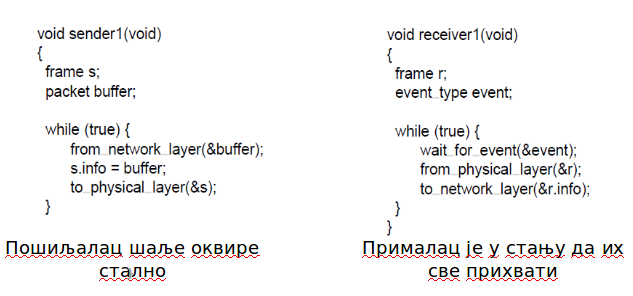
\includegraphics[scale=0.5]{utopijski}
\end{center}
\section{Kontrola toka, ARQ, pauze (tajmauti), duplikati, protokol „stani i čekaj“ za savršen i nesavršen kanal}
(preuzeto iz beleški sa vežbi)\\

Šta ako pošiljalac i primalac nemaju iste brzine slanja, odnosno primanja? Potrebna je kontrola toka.
Kontrola toka je sinhronizacija komunikacije između pošiljaoca i primaoca. Primalac ne sme da bude zatrpan od strane pošiljaoca.\\
\begin{center}
	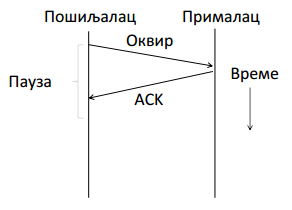
\includegraphics[scale=0.5]{razlBrzine}
\end{center}

\subsection{Protokol „stani i čekaj“ za savršen kanal}
Pretpostavljamo da je kanal savršen, tj. nema grešaka niti izgubljenih okvira i ovaj protokol garantuje usaglašenost u brzini komunikacije. \\
Pošiljalac šalje okvir i čeka potvrdu da je primljen okvir sa druge strane. Ta potvrda znači da je primalac spreman dalje da prima podatke. Primalac kao potrvdu šalje prazan okvir - ack. Šalje se okvir po okvir, što je vrlo neefikasno.
\begin{center}
	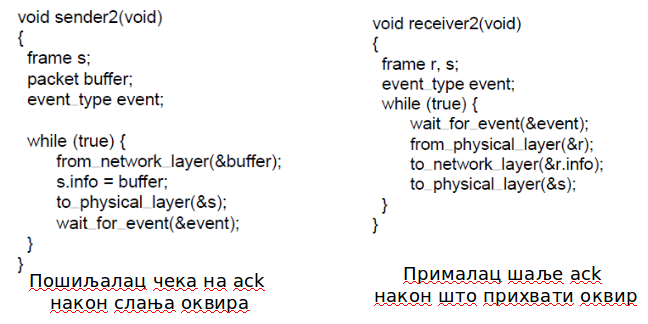
\includegraphics[scale=0.5]{staniIcekaj1}
\end{center}

\subsection{ARQ - Automatic Repeat reQuest}
Šta se dešava ako je nesavršen kanal? Može da se desi da okvir nije stigao na drugu stranu ili da je okvir stigao, ali nije validan i može da se desi da okvir stigne uspešno, ali da se potvrda izgubi. U tom slučaju se radi detekcija i retransmisija ARQ ili korekcija grešaka (obrađeno, više se tiče fizičkog sloja). 
\\
ARQ se obično koristi kada su greške uobičajene i kada se moraju ispraviti, npr. kod WiFi i TCP.\\
Osnovna ideja je da primalac šalje potvrdu o prijemu ispravnog okvira ACK (to je takođe okvir), a pošiljalac uključuje tajmer čim pošalje okvir i automatski šalje ponovo okvir ako istekne vremenska pauza (timeout), osim ako u međuvremenu nije pristigao ACK.
Na sledećoj slici je prikazan scenario sa gubitkom i retransmisijom.
\begin{center}
	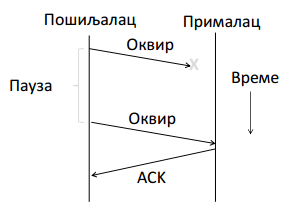
\includegraphics[scale=0.5]{ARQ1}
\end{center}
Osnovni cilj je da okviri budu ispravni i da se ne dupliraju, a sekundarni cilj je da komunikacija bude efikasna.\\

Postavljaju se dva ključna pitanja:
\begin{enumerate}
	\item \textbf{Kolika treba da bude pauza, tj. vreme za koje timeout ističe?}\\
	Pauza ne treba da bude prevelika jer će primalac previše da čeka izgubljene pakete i doći će do neiskorišćenosti kanala. Ne treba da bude ni premala da se ne bi stalno radila retransmisija, odnosno, stalno prekidamo primaoca kada želi da pošalje potvrdu. Dužinu pauze je jednostavno odrediti za LAN (jasna je gornja granica, malo odstupanje), ali je teško za Internet (veliko odstupanje, nema jasne gornje granice).
	\item \textbf{Kako da se izbegne interpretiranje dupliranih okvira kao novih?}\\
	Situacija kada se ACK izgubi dovodi do toga da je moguće interpretirati dupliran okvir kao novi poslati okvir.
\begin{center}
	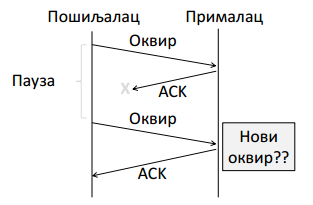
\includegraphics[scale=0.5]{ARQ2}
\end{center}
	Situacija kada je prekratka pauza može da dovede do iste situacije.
\begin{center}
	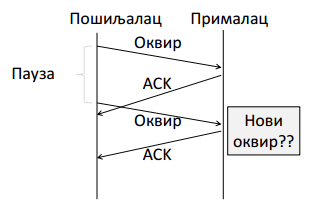
\includegraphics[scale=0.5]{ARQ3}
\end{center}
Iz ovoga izvlačimo da je neophodno da okviri i ACK-ovi nose sa sobom nekakvu oznaku da bi se izbegli duplikati. Dovoljno je da se razlikuje samo trenutni okvir od narednog okvira, što se može predstaviti jednim bitom.
(radi se nekakvo invertovanje bitova, prvi put kad se šalje okvir bit je 0...??)
\end{enumerate}
\subsection{Protokol „stani i čekaj“ za nesavršen kanal}
\begin{center}
	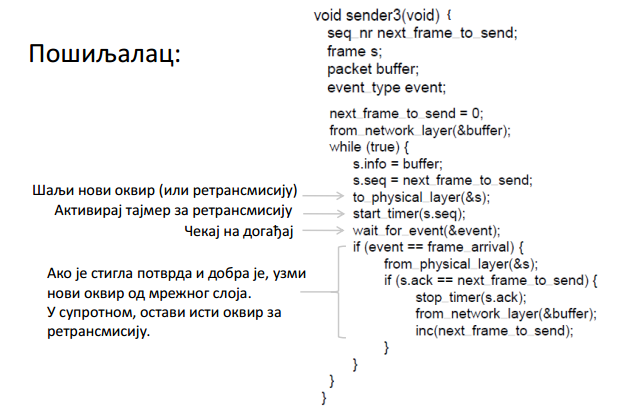
\includegraphics[scale=0.5]{staniIcekaj2}
	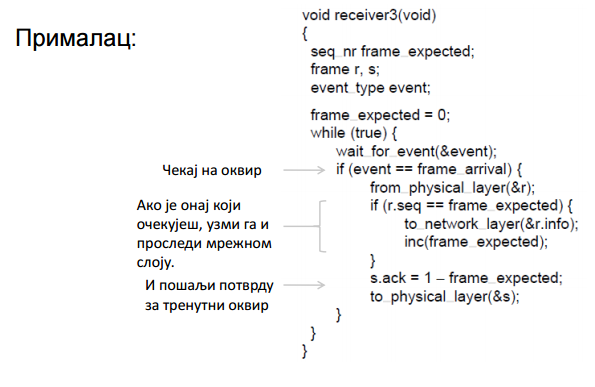
\includegraphics[scale=0.5]{staniIcekaj3}
\end{center}
Ograničenja ovog protokola: 
\begin{itemize}
  \item \textbf{neefikasan}\\
  U datom momentu samo 1 paket prolazi kroz komunikacioni kanal. Prihvatljivo je za LAN, ali vrlo neefikasno za visok BDP. Primer: $B = 1 Mb/s$ $ D=50ms $. Proveriti koliko okvira u sekundi se prenese, i koliko okvira   u sekundi ako je $B = 10 Mb/s$.
\end{itemize}
\section{Protokol kliznih prozora u sloju veze, „1-bitni“, „vrati se N“, „selektivno ponavljanje“}

\subsection{Protokol kliznih prozora u sloju veze}

Uop\v{s}tenje protokola "stani i \v{c}ekaj". Omogu\'{c}ava da u svakom momentu W okvira bude u kanalu. W okvira za RTT (\textit{round trip time} - vreme potrebno da okvir ode i da stigne potvrda za njega).\\
Svakom okviru se dodeljuje redni broj, na osnovu kog se identifikuje. Po\v{s}iljalac i primalac imaju opseg u okviru kog primaju okvire.\\
Po\v{s}iljac ima na raspolaganju W okvira koje mo\v{z}e da po\v{s}alje. Mora da ih baferuje zbog eventualne retransmisije. Sa pristiglim \textit{ack}-ovima po\v{s}iljalac pomera prozor.\\
Primalac ima na raspolaganju prostor za nekoliko okvira koje mo\v{z}e da prihvati. Mora da poseduje bafer za njih. Kako sti\v{z}u novi okviri prozor se pomera.\\
\begin{center}
	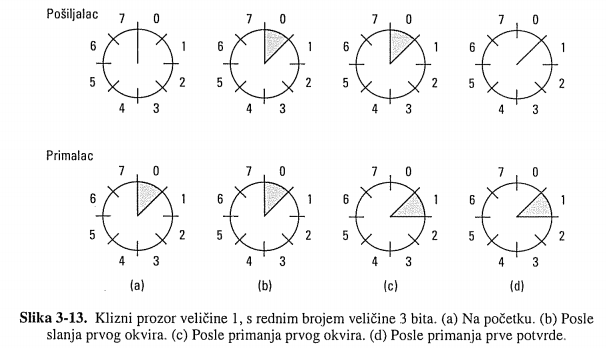
\includegraphics[scale=0.5]{klizni_prozor}
\end{center}
Ve\'{c}i prozori omogu\'{c}avaju proto\v{c}nu odbranu za efikasniju upotrebu kanala. Stani i \v{c}ekaj (W=1) je neefikasan, posebno za du\v{z}e kanale (po\v{s}iljalac \v{s}alje okvir i \v{c}eka potvrdu o prijemu). \v{Z}elim da va\v{z}i $ W \geq{} 2BD + 1 $ u cilju \v{s}to boljeg iskori\v{s}\'{c}enja.

\subsection{"1-bitni"}

Protokol kliznih prozora maksimalne veli\v{c}ine 1. Nema odvojenih algoritama za po\v{s}iljaoca i primaoca, jer sada i jedan i drugi mogu da \v{s}alju i primaju. Za \textit{ack} koristimo okvir iz suprotnog pravca ("\v{s}lepanje").

\begin{center}
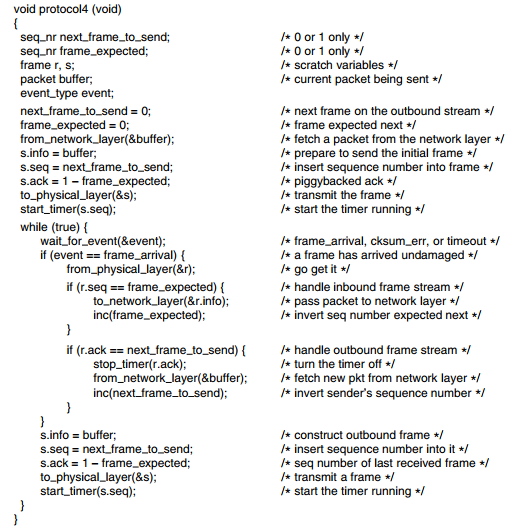
\includegraphics[scale=0.7]{1-bitni-kod}
\end{center}
Ovaj algoritam radi korektno, ali mo\v{z}e do\'{c}i do usporenja ukoliko istovremeno zapo\v{c}nu slanje, jer \'{c}e tako biti izostavljen \textit{ack}, te \'{c}e biti ponovljenih slanja.

\subsection{"Vrati se N"}

Primalac prihvata samo okvire koji sti\v{z}u redom, odbacuje sve koji uslede nakon spornog (okvira koji nije primljen ispravno). Nakon \v{s}to tajmoutuje, ponavljaju se svi nepotvr\dj{}eni okviri do kraja prozora.

\begin{center}
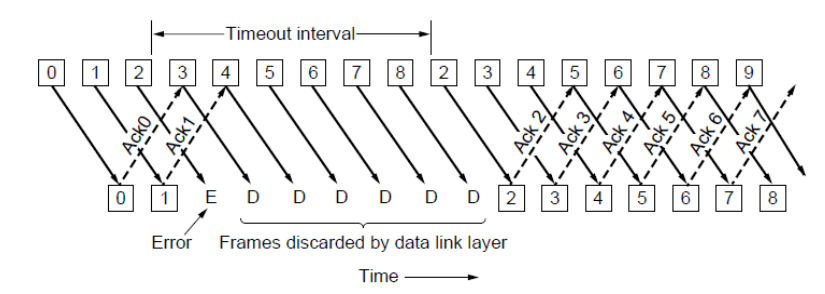
\includegraphics[scale=0.4]{vrati-n}
\end{center}
Jednostavan algoritam na strani primaoca, potreban mu je bafer za samo jedan okvir. Nepotrebno tro\v{s}enje protoka u slu\v{c}aju velikih prozora, u najgorem slu\v{c}aju je potrebno ponoviti slanje celog prozora.

\subsection{"Selektivno ponavljanje"}

Primalac prihvata okvir sve dok je redni broj okvira u opsegu definisanom kliznim prozorom. Negativni \textit{ack} informi\v{s}e po\v{s}iljaoca da ponovo po\v{s}alje problemati\v{c}ni okvir, pre isteka tajmauta za ceo prozor.

\begin{center}
\includegraphics[scale=0.4]{selektivno-ponavljanje}
\end{center}
Slo\v{z}eniji je za implementaciju od "vrati se N" zbog baferisanja pri primanju i vi\v{s}estrukih tajmera pri slanju. Efikasnija upotreba protoka, jer se sada \v{s}alju ponovo samo izgubljeni okviri.\\
Opseg brojeva okvira mora biti barem dva puta ve\'{c}i od veli\v{c}ine prozora kako bi se izbegli problemi sa retransimisijom okvira.

\begin{center}
\includegraphics[scale=0.4]{selektivno-zahtevi}
\end{center}

U prvom slu\v{c}aju, primalac nakon prijema prvih 7 okvira, o\v{c}ekuje okvire 7, 0, 1, 2, 3, 4, i 5, \v{s}to je u konfliktu sa paketima koji su ve\'{c} primljeni. Ako bi po\v{s}iljalac iz nekog razloga ponovio slanje prethodnih paketa, oni bi ponovo bili pogre\v{s}no prihva\'{c}eni i prosle\dj{}eni mre\v{z}nom sloju. U drugom slu\v{c}aju se ovo ne mo\v{z}e desiti.

\section{MAC podsloj, uloga, alokacija kanala, ALOHA protokol}

\subsection{MAC podsloj, uloga}

U svakoj mre\v{z}i u kojoj se koristi neusmereno emitovanje, glavni problem je kako odrediti ko \'{c}e koristiti kanal u situaciji kada ima vi\v{s}e zahteva. Protokoli kojima se odre\dj{}uje slede\'{c}i korisnik takvog kanala pripadaju podsloju sloja veze podataka, poznatom kao podsloj za \textbf{upravljanje pristupom medijumima} (\textit{Medium Access Control, MAC}. Protokol MAC je posebno va\v{z}an za lokalne mre\v{z}e u kojima se za komuniciranje naj\v{c}e\v{s}\'{c}e koristi kanal sa slobodnim pristupanjem.

\subsection{Alokacija kanala}

\begin{enumerate}
	\item Stati\v{c}ko dodeljivanje kanala
	\item Dinami\v{c}ko dodeljivanje kanala
\end{enumerate}

\subsubsection{Stati\v{c}ko dodeljivanje kanala}

Klasi\v{c}an na\v{c}in dodeljivanja jedinstvenog kanala jednom od kandidata na njega je multipleksiranje podelom frekvencije (FDM). Ukoliko postoji $N$ potencijalnih korisnika, propusni opseg se deli na $N$ jednakih delova, po jedan za svakog korisnika. Tako se korisnici ne ometaju me\dj{}usobno. Kada je broj po\v{s}iljalaca veliki ili se stalno menja, tehnika FDM ne zadovoljava. Tako\dj{}e, ako u nekom trenutku \v{z}eli da komunicira manje od $N$ korisnika, veliki deo opsega ostaje neiskori\v{s}\'{c}en. Suprotno, ukoliko vi\v{s}e korisnika \v{z}eli da komunicira, neki od njih nece mo\'{c}i. Drugi metod, sa sli\v{c}nim karakteristikama je TDM (multipleksiranje podelom vremena).

\subsubsection{Dinami\v{c}ko dodeljivanje kanala}

Da bi se razumeo problem, potrebno je sagledati pet osnovnih pretpostavki:
\begin{enumerate}
	\item Model stanica - model sadr\v{z}i $N$ nezavisnih stanica;
	\item Pretpostavka o jedinstvenom kanalu - za sve komunikacije na raspolaganju je jedan kanal;
	\item Pretpostavka o sukobljavanju - ako se dva okvira istovremeno emituju, oni se vremenski preklapaju \v{s}to rezultuje izobli\v{c}enim signalom. Ovaj doga\dj{}aj naziva se \textbf{sukobljavanje};
	\item Vremenski tok:
	\begin{itemize}
		\item Neprekidan vremenski tok - paket se mo\v{z}e poslati u bilo kom trenutku;
		\item Raspore\dj{}eno vreme - vreme podeljeno u intervale odre\dj{}ene veli\v{c}ine, slanje se podudara sa po\v{c}etkom intervala;
	\end{itemize}
	\item Pona\v{s}nje stanica:
	\begin{itemize}
		\item Oslu\v{s}kivanje saobra\'{c}aja na nosiocu podataka - pre upotrebe kanala, stanica mo\v{z}e proveriti da li je slobodan;
		\item Nema oslu\v{s}kivanja saobra\'{c}anja na nosiocu podataka - stanice ne proveravaju da li je kanal prazan, ve\'{c} odmah emituju okvire. Tek kasnije se utvr\dj{}uje da li je prenos uspe\v{s}an.
	\end{itemize}
\end{enumerate}
Za stavke 4 i 5 va\v{z}i jedna od dve postoje\'{c}e mogu\'{c}nosti.

\subsection{ALOHA protokol}

Nastao po ugledu na ra\v{c}unarsku mre\v{z}u koja je povezivala Havajska ostrva '60-ih godina. Postoje dve verzije sistema ALOHA:
\begin{itemize}
	\item \v{C}ista ALOHA
	\item Vremenski raspodeljena ALOHA
\end{itemize}
Kod ALOHA protokola se ne oslu\v{s}kuje saobra\'{c}aj pre slanja.

\subsubsection{\v{C}ista ALOHA}

Po\v{c}iva na jednostavnoj ideji, dozvoliti korisnicima da emituju uvek kada imaju podatke za slanje. Naravno, bi\'{c}e sukobljavanja, ali \'{c}e iz povratnih informacija po\v{s}iljalac jasno videti da je njegov okvir uni\v{s}ten. Kada utvrdi da je poslati okvir o\v{s}te\'{c}en, po\v{s}iljalac \'{c}e slu\v{c}ajno izabran period vremena sa\v{c}ekati eventualnu potvrdu prijema i nakon toga ponovo poslati okvir. Vreme \v{c}ekanja se bira nasumi\v{c}no kako bi se smanjila \v{s}ansa ponovnog sukoba istih paketa.

\begin{center}
	\includegraphics[scale=0.5]{aloha}
\end{center}

Osnovne karakteristike su mu jednostavnost i decentralizovanost. Ovaj algoritam se pokazuje kao prihvatljivo re\v{s}enje kada je malo optere\'{c}enje mre\v{z}e. Me\dj{}utim, algoritam ima lo\v{s}e karakteristike sa uve\'{c}anjem optere\'{c}enja mre\v{z}e. Eksperimentalno utvr\dj{}eno da 18\% okvira pro\dj{}e na drugu stranu.

\subsubsection{Vremenski raspore\dj{}ena ALOHA}

Kod vremenski raspodeljene neophodno je sinhronizovanje globalnog vremena. To se obi\v{c}no posti\v{z}e tako \v{s}to jedna stanica u predodre\dj{}enom intervalu \v{s}alje poseban signal. Time se vreme deli na intervale kona\v{c}ne du\v{z}ine. Emitovanje je dozvoljeno samo na po\v{c}etku intervala. Time se smanjuje verovatno\'{c}a da do\dj{}e do sukoba. Uspe\v{s}nost ovog algoritma je eksperimentalno utvr\dj{}ena i iznosi 36\%.

\section{CSMA, CSMA/CD, BEB}

Kako bi pobolj\v{s}ali karakteristike koje dobijamo sa ALOHA protokolima, koristimo \textbf{protokole za pristupanje uz oslu\v{s}kivanje saobra\'{c}aja na nosiocu podataka} (\textit{carrier sense protocols}). Oslu\v{s}kivanje saobra\'{c}aja ne garantuje da ne\'{c}e biti kolizija zbog ka\v{s}njenja signala.

\subsection{CSMA}

Kada stranica ima podatke za slanje, ona prvo oslu\v{s}ne kanal da bi utvrdila da li je zauzet. Ako na kanalu ima saobra\'{c}aja, stanica \v{c}eka, pa tek kada se kanal oslobodi \v{s}alje svoj okvir. Kada do\dj{}e do sukobljavanja, stranica \v{c}eka tokom nasumi\v{c}no odabranog perioda i po\v{c}inje ponovo. Postoji nekoliko varijacija CSMA protokola:
\begin{itemize}
	\item 1-trajni CSMA - nakon \v{s}to se kanal oslobodi, stanica \v{s}alje okvir sa verovatno\'{c}om jedan \v{c}im utvrdi da je kanal prazan
	\item Povremeni CSMA - kada utvrdi da je kanal zauzet, ne proverava svaki \v{c}as da li se oslobodio, ve\'{c} proverava nakon nasumi\v{c}no odabranog intervala
	\item p-trajni CSMA - ukoliko je kanal prazan, emituje se sa verovatno\'{c}om $p$, dok se sa verovatno\'{c}om $q=1-p$ odustaje od emitovanja do slede\'{c}eg vremenskog intervala
\end{itemize}

\begin{center}
\includegraphics[scale=0.5]{csma}
\end{center}

\subsection{CSMA/CD}

Dodatno pobolj\v{s}anje predstavlja prekid emitovanja ukoliko stanica utvrdi da je do\v{s}lo do kolizije. Time bi se prekinulo ionako bespotrebno slanje izobli\v{c}enih podataka i u\v{s}tedelo vreme i propusni opseg. Ovakav protokol se naziva CSMA uz otkrivanje sukoba (\textit{CSMA with Collision Detection}). Minimalno vreme potrebno za otkrivanje sukoba jednako je vremenu putovanja od jedne stanice do druge, me\dj{}utim, mo\v{z}e se desiti, u najgorem slu\v{c}aju da to vreme bude dvostruko ve\'{c}e. U slu\v{c}aju da najudaljenija stanica po\v{c}ne sa emitovanjem ta\v{c}no u trenutku kad signal prve stigne do nje. U tom slu\v{c}aju \'{c}e informacija o sukobu sti\'{c}i do prve stanice mnogo kasnije. Zbog ovoga se \v{c}esto koristi ograni\v{c}enje za minimalnu du\v{z}inu poruke, kako bi se onemogu\'{c}ilo da stanica po\v{s}alje celu poruku pre nego \v{s}to uo\v{c}i koliziju.  Stanica koja \v{s}alje ne mo\v{z}e primati podatke jer se za oslu\v{s}kivanje kolizije koristi logika primaoca.

\subsection{BEB}

BEB (Binarno Eksponencijalno Odlaganje) protokoli su zapravo modifikacija p-trajnih CSMA protokola (\v{c}esto u kombinaciji sa detekcijom sukobljavanja). Naime, u slu\v{c}aju kolizije \v{c}eka se interval potreban da se po\v{s}alje 0 ili 1 okvir. Tada se ponovo poku\v{s}ava. Ukoliko se ponovo dogodi neuspeh, \v{c}eka se period vremena potreban da se po\v{s}alje izme\dj{}u 0 i 3 okvira. Pri svakom slede\'{c}em neuspehu interval se duplira. Ovako interval brzo raste, i dobija se velika efikasnost u prakti\v{c}noj primeni. Protokol CSMA/CD sa BEB je bio veoma kori\v{s}\'{c}en '80-ih i '90-ih za LAN mre\v{z}e.

\section{MAC protokoli zasnovani na redosledu, Token Ring}

Kako i CSMA daje relativno lo\v{s} rezultate pod visokim optere\'{c}enjem (visoki dodatni tro\v{s}kovi, vreme pristupa varira), potreban nam je protokol koji \'{c}e obezbediti prihvatljive performanse u uslovima visokog optere\'{c}enja.
MAC protokoli zasnovani na redosledu predstavljaju ure\dj{}ene protokole u kojima svaka stanica kada do\dj{}e na red mo\v{z}e da po\v{s}alje okvir ili da propust redosled, ukoliko nema potrebu da \v{s}alje. Ure\dj{}enje se mo\v{z}e definisati po tokenu koji se prosle\dj{}uje ili po vrednosti adrese.

\subsection{Token Ring}

\v{C}vorovi se organizuju u prsten. Token se prosle\dj{}uje u krug. Pravo slanja okvira ima samo \v{c}vor koji poseduje prsten.

\begin{center}
\includegraphics[scale=0.3]{token-ring}
\end{center}

Zajedno sa tokenom, i podaci idu samo u jednom smeru. Ta\v{c}nije, ukoliko stanica primi paket koji nije namenjen njoj, ona ga prosle\dj{}uje dalje u odgovaraju\'{c}em smeru. Ovde treba obezbediti da se paket ne vrti beskona\v{c}no kroz prsten. Uklanjanje paketa iz mre\v{z}e mo\v{z}e obaviti stanica kojoj je paket namenjen ili stanica koja je paket poslala (ukoliko paket obi\dj{}e ceo krug bez da na\dj{}e primaoca).

\subsection{Prednosti i mane}

Kako su svi tro\v{s}kovi unapred predefinisani i onemogu\'{c}ena kolizija, dobijamo efikasniji rad pri visokim optere\'{c}enjima. Tako\dj{}e, garantovano je da \'{c}e u razumnom roku svi (unapred definisanom) svaki \v{c}vor dobiti priliku da po\v{s}alje svoj okvir. Me\dj{}utim, i u ovom protokolu postoje nedostaci. Pre svega, tu je veliki tro\v{s}ak pri malim optere\'{c}enjima. Tako\dj{}e, mo\v{z}e se desiti da se u komunikaciji izgubi token. Ovi protokoli se primenjuju eksperimentalno, kao mogu\'{c}nost pobolj\v{s}anja. Me\dj{}utim, protokoli sa slu\v{c}ajno\v{s}\'{c}u se uglavnom mnogo bolje pokazuju i te\v{s}ko nadma\v{s}uju.

\section{MAC protokoli za bežične mreže}

Be\v{z}i\v{c}na lokalna mre\v{z}a se obi\v{c}no konfiguri\v{s}e unutar poslovne zgrade, pri \v{c}emu se bazne stanice (pristupne ta\v{c}e) razme\v{s}taju na pogodna mesta. Ako se bazne stanice i prenosivi ra\v{c}unari tako podese da emisioni domet bude 3-4m, tada svaka prostorija u zgradi postaje zasebna \'{c}elija, a sama zgrada veliki vi\v{s}e\'{c}elijski sistem (sli\v{c}no kao klasi\v{c}ni sistem mobilne telefonije). Za razliku od telefonije, ovakva \'{c}elija sadr\v{z}i samo jedan kanal koji pokriva \v{c}itav propusni opseg i sve stanice koje se u njoj nalaze. Kada se prijemnik na\dj{}e u dometu dva aktivna predajnika, on prima izobli\v{c}en signal koji je neupotrebljiv.\\
Prvo re\v{s}enje koje se name\'{c}e je upotreba CSMA protokola.

\begin{center}
\includegraphics[scale=0.5]{mac-bezicne}
\end{center}

Na prvoj slici, ukoliko emituje A stanica, stanica C nije svesna toga jer je van dometa i mo\v{z}e tako\dj{}e da krene da emituje. Na ovaj na\v{c}in, stanica B koja je u dometu obe stanice koje emituju, ne\'{c}e biti u mogu\'{c}nosti da primi na ispravan na\v{c}in ni jedan od ova dva signala. Kada stanica ne mo\v{z}e da utvrdi postojanje potencijalnog konkurenta zbog prevelike udaljenosti nastaje \textbf{problem skrivene stanice}. Odavde je o\v{c}igledno da CSMA ne bi bio prihvatljivo re\v{s}enje.

Na drugoj slici, ukoliko stanica B \v{s}alje stanici A neki paket, stanica C koja \v{z}eli da komunicira sa stanicom D bi oslu\v{s}kivanjem zaklju\v{c}ila da je kanal zauzet i odustala bi od slanja, iako njeno slanje ne bi ugrozilo signal koji ide do stanice A. Ovaj problem se naziva \textbf{problem izlo\v{z}ene stanice}. Odavde zaklju\v{c}ujemo da CD ne bi dao prihvatljivo re\v{s}enje. Tako\dj{}e, kod \v{z}i\v{c}ane infrastrukture se mo\v{z}e uo\v{c}iti kolizija i tako prekinuti bespotrebno slanje, \v{c}ime se smanjuje cena. U be\v{z}ni\v{c}noj mre\v{z}i ure\dj{}aji ne mogu da emituju i primaju signal istovremeno, te ne mogu da detektuju koliziju.

Kao re\v{s}enje se name\'{c}e protokol MACA (\textit{Multiple Access With Collision Avoidance} - vi\v{s}ekorisni\v{c}ki pristup sa izbegavanjem sukoba).

\subsection{MACA}

MACA koristi proceduru rukovanja (\textit{handshaking}) umesto CSMA.

\begin{center}
	\includegraphics[scale=0.5]{maca}
\end{center}

Procedura:
\begin{enumerate}
	\item Stanica A \v{s}alje zahtev za slanje (request to send - RTS) stanici B - kratak okvir koji sadr\v{z}i du\v{z}inu okvira sa podacima koji treba da budu poslati naknadno;
	\item Stanica B odgovara dozvolom za slanje (clear to send - CTS) - okvir sadr\v{z}i du\v{z}inu okvira sa podacima (kopirano iz RTS);
	\item Nakon \v{s}to dobije CTS, stanica A emituje okvir.
\end{enumerate}

Za to vreme, ostale stanice koje su dobile RTS znaju da su u dometu stanice koja \v{z}eli da emituje i tako\dj{}e oslu\v{s}kuju i o\v{c}ekuju CTS paket. Ukoliko CTS paket ne stigne do njih, to zna\v{c}i da ne ugro\v{z}ava prenos podataka. Ukoliko stanica primi CTS okvir (bez obzira da li je primila RTS ili ne) zaklju\v{c}uje da se u njenoj blizini nalazi stanica koja treba da primi okvir i primiruje se u toku trajanja prenosa (na osnovu informacija iz CTS).

Na ovaj na\v{c}in je znatno smanjena mogu\'{c}nost pojave kolizije (ne i potpuno uklonjena!). Na primer, vi\v{s}e stanica mo\v{z}e poslati jednoj stanici RTS okvire koji \'{c}e se sukobiti i propasti. U takvoj situaciji, one stanice koje nisu dobile CTS okvir (nakon predvi\dj{}enog vremena), prove\v{s}\'{c}e proizvoljan period u mirovanju i nakon toga ponovo poslati RTS okvir. Za odre\dj{}ivanje ovog intervala se uglavnom koristi BEB.

\section{Klasični Eternet}

\begin{center}
\includegraphics[scale=0.5]{vrsteKablova}
\end{center}

\subsection{10Base5}

Popularno nazvan \textit{tick Ethernet}. Kabl podse\'{c}ao na \v{z}uto ba\v{s}tensko crevo sa oznakama na svakih 2,5m na mestima gde treba ubosti ra\v{c}ve. Veza sa kablom se ostvaruje pomo\'{c}u \textbf{ubodnih ra\v{c}vi} \v{c}ija se igla oprezno utisne u jezgro koaksijalnog kabla. Oznaka 10Base5 ozna\v{c}ava da sistem radi brzinom 10Mb/s, da koristi signaliziranje u osnovnom opsegu i da mo\v{z}e da podr\v{z}i segmente du\v{z}ine do 500m. \textbf{Primopredajnik} je ure\dj{}aj koji se pri\v{c}vr\v{s}\'{c}uje oko kabla tako da njegova ra\v{c}va ostvaruje pouzdan kontakt sa jezgrom kabla. Primopredajnik sadr\v{z}i elektronske komponente pomo\'{c}u kojih oslu\v{s}kuje kabl i otkriva sukobljavanje. Pri detektovanju sukobljavanja, emituje signal ostalim primopredajnicima da bi znali da je do\v{s}lo do sukobljavanja. Spojni kabl (kabl primopredajnika) povezuje primopredajnik sa interfejsom ra\v{c}unara. Mo\v{z}e biti do 50m du\v{z}ine i sadr\v{z}i pet zasebno oklopljenih upredenih parica. Dve parice za prijem i slanje podataka, dve za prijem i slanje signala, a poslednja (koja se ne koristi uvek) slu\v{z}i za napajanje primopredajnika. Neki primopredajnici mogu dopustiti da i do osam ra\v{c}unara bude vezano na njih, time se smanjuje broj potrebnih primopredajnika.

\subsection{10Base2}

Poznat pod nazivom \textit{thin Ethernet}. Umesto ubodnih ra\v{c}vi, koristili su se standardizovani BNC konektori koji formiraju T-spojeve. BNC konektori se lak\v{s}e koriste i pouzdaniji su, oni vr\v{s}e ulogu primopredajnika (svaki ra\v{c}unar mora imato svoj primopredajnik). Ovaj vid kabliranja bio je mnogo jeftiniji i jednostavniji za instalaciju, ali su segmenti kabla mogli da budu najvi\v{s}e 185m dugi i u svakom mo\v{z}e biti najvi\v{s}e 30 ra\v{c}unara.

Kod oba prethodna tipa kabliranja postojao je problem nala\v{z}enja prekida, nesolidno ubodenih ra\v{c}vi i labavih konektora. Zbog toga su razvijane posebne tehnike za otkrivanje gre\v{s}aka. Kroz kabl se pu\v{s}ta impuls i oslu\v{s}kuje se odjek pri nailasku na prepreku ili kraj kabla. Na osnovu dobijenog impulsa se mo\v{z}e lokalizovati uzrok. Tehnika se naziva \textbf{reflektometrija vemenskog domena}.

\subsection{10Base-T}

Zbog te\v{s}ko\'{c}a u vezi sa nala\v{z}enjem mesta prekida u kablu, koristi se vrsta o\v{z}i\v{c}enja gde kablovi iz svih stanica vode u centralni razvodnik (\textbf{hub}), u kom se svi me\dj{}usobno povezuju. Ti kablovi su obi\v{c}no telefonske upredene parice, po\v{s}to obi\v{c}no takvi kablovi ve\'{c} postoje u poslovnim zgradama i ima ih u rezervi. Razvodnici ne baferuju dolazni saobra\'{c}aj. U ovoj konfiguraciji stanice se lak\v{s}e dodaju i uklanjaju, a prekid kabla se lako otkriva. Najve\'{c}a du\v{z}ina kabla mo\v{z}e biti 100m (najvi\v{s}e 200m ukoliko se koriste kvalitetnije parice kategorije 5).

\subsection{10Base-F}

Zasnovan na opti\v{c}kim kablovima. Varijanta je skupa zbog visoke cene konektora i zavr\v{s}nih elemenata, ali je izuzetno imuna na smetnje i preporu\v{c}ljiva je za povezivanje zgrada ili me\dj{}usobno vrlo udaljenih razvodnika. Segment kabla se mo\v{z}e pru\v{z}ati i \v{c}itav kilometar. Sistem je u informacionom smislu bezbedniji, jer je mnogo te\v{z}e prislu\v{s}kivati opti\v{c}ki kabl. 

\subsection{Topologije}

Da bi se ostvarile ve\'{c}e mre\v{z}e, mogu se koristiti \textbf{repetitori} za nadovezivanje segmenta kablova. Repetitor je ure\dj{}aj fizi\v{c}kog sloja koji prima, poja\v{c}ava i ponovo \v{s}alje signal.

\begin{center}
\includegraphics[scale=0.5]{ethernet-topologije}
\end{center}

\begin{itemize}
	\item Linearna topologija - jedan kabl se provla\v{c}i kroz sve prostorije i sve stanice se priklju\v{c}uju u ta\v{c}kama ra\v{c}vanja
	\item Topologija sa okosnicom - od krova do suterena prolazi vertikalni vod od kog se preko specijalnih repetitora granaju horizontalni kablovi (obi\v{c}no vertikalni vod debeo, a horizontalni tanji)
	\item Topologija stabla - naj\v{c}e\v{s}\'{c}e se primenjuje
	\item Segmentirana topologija - najve\'{c}a udaljenost izme\dj{}u dva primopredajnika ne sme biti ve\'{c}a od 2,5km. Izme\dj{}u dva primopredajnika sme biti najvi\v{s}e \v{c}etiri repetitora, predstavlja niz kablovskih segmenata
\end{itemize}

\subsection{MAC protokol podsloja za Eternet}

\begin{center}
\includegraphics[scale=0.5]{format-okvira}
\end{center}

\begin{itemize}
	\item Preambula - 8 bajtova, od kojih svaki sadr\v{z}i sekvencu 10101010 (osim kod poslednjeg bajta, u njemu su poslednja dva bita 11, i on predstavlja oznaku po\v{c}etka okvira - \textit{Start of Frame}). Slu\v{z}i za sinhronizaciju primaoca sa po\v{s}iljaocem.
	\item Adrese odredi\v{s}ta i izvori\v{s}ta - najzna\v{c}ajniji bit prve adrese mo\v{z}e biti
	\begin{itemize}
		\item 0 - obi\v{c}ne adrese
		\item 1 - grupne adrese
	\end{itemize}
	\item Tip - saop\v{s}tava primaocu \v{s}ta da radi sa okvirom, odnosno, kom protokolu mre\v{z}nog sloja treba proslediti okvir
	\item Podaci - polje du\v{z}ine do 1500 bajtova, u Ethernet protokolu okvir mora biti najmanje 64 bajta zbog eventualnog naglog prekida i potencijalnih sukoba, te ako je ovo polje manje od 46 bajtova, dopunjuje se u polju Dopuna.
	\item Kontrolni zbir - 32-bitni klju\v{c} za he\v{s}iranje podataka, CRC
\end{itemize}

\section{Moderni (komutirani) Eternet}

Sa pove\'{c}anjem broja stanica, saobra\'{c}aj postaje sve gu\v{s}\'{c}i. Da bi se prevazi\v{s}lo zasi\'{c}enje mre\v{z}e mo\v{z}e se pove\'{c}ati brzina prenosa (sa 10Mb/s na 100Mb/s). Me\dj{}utim, kada uzmemo u obzir tempo razvoja, lako se mogu zasititi i gigabitne mre\v{z}e. Drugi na\v{c}in je kori\v{s}\'{c}enje komutiranog Etherneta. Jezgro takvog ure\dj{}aja je \textbf{skretnica} (\textit{switch}) koja na brzoj osnovnoj plo\v{c}i naj\v{c}e\v{s}\'{c}e ima mesta za 4 do 32 linijske kartice, od kojih svaka sadr\v{z}i jedan do osam konektora. Svaki konektor povezuje jedan umre\v{z}eni ra\v{c}unar preko upredene parice i spoja 10Base-T. Kod razvodnika (\textbf{hub}) smo imali situaciju da se ulaz ponavlja na svim izlazima.

\begin{center}
\includegraphics[scale=0.5]{hub-switch}
\end{center}

Kako switch radi na sloju veze, on koristi adrese iz okvira i na taj na\v{c}in prosle\dj{}uje okvir na odgovaraju\'{c}i izlaz, bez znanja ostalih izlaza o postojanju okvira. Svaki izlaz switch-a je odvojen kolizioni domen, za razliku od hub-a, kod kog se kolizioni domeni ne dele. Zbog podele kolizionih domena, vi\v{s}e ne mo\v{z}e do\'{c}i do kolizije i CSMA/CD nije potreban. Me\dj{}utim, kako vi\v{s}e stanica mo\v{z}e poslati istovremeno okvir na isti izlaz, neophodno je da u switch-u postoji bafer u koji \'{c}e se sme\v{s}tati okvir dok se ne rastereti saobra\'{c}aj.

Uvo\dj{}enjem switch-eva i hub-ova je zamenjen koncept deljenih kablova koji je bio aktivan ranije. Sa ovim pristupom je znatno jednostavnije dodati novi ure\dj{}aj, a dobija se i na pouzdanosti (lak\v{s}e se nalazi kvar). Switch omogu\'{c}ava pove\'{c}an protok, odnosno svaka linija ima pun kapacitet. Tako\dj{}e, topologija mre\v{z}e po\v{c}ela da li\v{c}i na zvezdu.

Neophodno je da switch na ispravan izlaz prosledi dobijen okvir. Metod koji se primenjuje naziva se u\v{s}enje unazad. Pravi se tabela relacija broja porta (izlaza) i adrese koja se nalazi na tom portu. Tabelu popunjavamo posmatranjem portova i adresa stanica koje \v{s}alju okvire. Kada se prosle\dj{}uje okvir, ukoliko postoji unos u tabeli \v{s}alje se okvir samo na taj port, u suprotnom se okvir prosle\dj{}uje na sve portove.

U mre\v{z}i se mogu vi\v{s}estruko upotrebljavati switch-evi i hub-ovi, sve dok se ne pojavljuju petlje. U slu\v{c}aju ovakvih mre\v{z}a, nekim portovima \'{c}e biti dodeljeno vi\v{s}e adresa.

\begin{center}
\includegraphics[scale=0.3]{visestruki-hub-switch}
\end{center}

Ukoliko se u mre\v{z}i javljaju petlje (\v{c}esto se namerno projektuju da imaju redundantnost), potrebno je petlje otkloniti kako bi dobili funkcionalnu mre\v{z}u. To se posti\v{z}e formiranjem razapinju\'{c}eg stabla (u dubinu ili u \v{s}irinu).

\section{Mrežni sloj, uloga, motivacija, rutiranje i prosleđivanje (ukratko), tipovi servisa na mrežnom sloju, objašnjenja i njihov uporedni odnos}

\subsection{Mre\v{z}ni sloj, uloga, motivacija, rutiranje i prosle\dj{}ivanje}

Sa slojem veze mi smo ve\'{c} dobili funkcionalnu mre\v{z}u. Problem sa pristupom sloja veze je \v{s}to bi u tom slu\v{c}aju bilo neophodno pamtiti ogromnu tabelu relacija i \v{s}to bi se inicijalna poruka slala celom svetu. Zbog prirode switch ure\dj{}aja je nemogu\'{c}e da se koriste razli\v{c}ite tehnologije u razli\v{c}itim delovima mre\v{z}e. Jo\v{s} jedan nedostatak je na\v{s}a potreba da imamo kontrolu mre\v{z}nog saobra\'{c}aja, odnosno da odre\dj{}ujemo rute (putanje) kojim \'{c}e paket stizati od jedne do druge ta\v{c}ke.

Zadatak mre\v{z}nog sloja je da pakete od izvori\v{s}ta sprovede celim putem do odredi\v{s}ta, \v{s}to zna\v{c}i da treba da ih provu\v{c}e kroz brojne usputne usmeriva\v{c}e (rutere). \textbf{Rutiranje} je proces odlu\v{c}ivanja u kom pravcu treba poslati saobra\'{c}aj. Da bi ostvario ovaj zadatak, mre\v{z}ni sloj mora da poznaje topologiju komunikacione podmre\v{z}e i da kroz njih bira odgovaraju\'{c}e putanje. Njegov zadatak je i da vodi ra\v{c}una da se neke linije i ruteri ne preopterete (algoritmi nad grafovima). \textbf{Prosle\dj{}ivanje} je proces slanja paketa na osnovu lokalne tabele, pretpostavlja se da je pre prosle\dj{}ivanja obavljeno rutiranje.

\subsection{Tipovi servisa na mre\v{z}nom sloju}

Postoje dva tipa mre\v{z}nih servisa:
\begin{itemize}
	\item Datagram - servisi bez uspostavljanja veze (poput po\v{s}te)
	\item Virtuelna kola - servisi sa uspostavljanjem veze (poput fiksne telefonije)
\end{itemize}

Oba tipa se realizuju tehnikom sa\v{c}uvaj-i-prosledi (\textit{store-and-forward}. Ova tehnika je vrlo jednostavna, nakon \v{s}to ruter dobije paket, privremeno ga \v{c}uva (baferi\v{s}e), sve dok ne bude u mogu\'{c}nosti da ga prosledi dalje. Koristi se tehnika statisti\v{c}kog multipleksiranja za upravljanje protokom.

Kod datagramskih servisa, paket sadr\v{z}i ciljnu adresu na osnovu koje ruter prosle\dj{}uje paket dalje

\begin{center}
\includegraphics[scale=0.5]{datagramski-servis}
\end{center}

Svaki ruter sadr\v{z}i tabelu prosle\dj{}ivanja (\textit{forwarding table}), u kojoj za svaku adresu postoji susedni \v{c}vor na koji se paket namenjen toj adresi prosle\dj{}uje (slede\'{c}i hop). Ova tabela se tokom vremena mo\v{z}e menjati, u zavisnosti od algoritma za usmeravanje koji se primenjuje. Za ozna\v{c}avanje stanica se koristi IP adresa (32-bitna identifikacija), u okviru IPv4 paketa \v{c}ija je maksimalna veli\v{c}ina oko 1,5KB, sadr\v{z}i (osim adrese) i verziju, zaglavlje, du\v{z}inu paketa, kontrolni zbir...

Kako se ne bi za svaki paket izmi\v{s}ljala nova putanja koriste se virtuelna kola. Na ovaj na\v{c}in, jednom uspostavljena putanja od izvori\v{s}ta do odredi\v{s}ta se ne menja i postaje parametar koji se unosi u tabelu. Kada se veza raskine, raskine se i odgovaraju\'{c}e virtuelno kolo. Svaki paket sa sobom nosi identifikator virtuelnog kola kom pripada.

\begin{center}
\includegraphics[scale=0.5]{virtuelno-kolo}
\end{center}

Identifikator virtuelnog kola nema globalno zna\v{c}enje, poput IP adrese, ve\'{c} se koristi samo na nekom delu sloja veze.

Oba pristupa imaju svoje prednosti i mane, u skladu sa slede\'{c}om tabelom:

\begin{center}
\includegraphics[scale=0.5]{datagrami-vk}
\end{center}

Kada \v{z}elimo da pove\v{z}emo datagramske servise i virtuelna kola, neophodno je preslikavanje izme\dj{}u IP adresa i identifikatora virtuelnog kola. Provajderi \v{c}esto koriste virtuelna kola kako bi grupisali IP saobra\'{c}aj i br\v{z}e ga preneli.

\begin{center}
\includegraphics[scale=0.3]{datagrami-vk-kombinacija}
\end{center}

\section{IP adrese i prefiksi}
Internet se u mreznom sloju moze posmatrati kao skup medjusobno povezanih podmreza ili autonomnih sistema. Kombinovana mreza nema odredjenu strukturu , osim veceg broja velikih okosnica koje se sastoje od linija velike propusne moci I brzih usmerivaca. Na okosnice su prikljucene regionalne mreze ,a za njih se vezuju lokalne mreze univerziteta, kompanija I davalaca Internet uluga.\\

\begin{center}
\includegraphics[width=12cm, height=6cm]{okosnica}\\
\end{center}
Citav Internet na okupu drzi protokol mreznog sloja tzv. \textbf{Protokol IP}. Njegov zadatak je da na najbolji moguci nacin obezbedi prenos datagrama od izvorista do odredista, bez obzira da li se racunari nalaze na istoj mrezi ili se I druge mreze nalaze izmedju njih.\\

Na Internetu se komunicira na sledeci nacin. Transportni sloj preuzima tokove podataka I deli ih u datagrame. Svaki datagram se prenosi Internetom I mozda usput deli I na  manje fragmente. Mrezni sloj od njih sklapa originalni datagram, kad svi delovi stignu. Zatim se taj datagram predaje transportnom sloju koji ga umece u ulazni tok procesa za prihvatanje podataka kod primaoca.\\

IP datagram sadrzi zaglavlje (fiksni deo duzine 20 bajtova I opcioni deo promenljive duzine) I tekstualni deo. Format zaglavlja prikazan na slici ispod. Ono se prenosi redosledom  “big-endian” sleva udesno, pri cemu prvo ide najznacajniji bit polja Verzija (tu je oznacena verzija protokola kome pripada datagram), zatim IHL (Internet header length) belezi se duzina zagavlja u 32-bitnim recima, vrsta usluge, ukupna duzina, identifikacija (odredisni racunar odredjuje kom  datagramu pripada pristigli fragment), redni broj fragmenta, zivotni vek (ogranicava trajanje paketa na mrezi), protokol (proces kome paket treba predati, taj proces moze biti protokol TCP, UDP…), kontrolni zbir zaglavlja(koristi se za proveru gresaka izazvanih neispravnim memorijskim recima usmerivaca . Algoritam radi tako sto se aritmetikom nepotpunih komplemenata sabiraju sve 16-bitne polureci onako kako pristizu, a zatim se od rezultata odbije nepotpuni komplement. Jednak nuli ako nema greske), izvorisna adresa I odredisna adresa ukazuju na broj mreze I broj racunara, opcije.
\subsection{IP adrese}
Citava Internet na okupu drzi protokol mreznog sloja, tzv. protokol IP.
Svaki racunar i svaki usmeravac na Internetu imaju svoju IP adresu koja obuhvata broj njihove mreze i broj racunara. Ta komb. je jednistvena, dva racunara u nacelu ne mogu imati istu IP adresu. IP adresa se ne odnosi na racunar,  vec na mrezni interfejs, pa ako se racunar nalazi u dve mreze, mora imati dve IP adrese. Koriste se u poljima izvorisna adresa I odredisna adresa. \\

Vec vise decenija IP adrese se dele u pet kategorija, prikazanih na slici:
 \begin{center}
\includegraphics[width=12cm, height=6cm]{klasnoAdr}\\
\end{center}
 Takva podela se naziva klasno adresiranje. Vise se ne koristi. Da bi se izbegli sukobi, brojevi mreza dodeljuje neprofitna \textbf{Korporacija za dodeljivanje imena i brojeva na Internetu (ICANN)}.
IPv4 adresa koristi 32-bitnu adresu, a  IPv6 koristi 128-bitnu adresu.\\

Notacija u vidu kvarteta dekadnih brojeva:\\
 - cetiri 8-bitna broja odvojena tackama – svaka od 4 bajta pise se decimalno 
 \begin{center}
\includegraphics[width=12cm, height=3cm]{IPadresa}\\
\end{center}
Adresu 0.0.0.0 koriste racunari u fazi ukljucivanja. IP adresa s mreznim brojem 0 oznacava tekucu mrezu. Takve adrese omogucavaju racunarima da adresiraju sopstvene mreze iako joj ne znaju broj. Adresa koja se sastoji samo od jedinica omogucava neusmereno emitovanje u lokalnoj mrezi.
 \begin{center}
\includegraphics[width=12cm, height=6cm]{specijalneIP}\\
\end{center}

\subsection{Prefiksi}
IP adrese su hijerarhijski, za razliku od Ethernet adrese. Svaka 32-bitna adresa
se sastoji od mreznog dela promenljive dužine (gornji bitovi) i dela Host
(donji bitovi). mrezni deo ima istu vrednost za sve Host delove na jednoj
mreži, kao što je Ethernet LAN. \\

Adrese se grupisu u blokove koje se nazivaju \textbf{prefiksi}.
\begin{itemize}
  \item \textbf{L-bitni prefiks} je grupa adresa koje imaju isti prefiks duzine L bita
 \item to znaci da L-bitni prefiks ima $2^{32-L}$ razlicitih adresa
prefiksi opisuju mreze racunara odnose opsege adresa 
 \item Prefiksi se pisu zadavanjem najnize IP adrese u bloku i velicine bloka.
\end{itemize}
 \begin{center}
\includegraphics[width=12cm, height=3cm]{prefiks}\\
\end{center}
Notacija olika "IP adresa/duzina prefiksa"\\
\begin{itemize}
  \item npr. 128.13.0.0/16 je opseg 128.13.0.0. do 128.13.255.255
  \item prefiks oblika /24 odgovara opsegu sa 256 adresa dok /32 odgovara jedinstvenoj adresi\\
 adresa pripada razlicitim prefiksima
 \begin{center}
\includegraphics[width=12cm, height=3cm]{prefiks2}\\
\end{center}
\item \textbf{vise sprecifican prefiks} je duzi prefiks jer blize odredjuje opseg oko te adrese
\item \textbf{manje sprecifican prefiks} je kraci prefiks . KOji je najmanje sprecifican?
\begin{center}
\includegraphics[width=12cm, height=3cm]{prefiks3}\\
\end{center}
\end{itemize}

\subsection{IP klase adresa - stari sistem grupisanja}

 Ranije su IP adrrse bile grupisane u klase adresa fiksne duzine.\\
Klasa C je npr. adekvatna za lokalne mreze 
\begin{center}
\includegraphics[width=12cm, height=3cm]{ranije}\\
\end{center}
\subsection{Javne/ privatne IP adrese}
Javna IP adresa npr. 18.31.0.1
\begin{itemize}
  \item jedinstvena oznaka racunara na Internetu
\item mora se dodeliti pre upotrebe (regularno telo)
\item vecim delom potrosene... dolazi vvreme za prelazak na IPv6
\end{itemize}
Privatne IP adrese
\begin{itemize}
  \item nisu globalno jednistvene
\item jesu jednistvene na novou manjih mreza, npr. u mrezi firme, kucne lokalne mreze..
\item primeri: 10.0.0.0/8, 192.168.0.0/16
\item potrebna je javna bar jedna javna IP adresa i NAT da bi se iz ovakvih mreza povezali na Internet
\end{itemize}
\subsection{Dodeljivanje javnih IP adresa}
Hijerarhijski proces
\begin{itemize}
  \item IANA je svetsko regulatorno telo  - dodeljuje ceo opseg adresa reg. telima
\item Regionala tela dodeljuju osege kompanijama u regionu
\item Kompanije dodeljuju konkretnim racunarima
 \begin{center}
\includegraphics[width=12cm, height=3cm]{IANA}
\end{center}
\end{itemize}

Kljucna prednost prefiksa je da ruteri mogu proslediti pakete na osnovu samo
mreznog dela adrese. Deo Host nije bitan ruteru jer su svi Host ista mreža pa  ce bitii poslani u istom pravcu. Kad se paketi dostave mrezi, tek tada ce biti usmereni ka ciljnom Hostu.\\

Ovo čini matrice tabele mnogo manje nego što bi inače
bila.  Uzmite u obzir da je broj Hostova na Internetu priblizno jednu milijardu.
To bi bio veoma velika tabela za svaki ruter. Medjutim, koristecci
hijerarhija, ruteri treba da zadrži rute za samo oko 300.000 prefiksa.
\subsection{Podmreze}
Svi racunari na istoj mrezi moraju imati isti mrezni broj. To pravilo IP adresiranja moze da stvori probleme tokom rasta mreze. Resenje je nadjeno u tome da se mreza interno podeli na vise delova, ali da za spoljni svet ostane celovita.\\
 
U literaturi o Internetu, delovi mreze zovu se \textbf{podmreze}.\\

Kada paket stigne u glavni usmerivac, kako ovaj zna na koju podmrezu da ga postavi? Glavni usmerivac bi mogao da ima tabelu sa 65.536 odrednica za svaki racunar/usmerivac na univerzitetu. To bi radilo, ali tabela bi bila prevelika i trebalo bi je cesto ruucno odrzavati. Zato se u praksi primenjuje druga sema. Umesto da se zadrzi jednistvena adresa klase B sa 14 bitova za mrezu i 16 bitova za racunar, od racunarskih bitova se jedan deo uzima za oznacavanje podmreze. Na primer, koristi se 6-bitni broj za podmreze i 10-bitni broj za racunare. Da bi se ugradile podmreze, glavni usmerivac treba da ima masku podmreze koja naznacava podelu adrese izmedju mreze + podmreze i racunara. Maska podmreze se takodje pise decimalnom notacijom s tackom, s tim sto se bitovi koji znacavaju mrezu i podmrezu razdvajaju kosom crtom od bitova koji oznacavaju racunar. 
 \begin{center}
\includegraphics[width=12cm, height=4cm]{maskaPodmreze}\\
\end{center}

\section{IP prosleđivanje}
\begin{itemize}
  \item Sve IP adrese jedne mreze pripadaju istom prefiksu
\item Svaki usmerivac poseduje tabelu uredjenih parova oblika (prefiks, sledeci cvor - hop)
\item Zasto ne (ciljna adresa, sledeci cvor)?
 \begin{center}
\includegraphics[width=12cm, height=4cm]{prosledjivanje}\\
\end{center}
\end{itemize}
Niko ne zna koliko mreze je  povezano sa Internetom vise, ali to je veliki broj, verovatno najmanje milion. Ovo moze biti veoma veliki tabela. To mozda ne zvuči velika prema racunarskim standardima, ali treba imati u vidu  da ruteri moraju pretraziti ovu  tabeli da bi prosledili svaki paket.  Samo fizicko skladistenje ovakve tabele je izvodljivo, premda skupo resenje za kriticne rutere koji tabele cuvaju u statickom RAM-u na ulazno-izlaznim kartcama. Ozbiljniji problem je sto slozenost raznih algoritama koji rade s tabelama ne rasste linearno s duzinom tabele vec brze. Osim toga, neki algoritmi za usmeravanje zahtevaju da svaki ruter povremeno emituje svoju tabelu, pa moze doci do toga da se neki deo usput izgubi I na taj nacin se onemogucava dobijanje potpunih podataka. \\

Problem tabele za usmeravanje mogao bi se resiti produzavanjem hijerarhije, tj. Kada bi  , na primer, svaka IP adresa sadrzala polje za drzavu, pokrajinu, grad, mrezu, racunar . Tada bi svaki ruter jedino mora da zna kako da podatke isporuci svakoj stranoj drzavi, pokrajini u svojoj zemlji, gradovima u tim pokrajinama, mrezama u tim gradovima. To bi zahtevalo IP adresu mnogo duzu od 32 bita I neefikasno bi koristila adresni proctor.\\

Resenje koje je realizovano I koje je Interentu omogucilo da za neko vreme predahne zove se besklasno medjudomensko usmeravanje (CIDR). \\
Osnovna zamisao je bila da se preostali nedodeljen adresni proctor podeli u blokove razlicite velicine, ne vodeci racuna o klasama.\\
Sa sistemom CIDR, svaka ciljna tabela za usmeravanje prosiruje se 32-bitnom maskom - prefiksom. Tako nastaje jedinstvena tabela usmeravanja za sve mreze, koja se sastoji od niza tripleta, IP adresa, prefiks, izlazna linija. Kada paket stigne , najpre se iz njega izvlaci IP adresa. Zatim se tabela usmeravanja pregleda, maskiranjem ciljne adrese I poredjenjem sa ciljnim adresama u tabeli da bi se pronasal odgovarajuca. Ako se nadje vise odgovarajucih ciljnih adresa koje se razlikuju samo po duzini prefiksa, koristi se ona sa najduzim prefiksom. Na primer, ako se sa ciljnom adresom slazu adrese sa prefiksom /20 I /24, izabrati onu a prefiksom /24. 
 \begin{center}
\includegraphics[width=12cm, height=4cm]{najduziPrefiks}\\
\end{center}
Sa slajda:
\begin{itemize}
  \item prefiksi u tabeli se mogu preklapati!
\item Pravilo najduzeg odg. prefiksa:\\
1. Za svaki paket, pronadji najduzi prefiks koji sadrzi ciljnu adresu, odnosno najspecificniji prefiks\\
2. Poslediti paket cvoru koji odgovara tom prefiksu 
   \begin{center}
\includegraphics[width=12cm, height=4cm]{najduziPrefiks1}\\
\end{center}

\end{itemize}
Primer sa prefiksom:
 \begin{center}
\includegraphics[width=12cm, height=12cm]{primerPrefiks1}\\
\end{center}
 \begin{center}
\includegraphics[width=12cm, height=12cm]{primerPrefiks2}\\
\end{center}
 \begin{center}
\includegraphics[width=10cm, height=5cm]{primerPrefiks3}\\
\end{center}

\section{ARP i DHCP}
\subsection{ARC protokol za razresavanje adresa}
ako svaki racunar na Internetu ima jednu (ili vise) IP adresa, one se u stvari ne mogu koristiti za slanje paketa jer hardver sloja veze podataka ne razume Internet adrese. Danas su racunari u vecini kompanija I univerziteta povezani u lokalne mreze preko mrezne kartice koja razume samo lokalne adrese. Na primer, Ethernet kartice oduvek imaju ugradjenu 48-bitnu Ethernet adresu. Proizvodjaci Ethernet katica zahtevaju od centralne ovlascene organizacije da im dodeli blok adresa kako bi svaka kartica imala jedinstvenu adresu. Kartice salju I primaju okvire zasnovane na 48-bitnim Ethernet adresama. One ne znaju nista o 32-bitnim IP adresama.\\

Sada se postavlja pitanje: kako se IP adrese preslikavaju u adrese sloja veze podataka, npr. U Ethernet adrese, tj. Kako cvor, na osnovu ciljne IP adrese, da se sazna adresu u sloju veze kako bi poslao okvire na odgovarajuci cvor?
 \begin{center}
\includegraphics[width=10cm, height=3cm]{slojVeze}\\
\end{center}
Opis protokola(jenostavan):\\
1. Cvor koji hoce da sazna emituje ID adresu\\
2. Onaj koji ima tu adresu za svoju izvornu, vraca mu odgovor sa svojom adresom u sloju veze
 \begin{center}
\includegraphics[width=10cm, height=4cm]{arp}\\
\end{center}
Primer sa univerzitetom
Imamo mali univerzitet kojim ima nekoliko mreza klasa C(sada zvanih /24), tu imamo 2 Ethernet mreze, jednu sa IP adresom 191.31.65.0 I drugu  sa IP adresom 191.31.63.0. Svaki racunar na Ethernet mrezi ima jedinstvenu Ethernet adresu, oznacenu sa E1 do E6. Racunar 1 difuzno emituje paket na Ethernet pitajuci : Ko ima IP adresu 192.31.65.5? Pitanje ce stici do svakog racunara na Ethernet mrezi 192.31.65.0 I svaki ce proveriti svoju IP adresu. Samo ce racunar2 odgovoriti sa svojom Ethernet adresom (E2). Protokol kojim se ovakovo pitanje salje I na njega dobija odgovor se naziva protokol za razresavanje adresa.
 \begin{center}
\includegraphics[width=12cm, height=15cm]{primerARP}\\
\end{center}
Prednost ovog protokola je jednostavnost njegovog koriscenja. Administratop sistema treba svakom racunara da dodeli IP adresu I odluci o prefiksu(bloku mreze), sve ostalo radi ARP.\\
U ovoj fazi, IP softver na racunaru1 pravi Ethernet okvir adresiran na E2, smesta IP paket u polje za korisnicke podatke I salje na Ethernet. Ethernet kartica racunara2 otkriva ovaj okvir.\\
Jedna od optimizacija bi bila da racunar koji izvrsi protokol ARP cuva rezultat za slucaj da uskoro treba da ponovo stupi u vezi sa istim racunarom (pronadje uparene adrese u sopstvenom kesu).
\subsection{DHCP Protokol za dinamicko podesavanje racunara}
Javlja se problem dodeljivanja IP adrese u mrezi. Tek podignuti cvor trazi svoju IP adresu. Postavlja se pitanje: koja je njegova IP adresa, koja je IP adresa njegovog usmerivaca itd.\\
Ethernet adresa se fabricki zadaje, ali IP adresa ne.
 \begin{center}
\includegraphics[width=8cm, height=3cm]{dhcp}\\
\end{center}
Protokol DHCP omogucava I rucno I automatski dodeljivanje IP adresa. Protokol DHCP se oslanja na specijalan server koji dodeljuje IP adrese onim racunarima koji ih trazi. Taj server ne mora da bude na istoj lokalnoj strani kao I racunar koji zahteva adresu. \\
Sa DHCP, svaka mreza mora da ima DHCP server koji je ogovoran za konfiguraciju.\\
1. Cvor emituje paket (DISCOVER package, koji mora da dodje do DHCP servera) celoj mrezi (specijalana adresa za emitovanje je 255.255.255.255) \\
2. DHCP odgovara cvoru ciljano na osnovu MAC adrese sa predlozenom IP adresom u okviru OFFER package\\
3. Cvor emituje odgovor da mu odgovara predlozena adresa (moze da bude vise DHCP-ova)\\
4. DHCP potvrdjuje I brise adresu iz spiska slobodnih IP adresa
 \begin{center}
\includegraphics[width=8cm, height=3cm]{dhcp2}\\
\end{center}
Klijent moze I da obnovi vec dodeljenu IP adresu ako je ranije dobio, salje samo REQUEST I dobija ACK.\\
Protokol takodje omogucava paralelan rad vise repliciranih DHCP servera :
zarad pouzdanosti I efikasnosti i REQUEST se emituje tako da su sinhronizovani\\
Pitanje koje se namece sa automatskim dodeljivanje IP adrese iz zajednickog skladista koliko dugo IP adresa treba da bude dodeljena. Ako se racunar iskljuci sa  mreze i ne vrati svoju IP adresu DHCP serveru, ona se nepovratno gubi. Posle nekog vremena, mnoge adrese mogu biti izgubljena. Da bi se  sprečilo to, dodeljivanje IP adresa se dodeljuju na određeni vremenski period, tehnika se zove iznajmljivanje(eng.leasing). Neposredno pre isteka zakupa, racunar mora da traži DHCP obnovljanje najma. Ako to ne ucini ili zahtev bude odbijen, racunar ne  moze  više ne koriste tu IP adresu.
\section{ICMP i NAT}
IPv4 omogucava samo par milijardi dostupnih javnih adresa, medjutim racunara koji se povezuju na Internet je mnogo vise. Dugorocno resenje bi bilo da citav Internet predje na protokol IPv6 sa 128-bitnim adresama. Taj proces jeste u toku, ali ce proci godine pre nego sto se dovrsi. Zbog toga su mnogi osetili potrebu za nekim brzim resenjem. Ono se pojavilo u obliku sistema za prevodjenje mreznih adresa (NAT). NAT povezuje racunare iz lokalne mreze na spoljnu adresu , npr. Internet.\\
\begin{enumerate}
	\item Kucni racunari koriste “private” IP adrese (sluze za interni saobracaj).
	\item NAT (u okviru kucnog usmerivaca -AP) povezuje vise kucnih racunara na jednu javnu adresu (sluzi za saobracaj na 			Internetu) dodeljenu od strane ISP.
	Kada paket napusta lokalnu  mrezu I odlazi ka davaocu Internet usluga, njegova adresa se prevodi. Da bi takav sistem
	mogao da radi, tri opsega IP adresa rezervisana su za private potrebe, s tim da se paketi s tim adresama ne smeju
	pojaviti na Internetu, a mogu se interno koristiti kako god zele. Tri rezervisana opsega su:
	\begin{center}
		\includegraphics[width=9cm, height=5cm]{opseg}\\
		\includegraphics[width=9cm, height=5cm]{nat}\\
	\end{center}
\end{enumerate}
Kako NAT radi?
\begin{enumerate}
	\item On podrzava tabelu (preslikavanje) unutrasnjih/spoljnih adresa
	\item Zapravo je to preslikavanje IP+TCP port informacija 
	\begin{center}
		\includegraphics[width=9cm, height=5cm]{preslikavanje}\\
	\end{center}
	\item Portovi su neophodni kaako bi mapiranje bilo 1-1, jer je spoljnih adresa manje (obicno samo jedna)
	\begin{enumerate}
		\item Prilikom slanja podataka iz lokalne mreze 
			\begin{enumerate}
				\item Svakom IP paketu se menja adresa posiljaoca u skladu sa zadatim preslikavanjem (s leva na desno)
			\end{enumerate}
		\item Prilikom prihvataja podataka iz spoljne mreze
		\begin{enumerate}
			\item Svakom IP paketu se menja adresa primaova u skladu sa zadatim preslikavanjem (s desna na levo)
		\end{enumerate}
	\end{enumerate}
\end{enumerate}
Kada stigne odgovor, on je naravno adresiran na 198.168.1.12. Kako onda NAT kutija zna kojom adresom da je zameni? Tvorci sistema NAT zapazili su da IP pakete kao koristan teret  vecinom nose TCP ili UDP okvire ( zaglaavlja njihovih okvira sadrze izvorni I ciljni port). Portovi su 16-bitni celi brojevi koji ukazuju gde pocinje I gde se zavrsava TCP veza. Oni se nalaze u polju koje omogucava da NAT radi. Kada proces pozeli da uspostavi TCP vezu sa udaljenim procesom, on se prikljuci na nezauzetTCP port na sopstvenom racunaru. To je izvorni port koji TCP kodu saopstava gde da salje dolazne pakete koji pripadaju portu. Proces obezbedjuje I ciljni port – mesto na udaljenom racunaru na kome treba predati pakete. Svaka poslata TCP poruka sadrzi I izvorni I ciljni port.\\
\\
Pomocu polja Izvorni port mozemo da resimo nas problem preslikavanja adresa. Kad god izlazni paket udje u NAT kutiju, lokalna adresa se zamenjuje javnom IP adresom. Osim toga, TCP polje izvorna adresa zamenjuje se indeksom  u tabeli za prevodjenje sa 65.536 ciljnih adresa u NAT kutiji. Ta ciljna adresa sadrzi originalnu IP adresu I originalni izvorni port. Na kraju, kontrolni zbirovi IP zaglavlja I TCP zaglavlja ponovo se izracunavaju I umecu u paket. \\
\\
Kad paket stigne u NAT kutiju od davaoca Internet usluge, vadi se Izvorni port iz TCP zaglavlja I koristi kao indeks u tabeli za prevodjenje NAT kutije. Iz nadjene ciljne adrese citaju se interna IP adresa I I originalni TCP izvorni port I kopirajus eu paket. Zatim se ponovo izracunavaju kontrolni zbirovi TCP I IP zaglavlja I umecu u paket. Paket se potom prosledjuje usmerivacima u kompanijskoj mrezi, radi isporucivanja na odredjenu lokalnu adresu.
\begin{enumerate}
	\item Smanjuje potrebe za javnim IP adresama (dovoljna jedna po domacinstvu)
	\item Lako se instalira
	\item Cesto u sebi ima I neki vid zastite od upada (firewall)
	\item Pomaze I po pitanju privatnosti , zasto?
\end{enumerate}
Lose strane:

\begin{enumerate}
	\item Narusena je cistoca slojevitosti (radi na mreznom sloju,a barata TCP portovima)
	\item Paketi mogu da se primaju samo ako je prethodno bilo poslatih paketa. Zasto?
	\item o	Tesko je, gotovo nemoguce, koristiti servere preko NAT-a, zasto?
\end{enumerate}
\subsection{ICMP – protokol za upravljanje porukama na Internetu}
Rad Interneta budno nadziru usmerivaci. Kada usmerivac detektuje gresku pri prosledjivanju
\begin{enumerate}
	\item Npr. preveliki paket,  maksimalan broj hopova I sl.
	\item Usmerivac salje ICMP paket posiljaocu
	\item Pritom odbacuje problematican paket 
	\begin{center}
		\includegraphics[width=9cm, height=5cm]{icmp}\\
	\end{center}
\end{enumerate}
ICMP paket sadrzi tip greske, kod I kontrolni zbir\\
ICMP paket je isti kao IP paket, ima samo indikatorsko polje koje omogucava razlikovanje
\begin{center}
	\includegraphics[width=11cm, height=7cm]{poruke}\\
\end{center}

\section{Rutiranje, mehanizmi alokacije protoka, modeli isporuke, ciljevi rutiranja, principi dizajna algoritama rutiranja, rutiranje sa najkraćim putevima (najmanjim troškom), Dijkstrin algoritam}
Glavni zadatak mreznog sloja je da pakete usmeri sa izvorisnog na ciljni racunar.\\
Treba praviti razliku izmadju prosledjivanja I rutiranja.\\
Prosledjivanje je proces slanja paketa susednim cvorovima\\
\begin{center}
	\includegraphics[width=11cm, height=7cm]{rutiranje}\\
\end{center}
Alokacija protoka je kljucni aspekt rutiranja.\\
Rutiranje alocira protok tako da ima na umu otkaze cvorova (postoje I drugi mehanizmi alokacije).\\
\begin{center}
	\includegraphics[width=11cm, height=7cm]{alokacija}\\
\end{center}

\newpage
Modeli isporuke
\begin{enumerate}
	\item Razliciti algoritmi rutiranja za razlicite modele
	\begin{center}
		\includegraphics[width=11cm, height=7cm]{modeli}\\
		\includegraphics[width=11cm, height=7cm]{modeli2}\\
	\end{center}
\end{enumerate}
Principi za dizajn algoritama rutiranja.\\
Decentralizovani I distribuirani.
\begin{enumerate}
	\item Cvorovi su ruteri, ne razmatramo korisnicke racunare
	\begin{enumerate}
		\item Kada podatak dodje do poslednjeg rutera, prosledjivanje ka korisnickom racunaaru razmatra sloj veze
	\end{enumerate}
	\item Svi cvorovi su ravnopravni, nema bitnijih cvorova
	\item Cvorovi saznaju ukupno stanje mreze, tako sto razmenjuje poruke sa sussedima
	\item Cvorovi rade konkurentno
	\item Mogu se desiti otkazi cvorova I veza ili gubljenje poruka\\
	- - -Koji put je najbolji? - - -
	\item Mora se prvo definisati prema cemu najbolji: duzini, ceni, kasnjenju ili kombinaciji istih
	\begin{center}
		\includegraphics[width=11cm, height=7cm]{tema}\\
	\end{center}
\end{enumerate} 
Mere troskova\\
Veliki broj mogucnosti:
\begin{enumerate}
	\item Kasnjenje (izbegava zaobilazne puteve)
	\item Protok (izbegava spore veze)
	\item Novac (izbegav skupe veze)
	\item Broj hopova (smanjuje iskoriscenost komunikacione opreme)\\
		Najkraci putevi\\
		Pronaci najkraci put za A->E\\
		Pretpostavimo da je graf :
		\begin{enumerate}
			\item Neusmeren (paketi u oba smera)
			\item Ima simetricne troskove
		\end{enumerate}
		*moguce je modelovati algoritme i za neusmerene, asimetricne grafove
		\begin{center}
			\includegraphics[width=11cm, height=7cm]{najkraciPut}\\
			najkraci put (slika 1)
			\includegraphics[width=11cm, height=7cm]{najkraciPut2}\\
			najkraci put (slika 2)
			\includegraphics[width=11cm, height=7cm]{najkraciPut3}\\
			najkraci put (slika 3)
		\end{center}

		\textbf{//dodati princip optimalnosti\textit{•}}
\end{enumerate}
\break
Dijkstrin algoritam
\begin{enumerate}
	\item Racuna najkrace puteve izmedju zadatog cvora I svih ostalih cvorova
	\item Rezultat je drvo
	\begin{center}
		\includegraphics[width=11cm, height=7cm]{da}\\
	\end{center}
\end{enumerate}
Algoritam:
\begin{enumerate}
	\item Postavimo sve cvorove kao privremene 
	\item Postavimo aktuelne udaljenosti izmedju zadatog cvora I svih cvorova:
	\begin{enumerate}
		\item Na vrednost 0 ako je udaljenost do samog sebe
		\item Na vrednost beskonacno za sve ostale cvorove
	\end{enumerate}
	\item Dok ima privremenih cvorova
	\begin{enumerate}
		\item Uzmi provremeni cvor X koji ima najmanju udaljnost od zadatog cvora
		\item Izbaci X iz skupa privremenih cvorova I dodaaj odgovarajucu vezu ka njemu u drvo
		\item Umanji udaljenost cvorova susednih sa X u skladu sa novododatom  vrednoscu

	\end{enumerate}


\end{enumerate}
\begin{center}
		\includegraphics[width=9cm, height=5cm]{da1}\\
		\includegraphics[width=9cm, height=5cm]{da2}\\
		\includegraphics[width=9cm, height=5cm]{da3}\\
		\includegraphics[width=9cm, height=5cm]{da4}\\
		\includegraphics[width=9cm, height=5cm]{da5}\\
		\includegraphics[width=9cm, height=5cm]{da6}\\
		\includegraphics[width=9cm, height=5cm]{da7}\\
		\includegraphics[width=9cm, height=5cm]{da8}\\
		\includegraphics[width=9cm, height=5cm]{da9}\\
		
	\end{center}
\vskip 2cm
Karateristike algoritma:
\begin{enumerate}
	\item Pronalazi puteve ka cvorovima prema rastucem poretku
	\begin{enumerate}
		\item Koristi svojstvo dekompozicije optimalnosti
		\item 	Posto u svakom koraku biramo cvor X do kojeg je najkraci put, ne moze se desiti da put do X preko nekog
				kasnije dodatog cvora Y bude kraci!
	\end{enumerate}
	\item Vreme izvrsavanja zavisi od efikasnosti pronalazenja najboljeg privremenog cvora (onog do koga postoji najkraci 					put)
		\begin{enumerate}
			\item Moze se koristit hip strukutra
			\item Slozenost je veca od linearne
		\end{enumerate}
\end{enumerate}


\section{Rutiranje zasnovano na vektoru razdaljine}
DV rutiranje (Distance vector routing)\\
\\
Algoritam za dinamičko usmeravanje (uzima u obzir aktuelni saobraćaj na mreži, za razliku od statički algoritama). Radi tako što čvor održava tabelu (tj. vektor) s najkraćim poznatim rastojanjima do svakog odredišta i linijama preko kojih se do odredišta može stići. Čvor ažurira te tabele razmenjujući informacije sa susedima. Za čvor se pretpostavlja da zna rastojanje do svakog od svojih suseda, čvor utvrđuje koja je procena najbolja, koristi je i upisuje u svoju novu tabelu za usmeravanje.\\
\\
Ovaj pristup se zasniva na razmeni vektora (tabela) razdaljine između susednih čvorova.\\
\\
Jedan od prvih pristupa (Arpanet), u praksi se danas retko koristi.
\begin{center}
		\includegraphics[width=9cm, height=5cm]{dv}\\
\end{center}
Svaki čvor održava vektor udaljenosti i sledećih hopova(skokova) za sve ciljne čvorove:
\begin{enumerate}
	\item Inicijalizuje udaljenost do samog sebe na 0, i udaljenost ka svim ostalim čvorovima na BESKONACNO
	\item Periodično šalje svoj vektor ka susedima
	\item Preračunava svoj vektor udaljenosti na osnovu vektora dobijenih od svojih suseda
\end{enumerate}
\begin{center}
		\includegraphics[width=9cm, height=5cm]{dv1}\\
		\vskip 5mm
		\includegraphics[width=9cm, height=5cm]{dv2}\\
		\vskip 5mm
		\includegraphics[width=9cm, height=5cm]{dv3}\\
		\vskip 5mm
		\includegraphics[width=9cm, height=5cm]{dv4}\\
		\vskip 5mm
		\includegraphics[width=9cm, height=5cm]{dv5}\\
		\vskip 5mm
		\includegraphics[width=9cm, height=5cm]{dv6}\\
		\vskip 5mm
\end{center}
\newpage
Robusnost:
\begin{enumerate}
	\item Dodavanje veza ili čvorova:
		\begin{enumerate}
			\item Vest putuje jedan hop po razmeni
			\item Ovo nije preterano brzo
		\end{enumerate}
	\item Uklanjanje veza ili čvorova:
		\begin{enumerate}
			\item Susedi ne objavljuju više razmena sa njim pa  posle nekog vremena zaborave da postoji
			\item Može se uvesti maksimalna starost razmenjenog vektora
		\end{enumerate}
	\item Razbijanje mreže na dva dela su ozbiljan problem!
		\begin{enumerate}
			\item Problem brojanja do beskonačnosti
			\item Postoje načini da se ovo reši, ali ćemo preskočiti taj deo…
		\end{enumerate}

\end{enumerate}
\subsection{Problem brojanja do beskonačnosti}
Iako DV algoritam uvek na kraju daje optimalno rešenje. To dugo traje. On brzo reaguje na povoljne informacije, ali kad dobije nepovoljne, okleva da ih upiše. Dobra vest putuje bryo, a loša sporo…\\
\\
Da bismo se uverili kako se brzo šire dobre vesti, razmotrimo linearnu podmrežu s pet čvorova, gde se rastojanje meri brojem skokova.\\
\begin{center}
		\includegraphics[width=9cm, height=5cm]{dobra}\\
\end{center}

 Pretpostavimo da  je na početku čvor A isključen I ostali čvorovi znaju to. Svi su oni u svoje tabele zabeležili beskonačno kašnjenje  do usmerivača A. Kada se A uključi, ostali čvorovi će to saznati nakon razmene vektora. U prvoj razmeni, B saznaje da kašnjenje od njegovog levog suseda do A iznosi 0 (skokova). B zapisuje u tabelu da se A nalazi na jedan skok ulevo od njega. Svi ostali čvorovi još uvek misle da je A u kvaru.  U sledećoj razmeni, C saznaje da je B udaljen za jedan skok od A, pa ažurira svoju tabelu vrednošću 2…. Odavde se jasno vidi da se dobre vesti šire brzinom od jednog skoka po jednoj razmeni informacija. U podmreži čija najduža putanja obuhvata N skokova, svi će posle N razmena saznati da se neki čvor ili linija vratili u zivot.\\
\\
Razmotrimo sada situaciju na kojoj u početku sve linije I svi čvorovi rade. Najednom, čvor A puca ili se prekida linija između A i B. 
\begin{center}
		\includegraphics[width=9cm, height=5cm]{losa}\\
		\vskip 20mm 
		\includegraphics[width=9cm, height=5cm]{losa2}\\
\end{center}

\newpage
\section{Plavljenje}
Algoritam statičkog usmeravanja.\\
\\
Emitovanje poruke svim čvorovima pomoću tehnike plavljenja (jednostavan mehanizam, ne preterano efikasan).
\begin{center}
		\includegraphics[width=9cm, height=5cm]{plavljenje}\\
\end{center}
Plavljenje:\\

Pravilo na svakom čvoru:
		\begin{enumerate}
			\item Nakon pristizanja poruke, prosledi je svim ostalim susedima, ali ne šalji onom ko ti je poslao
			\item Zapamti nekako poruku kako je ne bi ponovo prosleđivao ako ti opet stigne, da se ne bi dešavali ciklusi
		\end{enumerate}
Neefikasno jer jedan čvor može da dobije višestruke kopije iste poruke.

\break
\begin{center}
		\includegraphics[width=9cm, height=5cm]{plavljenje1}\\
		\vskip 10mm
		\includegraphics[width=9cm, height=5cm]{plavljenje2}\\
		\vskip 10mm
		\includegraphics[width=9cm, height=5cm]{plavljenje3}\\
		\vskip 10mm
		\includegraphics[width=9cm, height=5cm]{plavljenje4}\\
		\vskip 10mm
		
\end{center}
Poplava paketa se može ograničiti Itako što se povede računa o poslatim paketima. Tu izvorišni čvor pridružuje redni broj svakom paketu koji primi od računara za koje je vezan. Svaki dalji čvor tada treba da vodi listu za svaki izvorišni čvor I I da u nju beleži pakete koji su već stigli s tog izvora. Kada ponovo stigne paket koji je na listi , on se dalje ne emituje mahanizmom plavljenja.\\
\\
Da liste ne bi neogranično rasle, svakoj se pridružuje brojač k, čija vrednost znači da su kroz čvor prošli svi paketi do  rednog broja k. Kada stigne paket rednog broja manjeg od k, on se odbacuje kao duplikat. Lista paketa s redinm brojem manjim od k nije potrebna zato što ih k sve sumira.\\
\\
Moguće je omogućiti i ARQ (Automatic repeat request – protokol za kontrolu greške, ukoliko u paketu postoji greška, primalac traži od izvornog čvora da mu ponovo pošalje paket ), kako bi plavljenje bilo pouzdanije. \\


Sa predavanja:
\\
Prilikom pamćenja dovoljno je zapamtiti izvor i redni broj. Prva ideja je da pamtim sve redne brojeve i čuvam u listu. Prolazim kroz listu i proveravam da li sam već dobio taj paket, međutim, to zahteva bafer proizvoljne veličine, a to se ne isplati. Alternativa je da pamtim izvor i redni broj poruke, a sledeću poruku pamtim samo ako ima veći redni broj (tu poruku sigurno nisam dobio). Redni broj povećavam samo ako sam siguran da sam dobio sve prethodne poruke, tj. povećavam ga samo ako je redni broj paketa koji je pristigao za jedan viši. Stigne poruka sa brojem 1, pamtim, pa sa brojem 3, pamtim i ne povecavam, pa sa brojem 2, pamtim i povećavam, pa opet sa 3, pa povećavam. Postoji mehanizam da se sazna da li su dobijene sve poruke. 

\section{Rutiranje zasnovano na stanju veza}
(preuzeto iz beleški sa predavanja)\\

Rutiranje zasnovano na stanju ili \textit{LS rutiranje} (Link state routing).\\
Drugačije je od DV rutiranja i koristi neke prethodno uvedene koncepte: algoritam rutiranja koji može da bude Dijkstrin algoritam i plavljenje.\\
Sastoji se od dve faze:
\begin{enumerate}
  \item čvorovi \textbf{plave} mrežu informacijama o svojoj lokalnoj topologiji (susedima), odnosno LS paketom (link state packet) koji sadrži informacije o udaljenosti do lokalnih čvorova. Tako je svaki čvor u stanju da rekonstruiše celokupnu topologiju.
\begin{center}
	\includegraphics[scale=0.3]{LSP}
\end{center}
  \item Svaki čvor računa svoju tabelu prosleđivanja i ovo se postiže npr. Dijkstrinim algoritmom. Deluje da ima suvišnog izračunavanja ako se gleda cela mreža. Tabela prosleđivanja jednog čvora izgleda ovako:
\begin{center}
	\includegraphics[scale=0.4]{LSP2}
\end{center}
\end{enumerate}

\subsection{Promene u mreži}
Promene se javljaju kada npr. čvor otkaže ili se doda neki čvor. Kada neki čvor detektuje lokalnu promenu (kaže npr. ne vidim više susedni čvor), on širi na mrežu svoj popravljeni LS paket. Ruteri, tj. čvorovi koji su susedi čvoru koji je detektovao promenu računaju novo rešenje, tj. najbliže puteve i emituju svoje LS pakete, pa isto to rade njihovi susedi.
Ako su susedi od G otkrili promenu, to izgleda ovako:
\begin{center}
	\includegraphics[scale=0.4]{LSP3}
\end{center}
Postoji razlika kada čvor otkaže i kada otkaže veza. U drugom slučaju čvorovi na krajevima pokvarene veze vrše plavljenje sa ažuriranim LSP, a u prvom slučaju svi susedi primete da veza ne radi, ali ne znaju da li je u pitanju otkaz veze ili otkaz čvora (što nije ni bitno jer rade isto u oba slučaja). Pokvareni čvor ne može da ažurira sopstveni LSP, ali to nije ni bitno jer on svakako ne radi.\\
Kada se doda neki čvor ili veza, susedni čvorovi će detektovati i ažurirati svoje LSP. Nakon plavljenja, ubrzo će svi znati novu topologiju.\\
\subsection{DV-LS poređenje}
\begin{itemize}
  \item Konvergencija\\
  Ključna kod LS, to je njegova prednost, a brza je zbog plavljenja. Spora je kod DV, najbolji putevi na daljini k tek u k-toj razmeni.
  \item Skalabilnost\\
  DV ima odličnu skalabilnost jer čvorovi računaju rešenje potproblema. Kod LS je malo lošija (ali korektna) jer svaki čvor računa rešenje celog problema. Može se nadomestiti boljom opremom.
\end{itemize}
\section{Višeciljno rutiranje sa najkraćim putevima (ECMP)}
(preuzeto iz beleški sa predavanja)\\

Dozvoljavamo višestruke puteve, odnosno više nemamo drvo koje formiraju najkraći putevi od zadatog čvora, nego usmereni aciklički graf - DAG (nemamo cikluse, paketi se ne vrte u krug). Odgovara nam da imamo alternativne putanje za neke čvorove. Redudantnost poboljšava pouzdanost, a i višestruki putevi pomažu kod smanjenja zagušenja. 
\begin{center}
	\includegraphics[scale=0.5]{viseciljno}
\end{center}
U praksi se koristi \textbf{ECMP rutiranje} (Equal-cost multipath routing). Zadržavamo sve najbolje puteve, a ne samo jedan. Koristi se Dijkstrin algoritam i samo ubacujemo sve najbolje puteve.
\begin{center}
	\includegraphics[scale=0.5]{viseciljno2}
\end{center}
Sada, kada je napravljena tabela prosleđivanja, kako odabrati kojom putanjom će se vršiti prosleđivanje?\\
Možemo to uraditi \textit{nasumičnim} odabirom jedne od putanja što balansira opterećenje, ali paketi mogu imati različito kašnjenje, što je loše za prenos u realnom vremenu. Ako je došlo do zagušenja na nekom putu, šaljemo drugom putanjom. Biće sve isporučeno ako se nasumično šalju paketi, ali biće smetnji kod korisnika jer paketi ne stižu po pravom redosledu (nisam sigurna za ovo). Zato biramo nasumično, ne po paketu, nego po adresi, tako se obezbeđuje da paketi sa iste IP adrese idu istim putem i nema smetnji. To je \textit{kontolisano nasumično} biranje na osnovu izvora i cilja. Opterećenje se i dalje balansira na taj način i eleminiše se upotreba različitih putanja za pakete iz istih logičkih celina, npr. datoteka, videa, itd.
\section{Hijerarhijsko rutiranje}
Kako raste mreža, tako rastu i tabele u čvorovima. Mreža u određenom trenutku može toliko narasti da neće svaki čvor moći da vodi evidenciju o svim drugim čvorovima, pa se usmeravanje mora organizovati hijerarhijski, kao u telefonskoj mreži.\\

Rutiranje nije po svakom pojedinačnom čvoru (jer je loše skaliranje), nego čvorove grupišemo u regione, npr. region neke države, i svaki region posmatramo kao poseban čvor. Zatim, unutar regiona vršimo specifičnije rutiranje. Svaki čvor tada zna sve o usmeravanju u njegovoj oblasti, ali ništa o internoj strukturi drugih oblasti.\\
 Nema smisla praviti unos u tabeli prosleđivanja za svaki ruter na Internetu u  svetu.\\
Mogu postojati i podregioni unutar regiona, a i za njih primenjujemo isti pristup, npr. ISP mreža. Konačna putanja se dobija tako što najpre rutiramo paket u najmanjem regionu, npr. u okviru ISP mreže, potom, po izlasku iz ISP mreže, koristi se rutiranje na nivou države, potom se ponovo ulazi u npr. ciljnu ISP mrežu, itd.\\
Ne daje uvek najkraću putanju, ali je to kompromis zarad efikasnosti. Primer koji to pokazuje:
\begin{center}
	\includegraphics[scale=0.4]{hijerRutiranje}
\end{center}
Rutiranje po regionima je i dalje teško za izračunavanje. Uvodimo dodatni podnivo u vidu IP prefiksa - podela na podmreže i njihovo kasnije sažimanje.
\begin{center}
	\includegraphics[scale=0.4]{hijerRutiranje2}
\end{center} 
Podmreže: interna podela IP prefiksa npr. unutar kompanije.
\begin{center}
	\includegraphics[scale=0.4]{hijerRutiranje3}
\end{center}
Moguće je i spoljno sažimanje nepovezanih ustanova. Ovo obično rade ISP.
\begin{center}
	\includegraphics[scale=0.4]{hijerRutiranje4}
\end{center}
\section{Transportni sloj, uloga, tipovi servisa i njihovo poređenje}
(iz beleški sa predavanja)\\

Sloj koji se nalazi između mrežnog i aplikativnog sloja. Predstavlja nadogradnju nad mrežnim slojem koja omogućava prenos podataka sa željenim stepenom pouzdanosti i kvaliteta. Brine se o tome da komunikacija između dva krajnja korisnika funkcioniše. Posmatra se kao da su dva računara povezana direktnom vezom, nemamo percepciju kako se podaci šalju ili stižu. Treba da prosledi informacije aplikativnom sloju, ali da se podaci prosleđuju u uređenom redosledu. \\
Jedinica informacije u transportnom sloju se zove \textbf{segment}. Segment se ugrađuje u pakete, a ovi dalje u okvire.
\begin{center}
	\includegraphics[scale=0.4]{trans1}
\end{center}
Transportni sloj omogućava da usluga prenosa bude pouzdanija od usluge mrežnog sloja na koju se oslanja. Može da evidentira izgubljene ili oštećene pakete i da ih šalje ponovo.
\subsection{Servisi u transportnom sloju}
Dva osnovna tipa su podržana.
\begin{enumerate}
	\item datagramski tip transporta - UDP\\
	Svodi se na datagramski servis iz mrežnog sloja. Nije pouzdan jer mogu da se izgube poruke, da se pomešaju ili dupliraju. Informacije se šalju u impulsima, ograničene su dužine poruka. Poruke se šalju bez obzira na stanje primaoca i bez obzira na stanje mreže.
	\item TCP servisi\\
	Ozbiljno razrađen mehanizam. Nema veze sa virtuelnim kolom. Fiksira se putanja po kojoj ide paket ostvarivanjem veze. Razrešava probleme i tek kad dobije pouzdane podatke, on i šalje. Ne gleda fizičku vezu, samo logičku (i jedna i druga strana su svesne komunikacije). Proizvoljna dužina toka. Kontrola toka se prilagođava pošiljaocu i primaocu (vodi se računa o tome da li primalac može da primi poruku). Kontrola toka zagušenja se prilagođava stanju veze (ako je veza zagušena, TCP protokol prilagođava slanje). Zaklanja nesavršenosti usluge mrežnog sloja, tako da korisnički procesi mogu da računaju na tok bitova bez ijedne greške.
\end{enumerate}

\section{Socket API, primer jednostavnog klijent-servera (pseudokod), portovi}
Socket API je abstrakcija za upotrebu mrežnih usluga. Definiše mogućnosti transportnog sloja. Svi operativni sistemi imaju ove funkcionalnosti. Često se umesto Socket API kaže mrežni API. Podržava i tokove i datagrame.\\

\textbf{Soketi} omogućavaju procesima da se povezuju na lokalnu mrežu putem raziličitih portova i omogućavaju komunikaciju  programa, a svaki program ima svoj \textbf{port} (16-bitni celi brojevi) jer nije dovoljna IP adresa jer jedan računar ima više programa (procesa). Isti API se koristi i za tokove i za datagrame:
\begin{center}
	\includegraphics[scale=0.5]{soketi}
\end{center}
Prve četiri operacije izvršavaju serveri navedenim redom. Operacija SOCKET pravi novi soket (utičnicu) i za nju u transportnoj jednici dodeljuje prostor u tabeli. Parametrima poziva zadaju se format adrese, vrsta usluge (npr. pouzdan tok bitova) i protokol. Uspešno izvedena operacija SOCKET vraća običan deskriptor za datoteke za upotrebu pri sledećim pozivima, koji se koristi na isti način kao pri pozivanju procedure OPEN.\\
Nove utičnice nemaju mrežne adrese. One im se dodeljuju izvršavanjem usluge BIND. Kada servet utičnici pridruži adresu , na nju se tada mogu priključivati udaljeni klijenti.\\
 Zatim se poziva operacija LISTEN koja za dolazne pozive dodeljuje prostor u redu čekanja za slučaj da istovremeno više klijenata pokušava da se poveže. \\
Da bi se blokirao dok ne stigne neki poziv, server pozica operaciju ACCEPT.  Kada stigne zahtev za povezivanje, pravi se nova utičnica koja ima svojstva kao prethodna, i vraća se njen deskriptor. Server tada može ostaviti jednu granu procesa ili programske niti da obrađuje novu utičnicu, a sam se vratiti na staru i nastaviti da čeka nove pozive. Operacija ACCEPT vraća standardan deskriptor datoteke koji se može koristiti pri čitanju i upisivanju, kao kod normalnih datoteka.\\

Šta se dešava kod klijenta?\\
I tu se najpre mora napraviti utičnica pozivanjem operacije SOCKET, ali operacija BIND nije potrebna jer dodeljena adresa serveru ništa ne znači. Operacija CONNECT blokira pozivaoca i aktivno započinje proces povezivanja. Kada se proces završi, klijentski server se deblokira i veza je uspostavljena. Obe strane sada mogu pomoću usluga SEND i RECEIVE šalju i primaju podatke potpunom dupleksnom vezom. Veza između utičnica raskida se simetrično, kada obe strane izvrše operaciju CLOSE.
\\

Procesi se identifikuju uređenom trojkom (IP adesa, protokol, port).
Računari koji su opštepoznati - serveri vezuju se za opšte-poznate portove koji imaju vrednosti manje od 1024. Klijenti koriste nasumične portove sa vrednostima većim od 1024 koje bira operativni sistem. Ti portovi se koriste privremeno. Neki opšte-poznati portovi su:
\begin{center}
	\includegraphics[scale=0.5]{portovi}
\end{center}
Primer koda: (iz knjige, strana 468. i 469.)
\begin{center}
	\includegraphics[scale=0.5]{program}
	\includegraphics[scale=0.5]{program2}
\end{center}
\section{UDP}
UDP - User Datagram Protocol. Jednostavan protokol. Koriste ga programi kojima nije bitna pouzdanost ili se baziraju na porukama. UDP je u osnovi isto što i IP uz dodato kratko zaglavlje.  Radi bez predstavljanja direktne veze. \\

UDP prenosi segmente koji se sastoje od osmobajtnog zaglavlja i korisničkih podataka. Po jedan \textbf{priključak }(port) na izvorišnom i na odredišnom računaru identifikuju dva kraja „veze“. Kada stigne UDP paket, njegov koristan teret se predaje procesu koji je pridružen priključku. Pridruživanje se vrši operacijom BIND. Glavna prednost u odnosu na IP protokol leži u tome što on paketima dodaje \textit{izvorišni i odredišni priključak}. Bez tih polja u zaglavlju, transp. sloj ne bi znao šta da radi sa paketima. 
\begin{center}
	\includegraphics[scale=0.7]{udp}
\end{center}
Izvorišni priključak u zaglavlju je potreban kada treba poslati odgovor pošiljaocu. Kopirajući izvorišni priključak iz dolaznog segmenta u odredišni priključak odgovora, proces koji šalje odgovor može lako da naznači proces koji koji na drugom kraju treba da ga dobije.\\
Dužina UDP paketa obuhvata osmobajtno zaglavlje i podatke. Kontrolni zbir (16 bita) UDP paketa nije obavezan i prikazuje se nulom kada nije izračunavan, a kad je kontrolni zbir stvarno nula, to se prikazuje samim jedinicama. 
\\

UDP protokol ne upravlja tokom, ne kontroliše greške i ne šalje ponovo pogrešno primljene segmente. Sve to prepušta korisničkim procesima. On predstavlja interfejs ka IP protokolu i dodatno demultipleksira procese koji istovremeno koriste isti priključak. \\\\

Obe strane prave sokete, dve strane znaju međusobno koje su IP adrese pa mogu da počnu da komuniciraju:
\begin{center}
	\includegraphics[scale=0.5]{udp2}
\end{center}

Koristi UDP bafere koji zadržavaju pakete koji stižu za različite portove:
\begin{center}
	\includegraphics[scale=0.5]{udp3}
\end{center}
\section{Uspostava i prekid veze na transportnom sloju (uopšteno)}
(preuzeto iz beleški sa predavanja)\\

Uspostava veze je prva stvar koja predstavlja problem. Krajnji čvorovi moraju biti svesni uspostave veze pre bilo kakvog slanja ili primanja podataka. Oni se dogovaraju oko skupa parametara i treba da usaglase početne brojeve segmenata zbog daljeg impl. protokola kliznih prozora (koriste se između krajnjih tačaka, dok su se kod sloja veze koristili između susednih). Podešavaju se stanja krajnjih čvorova prilikom uspostave veze.\\

\textbf{Uspostava komunikacije} se sastoji iz tri faze:
\begin{enumerate}
  \item Klijent šalje segment SYN(x)\\
  Šalje se redni broj koji predstavlja početni broj segmenta koji on šalje (svaki naredni segment se šalje sa brojem koji je inkrementiran). SYN segmenti se ponovo šalju ako se izgube.
  \item Server odgovara \\
  Pasivna strana, server, odgovara tako što vrati potvrdu da je video broj - vraća broj x ili x+1 i šalje redni broj svog paketa (svoj brojač) sa kojim server počinje da broji.
  \item Klijent potvrđuje broj ACK(y+1) \\
  Klijent šalje potvrdu da je video serverov broj i šalje mu svoj broj sekvence.
\end{enumerate}
\begin{center}
	\includegraphics[scale=0.5]{veza}
\end{center}
Zamislimo situaciju u kojoj stižu zakasneli paketi. Onda stižu i zakasneli duplikati od strane klijenta.
\begin{center}
	\includegraphics[scale=0.5]{veza2}
\end{center}
U nekom momentu, server dobija broj x i šalje odgovor klijentu koji je u međuvremenu poslao drugi zahtev. Klijent će videti od servera x+1, ali prepoznaje da to nije redni broj koji je on poslao jer je on u međuvremenu poslao drugi zahtev jer nije dobio odgovor od servera i pomislio je da se paket izgubio, ali taj paket u nekom trenutku serveru stiže i on šalje odgovor na njega.  Klijent samo odbije taj paket. Redni broj se bira na slučajan način.
\begin{center}
	\includegraphics[scale=0.5]{veza3}
\end{center}
\textbf{Prekidanje komunikacije}:\\
Nije trivijalno, nerešiv je problem. Obe strane treeba da prekinu vezu. Stanje veze na obe strane treba da bude poništeno. Ne sme da se desi da jedna strana zatvori, a druga da to ne uradi. Jedna strana je uvek inicijator prekida, tj. aktivna je, a druga je pasivna. Ne mora klijent da bude aktivna strana, može i sever da zahteva prekid.\\
Analogija sa problemom dve vojske:\\
\begin{center}
	\includegraphics[scale=0.7]{veze4}
\end{center}
Dve plave vojske treba da se dogovore da napadnu crvenu vojsku. U zbiru ih ima više nego crvenih, ali ako napadnu posebno, onda će sigurno da izgube. Treba da se dogovore kad da napadnu i jedna plava armija šalje poruku po kuriru npr. napadamo sutra i taj kurir treba da se vrati i da kaže da je preneo poruku. Međutim, kada se kurir vrati, ova druga vojska ne zna da li je kurir stigao na drugu stranu i tako beskonačno..\\

Slično, kada šaljem signal o prekidu veze, očekujem da stigne potvrda. Druga strana očekuje potvrdu da je stigla potvrda. \\
U praksi se rešava tako što se vrši usaglašavanje na jednom nivou, odnosno čeka se samo jedna potvrda. (i jedna i druga strana šalju po kurira i čekaju kurira da se vrati i time se završava. Ako se kurir ne vrati, šalju opet.) Ne garantuje se da će obe strane u isto vreme da zatvore vezu. Obe strane čekaju još dve dužine timeouta (maksimalno vreme za retransmisiju) pre nego što zatvore vezu.\\
Tok zatvaranje veze se satoji iz dva koraka:
\begin{enumerate}
	\item aktivni šalje FIN(x), pasivni potvrđuje sa ACK(x+1)
	\item pasivni šalje FIN(z), aktivni potvrđuje sa ACK(y+1)
	\item FIN se ponovo šalju ako se izgube
\end{enumerate}
\begin{center}
	\includegraphics[scale=0.5]{veza5}
\end{center}
\section{Protokoli kliznih prozora na transportnom sloju}
(preuzeto iz beleški sa predavanja)\\

Zašto ponovo radimo ove protokole? U sloju veze ovi protokoli su se odnosili na prenos podataka kroz kabl između dva susedna čvora. Ovde omogućavaju prenost između krajnjih tačaka, bilo gde na Internetu.\\
 Povećana pouzdanost na nižim nivoima doprinosi efikasnosti na višim nivoima, ali nije nužno imati te mehanizme na nižim nivoima. U ekstremnom slučaju, moglo bi sve da se radi na trasnportnom sloju: kontrola toka, provera grešaka. Ovo bi bilo manje efikasno. Razmisliti zašto.\\
 
 Postoje više vrsti ovakvih protokola u zavisnosti od baferisanja, potvrđivanja poruka i retransmisije. Mi smo videli dve vrste: \textbf{vrati se N} (jednostavno, ali može biti neefikasno)i \textbf{selektivno ponavljanje}(složenije, ali efikasnije). Zajedničko za oba je da od aplikativnog sloja uzimamo jedan po jedan podatak i to po redu. To zahteva aplikativni sloj. I apl. sloju treba da se šalju podaci po redu.
 \subsection{Pošiljalac}
 Baferiše najviše W (veličina prozora) segmenata i pomera klizne prozore. On pomera prozor kad je siguran da su svi segmenti levo od novog pokazivača bili potvrđeni. To znači da ne šaljem jedan po jedan paket nego odmah npr. 5 paketa 100, 101, 102, 103, 104 i kad mi stigne potvrda za najmanji, tj. 100, onda mogu da pomerim prozor.\\
 \textbf{ LFS} je poslednji poslat segment.\\
 \textbf{LAR} je poslednji potvrđeni segment pre koga su svi potvrđeni.\\
 Šalje dok god je $ LFS - LAR \leq  W $
 \begin{center}
	\includegraphics[scale=0.5]{kliproz}
\end{center}
Pošto postoji jedno upražnjeno mesto, transp. sloj prihvata od aplikativnog još jedan segment (trans. šalje jer je $ LFS - LAR = 5 $):
 \begin{center}
	\includegraphics[scale=0.5]{klizproz1}
\end{center}
U međuvremenu, stigne potvrda za naredni segment pa se prozor pomera i jedno mesto u baferu je oslobođeno. $ LFS - LAR = 4 $ pa ponovo može da se pošalje jedan.
 \begin{center}
	\includegraphics[scale=0.5]{klizproz2}
\end{center}
\subsection{Primalac}
Može da se realizuje na dva načina:
\begin{enumerate}
 \item \textbf{vrati se N}\\
 Primalac ima bafer veličine 1. Primalac pamti redni broj poslednjeg poslatog segmenta prosleđenog aplikativnom sloju - LAS. Nakon prihvatanja segmenta, ako  redni broj nije LAS+1, primalac ga samo odbije. Ako dobije segment sa rednim brojem LAS+1, on ga prihvati, prosledi aplikativnom, apdejtuje vrednost LAS na LAS+1 i šalje potvrdu drugoj strani. Pošiljalac ima jedan tajmer i radi retransmisiju svih segmenata počevši od poslednjeg potvrđenog tj. LAR+1.
 \item \textbf{selektivno ponavljanje}\\
 Ako primaocu stigne segment koji nije LAS+1, on ga samo baferiše. Bafer je veličine W, kao i kod pošiljaoca. Putem ACK segmenta, primalac potvrđuje najviši uređen segment i dodatno šalje informaciju o segmentima koji nisu po redu. TCP koristi ovaj pristup. Baferiše W segmenata i održava stanje LAS promenljive. Prihvata ako je iz opsega LAS+1 do LAS+W i pritom ako stigne segment sa brojem LAS+1, on ga prosleđuje apl. sloju i ažurira LAS na LAS+1, pa šalje potvrdu. Pošiljalac ima tajmer za svaki nepotvrđen segment. Po isteku, šalje ponovo. U proseku radi manje retransmisija.
\end{enumerate}
 
\section{Kontrola toka podataka na transportnom sloju}
(preuzeto iz beleški sa vežbi)\\

Šta ako je primalac ili pošiljalac sporiji od druge strane? Treba usaglasiti brzinu slanja. \\

Neka npr. primalac ima bafer veličine W (inicijalno prazan).Nakon toga mu pristignu dva segmenta, ali program i dalje ne poziva recv() - LAS raste, ali ne možemo da pomerimo prozor jer apl. sloj ne može da primi te segmente.
 \begin{center}
	\includegraphics[scale=0.5]{kontoka}
\end{center}
Sledeće što se događa je da kada stignu naredni segmenti, u nekom trenutku će se popuniti bafer i više nije moguće primati sve dok apl. sloj ne prihvati segmente. To znači da će svi ostali segmenti da budu odbijani - veza se bezveze troši.
 \begin{center}
	\includegraphics[scale=0.5]{kontoka1}
\end{center}
\textbf{Rešenje:}\\
Kada primalac šalje potvrdu da je dobio segment, on šalje i broj slobodnih mesta u baferu - WIN. Pošiljalac koristi WIN kao efektivnu informaciju o veličini prozora. Ako je WIN veći od nule, on šalje segmente, i to maksimalno WIN segmenata, inače ne šalje.\\

TCP primer: 4KB bafer kod primaoca i bafer je cirkularan.
Uslov koji treba da važi da bi se vršilo slanje je SEQ + vel. segmenta < ACK + WIN. 
 \begin{center}
	\includegraphics[scale=0.7]{kontoka3}
\end{center}
Poš. šalje podatke u veličini 2K i redni broj 0. Primalac ima prazan bafer, kad dobije 2K, onda je do pola popunjen i vraća potvrdu da je pročitao do 2048 (to je ACK) i da ima slobodno još 2048. Pošiljalac šalje još 2K, primalac uzima to, šalje potvrdu da je pročitao i šalje informaciju da je pun, da ne može više da primi. Poš. se u tom momentu stopira dok ne dobije novu potvrdu ACK=4096 i da je dostupno još 2048 mesta (to znači da je poš. dva puta dobio potvrdu ACK za 4096 - jednom da je primalac pun, a drugi put da ima 2048 mesta).
\section{Retransmisije i prilagodljive pauze (tajmauti) na transportnom sloju}
(preuzeto iz beleški sa predavanja)\\

Bitna stvar za TCP protokol. Postaviti tajmer kada je segment poslat, a deaktiviraj ga kad se dobije potvrda. Ako se tajmer aktivira, uradi retransmisiju. Treba odrediti dobru \textbf{dužinu pauze} jer prevelike pauze dovode do toga da predugo čekamo i treba ranije da budemo svesni da se paket izgubio jer prevelike pauze usporavaju kretanje prozora. Ako je pauza mala, onda se opterećuje mreža i izazivaju se sumnjive retransmisije.\\
Ova pauza se lako određuje za LAN (sloj veze) jer je kratak kabl, poznate rute što znači predvidljiv RTT. Teško je za Internet (transp. sloj) jer postoji širok opseg i promenljiv RTT.
 \begin{center}
	\includegraphics[scale=0.5]{retr}
\end{center}
 \begin{center}
	\includegraphics[scale=0.5]{retr2}
\end{center}
Idealno vreme pauze je $RTT+\bigtriangleup t$.
Treba nam mehanizam da dinamički određujemo, ocenjujemo RTT i njegovu varijansu. RTT(mislim da je to vreme dok se ne dobije potvrda) varira zbog raznih stvari, npr. opterećenja mreže. Promena RTT-a nije baš potpuno slučajan proces. POstoji zavisnost od jedne vrednosti i prethodne vrednosti u vremenu.\\
 Koristimo pristup zasnovan na pomerajućim procesima (koristimo prethodnu informaciju da bismo dobili sledeću inf):
 \begin{center}
	\includegraphics[scale=0.5]{retr4}
\end{center}
Ako sam imao RTT koji je rastao, onda ćemo u 0.9*$SRTT_{N}$ da uhvatimo taj rast, ako počne malkice da pada, nećemo to da uzmemo mnogo u obzir.\\
Druga vrednost je procenjena varijansa - ako je RTT bio sve vreme promenljiv, onda će i ona biti velika, u suprotnom mala.\\
Pauza treba da bude uvek iznad ocene RTT:
 \begin{center}
	\includegraphics[scale=0.5]{retr5}
\end{center}
Što je veća pauza, manje smo sigurni, pa je i gornja granica više udaljena.
\section{TCP, svojstva, zaglavlje, realizacija kliznih prozora, uspostava i prekid veze (specifično)}


\subsection{TCP svojstva}
\begin{itemize}
	\item Pouzdan tok bajtova
	\item Zasovan na vezama
	\item Klizni prozori zarad pouzdanosti, sa prilagodljivim pauzama
	\item Kontrola toka za spore primaoca 
\end{itemize}

\noindent\textbf{Pouzdan tok bajtova}
\\
Segmenti se mogu kretati neure\dj eno i nepouzdano kroz mre\v zni i ostale ni\v ze slojeve. Me\dj utim, transportni sloj ih ure\dj uje, proverava, i aplikativnom \v salje pouzdano i po redu. Slanje i primanje podataka u oba smera. Kontrolne informacije (npr. ACK) se \v cesto \v salju kao delovi dolaznih segmenata za podatke iz drugog smera (\v slepanje).
\\
\\ \textbf{TCP zaglavlje}

\noindent Ono \v sto se dodaje u odnosu na mre\v zni sloj jeste port. Portovi identifikuju programe (socket API) - 16-bitni identifikatori. Figuri\v su i dva broja u zaglavlju: redni broj sekvence (broj koji odgovara po\v siljaocu) i acknowledgement number (broj koji odgovara primaocu). SEQ/ACK brojevi se koriste u okviru protokola kliznih prozora. Window size predstavlja veli\v cinu prozora, a Checksum je kontrola gre\v saka.

\begin{figure}[H]
	\centering
	\includegraphics[width=0.8\textwidth]{tcp/zaglavlje.png}
	\caption{TCP zaglavlje}
\end{figure}



\subsection{Klizni prozori}

\noindent \textbf{Primalac}
\\ Kumulativni ACK govori koji je slede\' ci o\v cekivani bajt(''LAS+1''). Opciono, koriste se i selektivni ACK-ovi(SACK) zarad optimizacije. Listanje do tri opsega primljenih bajtova.

\begin{figure}[H]
	\centering
	\includegraphics[width=0.8\textwidth]{tcp/primalac.png}
\end{figure}


\noindent\textbf{Po\v siljalac}
\\ Koristi prilagodljivu pauzu za retransmisiju segmenata koji po\v cinju od LAS+1. Koristi heuristiku kako bi br\v ze zaklju\v cio koji segmenti su izgubljeni i time izbegao istek pauze.
\\ Heuristika: ''tri duplirana ACK-a'' impliciraju gubitak.

\begin{figure}[H]
	\centering
	\includegraphics[width=0.8\textwidth]{tcp/posiljalac.png}
	\caption{Po\v siljalac zaklju\v cuje da su segmenti 100-199 izgubljeni}
\end{figure}


\subsection{Uspostavljanje veze}

Veze u protokolu TCP uspostavljaju se mehanizmom trostepenog usagla\v savanja. Da bi jedna strana (npr. server) uspostavila vezu, ona pasivno \v ceka zahteve za uspostavljanje veze tako \v sto izvr\v si operacije \textit{LISTEN} i \textit{ACCEPT}, pri \v cemu mo\v ze, ali i ne mora da nazna\v ci izvori\v ste. Druga strana (npr. klijent) izvr\v sava operaciju \textit{CONNECT}, navode\' ci IP adresu i priklju\v cak  na koji \v zeli da se pove\v ze, maksimalnu veli\v cinu TCP segmenta koji je spremna da prihvati i , neobavezno, odre\dj ene korisni\v cke podatke (npr. lozinku). Operacija CONNECT \v salje TCP segmentu s bitom \textit{SYN} postavljanim na 1 i bitom \textit{ACK} postavljenim na 0, i \v ceka odgovor.  
\\
\\ Kada segment stigne na odredi\v ste, tamo\v snja TCP jedinica proverava da li postoji proces koji je izvr\v sio operaciju \textit{LISTEN} na priklju\v cku nazna\v cenom na polju \textit{Odredi\v sni priklju\v cak}. Ako ne na\dj e takav proces, ona \v salje odgovor s bitom \textit{RST} postavljenim na 1 da bi odbila uspostavljanje veze. Ako neki proces oslu\v skuje priklju\v cak, predaju mu se pristigli TCP segment. On tada mo\v ze da prihvati ili odbije vezu. Ako je prihvati, to i potvr\dj uje.


\subsection{Raskidanje TCP veze}

Iako su TCP veze potpuno dupleksne, da biste razumeli kako se raskidaju, bolje je da ih posmatrate kao dve paralelne jednosmerne veze. Svaka jednosmerna veza raskida se nezavisno od svog parnjaka. Da bi raskinula vezu, svaka strana mo\v ze da po\v salje TCP segment s bitom \textit{FIN} postavljenim na 1, \v sto zna\v ci da nema vi\v se podataka za slanje. Kada se segment FIN potvrdi, taj smer se zatvara za nove podatke. Me\dj utim, podaci i dalje mogu te\' ci drugim smerom. Veza se stvarno raskida kada se zatvore oba njena smera. Za raskidanje je normalno potrebno razmeniti \v cetiri TCP segmenta: po jedan \textit{FIN} i \textit{ACK} segment za svaki smer. Me\dj utim, prvi \textit{ACK} segment i drugi \textit{FIN} segment se mogu kombinovati, tako da ukupan broj razmenjenih segmenata spada na tri. Nema bitne razlike izme\dj u situacija u kojoj ra\v cunari vezu raskidaju jedan za drugim ili istovremeno.
\\
\\ Da bi se izbegao problem dve vojske, koriste se tajmeri. Ako odgovor na segment \textit{FIN} ne stigne unutar dva maksimalna \v zivota paketa, po\v siljalac segmenta \textit{FIN} raskida vezu. Druga strana \' ce najzad primetit da je vi\v se niko ne slu\v sa, pa \' ce se i ona automatski isklju\v citi.



\section{Zagu\v senje na transportnom sloju, opis problema i mehanizam za re\v savanje AIMD}

\subsection{Priroda zagu\v senja}

\noindent Kao \v sto znamo, ruteri i skretnice koriste bafere, zarad pobolj\v sanja performansi. Organizacija bafera je obi\v cno FIFO (redovi \v cekanja). Redovi \v cekanja poma\v zu pri apsorbovanju kratkoro\v cnih skokova u saobra\' caju (eng. Traffic bursts). Me\dj utim, oni nisu dizajnirani za dugoro\v cna ili srednjero\v cna stanja u kojima je ulazni saobra\' caj ve\' ci od izlaznog saobra\' caja. Ovakva stanja se nazivaju \textbf{zagu\v senjem}. Npr. gu\v zva u drumskom saobra\' caju je posledica \v sablonske upotrebe puteva (izlazak, odlazak na posao i sl.)
\\
\\ Efekti zagu\v senja: Performanse se drasti\v cno smanjuju kako se pove\' cava optere\' cenje - izaziva se kolaps.

\subsection{Alokacija protoka}

\noindent Bitan zadatak u re\v savanju problema zagu\v senja je dodeljivanje kapaciteta po\v siljaocima. Dobra dodela treba da bude efikasna i ravnopravna. Efikasnost podrazumeva da je skoro ceo kapacitet upotrebljen, ali nema zagu\v senja. Ravnopravnost podrazumeva da svaki po\v siljalac dobija racionalni udeo protoka.
\\
\\ Izgleda da transportni i mre\v zni sloj moraju da rade zajedno na re\v savanju ovog problema. Mre\v zni sloj detektuje zagu\v senje. Samo je on svestan ovoga (tranpsportni je na vi\v sem logi\v ckom nivou, a sloj veze na ni\v zem). Transportni sloj izaziva zagu\v senje, ali on mo\v ze i da ga razre\v si, tako \v sto redukuje optere\' cenje.
\\
\\ \textbf{Okvirna ideja:}
\\ Po\v siljaoci prilago\dj avaju svoj odlazni saobra\' caj na osnovu onoga \v sto detektuju iz mre\v ze. Ovo prilago\dj avanje treba da ima u vidu efikasnost i ravnopravnost. Prilago\dj avanje mora da bude stalno, jer se stanje mre\v ze stalno menja.

\subsection{AIMD}

\noindent AIMD (Additive Increase Multiplicative Decrease) je kontrolni mehanizam koji omogu\' cava dostizanje dobre alokacije:
\begin{itemize}
	\item Po\v siljaoci aditivno pove\' cavaju brzinu slanja podataka dok mre\v za ne postane zagu\v sena
	\item Nakon toga je umno\v zeno smanjuju kada uo\v ce zagu\v senje
	\item TCP koristi ovo u nekoj formi
\end{itemize}

\noindent Podaci po\v siljaoca 1 i 2 prolaze kroz istu ta\v cku zagu\v senja ''usko grlo''. Me\dj utim, po\v siljaoci ne mogu da komuniciraju direktno. Ruter je taj koji npr. mo\v ze da signalizira. \v Salje binarno 0/1 ako (ne)postoji zagu\v senje.

\begin{figure}[H]
	\centering
	\includegraphics[width=0.8\textwidth]{tcp/usko-grlo.png}
\end{figure}


\noindent Svaka alokacija je dopustiva, ali nisu sve dobre... AI i MD pomeraju ta\v cku alokacije na slede\' ci na\v cin:

\begin{figure}[H]
	\centering
	\includegraphics[width=0.8\textwidth]{tcp/aimd.png}
\end{figure}


Aditivno uve\' canje pomera pod uglom od 45 stepeni. Umno\v zeno smanjenje vra\' ca relativno prema trenutnom protoku. Ve\' ci protok $\longrightarrow$ ve\' ca du\v zina projekcije.

\begin{figure}[H]
	\centering
	\includegraphics[width=0.8\textwidth]{tcp/aimd2.png}
\end{figure}


\noindent\textbf{AIMD karakteristike}
\begin{itemize}
	\item Konvergira ka optimalnoj ta\v cki alokacije
	\item Preseku pravih efikasnosti i ravnopravnosti
	\item Radi i u vi\v sedimenzionom scenariju
	\item Ostali pristupi ne rade posao, probajte: MIAD, MIMD, AIAD
	\item Zahteva samo binarni odgovor/signal od mre\v ze da bi radilo
\end{itemize}

\subsection{Binarni odgovori mre\v ze}

\noindent U tabeli \ref{tab: signali} prikazano je nekoliko mogu\' cih tipova signala je u upotrebi. TCP koristi prvi.


\begin{table}[h]
	\centering
	\renewcommand{\arraystretch}{1.2}
	\begin{tabular}{|c|c|c|}
		\hline
		\textbf{Signal} &
		\textbf{Primer protokola} &
		\textbf{+/-} \\
		\hline
		Gubitak paketa & 
		\begin{tabular}{c}
			TCP NewReno \\ Cubic TCP (Linux)
		\end{tabular}
		& 
		\begin{tabular}{c}
			Pouzdano detektuje \\ Kasno \v cuje	
		\end{tabular} \\
		\hline
		Ka\v snjenje paketa & 
		Compound TCP (Windows) &
		\begin{tabular}{c}
			Rano \v cuje \\
			Pravi pretpostavku
		\end{tabular} \\
		\hline 
		Signal rutera &
		\begin{tabular}{c}
			TCP sa eksplicitnim \\signalom zagu\v senja
		\end{tabular} &
		\begin{tabular}{c}
			Rano \v cuje \\
			Zahteva podr\v sku rutera
		\end{tabular}
		\\
		\hline
	\end{tabular}
	\caption{Tipovi signala}
	\label{tab: signali}
\end{table}

\newpage

\section{Aplikativni sloj, uloga, interakcija sa slojem ispod, pregled Internet aplikacija.}


\noindent Stigli smo do vrha! $:)$ Protokoli aplikativnog sloja su \v cesto deo aplikacije (program). Nemaju sve GUI, npr DNS. Slojevi ispod aplikacija obezbe\dj uju pouzdan transport, ali korisnik nema utisak da oni ne\v sto stvarno rade.

\begin{figure}[H]
	\centering
	\includegraphics[width=0.8\textwidth]{slike-aplikativniSloj/aplikativni-sloj.png}
	\caption{Aplikativni sloj}\label{aplikativni sloj}
\end{figure}

\noindent Poruke aplikativnog sloja se \v cesto dele na segmente, a ovi dalje obi\v cno pripadaju jedinstvernom paketu. Dakle, poruka aplikativnog sloja je u vi\v se IP paketa...

\begin{figure}[H]
	\centering
	\includegraphics[width=0.8\textwidth]{slike-aplikativniSloj/paketi.png}
	\caption{Poruka podeljena u pakete}
\end{figure}

\noindent Aplikacijama treba ''sva\v sta''; ne\v sto od zahtevnih funkcionalnosti i ne postoji na transportnom sloju.
\\
\\ Primeri aplikacija:
\begin{description}
	\item[Web] naslanja se na TCP pa mu odgovara sekvenca poruka razli\v citih du\v zina i pouzdanost.
	\item[DNS] TCP je skup za njega vi\v se mu odgovara UDP ali mu je potrebna pouzdanost pa se ona nadogra\dj uje na aplikativnom sloju.
	\item[Skype] Odgovara mu UDP, iako nam deluje streaming (TCP - tok podataka). TCP ne mo\v ze jer bi bio previ\v se spor. Jedino tok treba da se nadogradi.
\end{description}


\begin{figure}[H]
	\centering
	\includegraphics[width=0.8\textwidth]{slike-aplikativniSloj/evolucija.png}
	\caption{Evolucija Internet aplikacija}
\end{figure}



%%%%%
%
% PITANJE 47.
%
%%%%%

\section{DNS, uloga, raniji pristup, moderni pristup, TLD, slogovi.}

Ho\' cemo da pristupimo stranici na Internetu putem imena, a ne putem IP adrese jer je njih te\v sko pamtiti. Za\v sto je tako bolje?  U praksi se umesto ime, \v ce\v s\' ce koristi termin \textbf{domen}. Po\v sto ra\v cunarska mre\v za razume samo broj\v cane adrese, neophodan  je mehanizam koji \' ce tekstualna imena prevoditi u mre\v zne adrese. DNS upravo slu\v zi da za zadato ime dobijemo IP adresu.
\\
\\Imena su identifikatori resursa (kako se ne\v sto zove?), adrese su lokatori resursa (gde se \v sta nalazi?), a odre\dj ivanje adrese(eng. name resolution) je preslikavanje imena na adresu.

\subsection{Raniji pristup}

U doba ARPANET-a, postojala je datoteka HOSTS.TXT sa listom svih ra\v cunara i njihovih IP adresa (tabela preslikavanja). Imena su inicijalno bila nestruktuirana, a posle su postala hijerarhijska, npr. lcs.mit.edu. Ta\v cka razdvaja nivo hijerarhije. Svi ra\v cunari su je svake no\' ci morali preuzimati sa lokacije na kojoj je bila odr\v zavana. Za mre\v zu od nekoliko stotina ra\v cunara koji su radili sa podelom procesorskog vremena ovakav pristup je bio sasvim zadovoljavaju\' c. Me\dj utim, kada su se na mre\v zi priklju\v civale hiljade mini PC ra\v cunara, postalo je jasno da se takav pristup ne mo\v ze ve\v cno odr\v zati. Prvo, datoteka  bi postala ogromna. Drugo i va\v znije:  ako se sa imenima ne bi radilo na jednom mestu, stalno bi dolazilo do  njihovog sukobljavanja  na velikoj me\dj unarodnoj mre\v zi. U cilju re\v savanja ovih problema, stvoren je sistem imenovanja domena. 

\subsection{Moderni pristup}
 
Sistem (aplikacija) koja vr\v si preslikavanje imena u IP adresu. Ciljevi sistema su da bude 
lak za upravljanje kada postoji veliki broj korisnika i efikasan. Pristup: distribuirana tabela, hijerahijskih organizovana. Koristi se automatski protokol za povezivanje delova hijerahije. Koreni \v cvor ''.'' (ta\v cka) se obi\v cno izostavlja.
\\
\\ Su\v stinu DNS-a  \v cini hijerarhijska struktura imena zasnovana na domenima i sistem distribuiranih baza podataka za realizaciju te hijerarhijske strukture. Prvenstveno se koristi za preslikavanje imena ra\v cunara i odredi\v sta elektronske po\v ste u IP adrese, ali mo\v ze se koristiti i u druge svrhe. 
\\
\\ Rad sa velikim skupom imena koja se stalno menjaju  nije jednostavan. Internet je organizaciono podeljen na preko 200 osnovnih (eng. top-level domains), pri \v cemu svaki domen obuhvata brojne ra\v cunare. Op\v sti domeni imaju op\v sta imena(prema delatnositima) ili nose imena dr\v zava. Dr\v zavnih domena, prema ISO standardu 3166, ima za svaku dr\v zavu po jedan. Svaki domen je sa svoje strane izdeljen u poddomene, a ovi u pod-poddomene itd. Svi domeni se mogu predstaviti stablom, kao na slici \ref{dns}. Listovi stabla predstavljaju domene koji nemaju poddomene (ali imaju ra\v cunare). List mo\v ze da predstavlja jedan ra\v cunar ili kompaniju sa hiljadama ra\v cunara. 

\begin{figure}[H]
	\centering
	\includegraphics[width=0.8\textwidth]{slike-aplikativniSloj/dns.png}
	\caption{Deo imenskog DNS prostora na Internetu}\label{dns}
\end{figure}

\noindent Svaki domen se ozna\v cava uzlaznom putanjom do (neimenovanog) korena stabla. Komponente imena me\dj usobno se razdvajaju ta\v ckama. Imena domena mogu biti apsolutna i relativna. Za razliku od relativnog imena, apsolutno ime domena uvek se zavr\v sava ta\v ckom. Relativna imena se moraju tuma\v citi u okviru odre\dj enog konteksta da bi se jedinstveno utvrdilo njihovo zna\v cenje. U oba slu\v caja, imenovani domen se odnosi na odre\dj eni \v cvor stabla i na sve \v cvorove ispod njega. 

\subsection{TDL}
\noindent TLD-krovna imena(eng. Top-Level Domains) odr\v zava organizacija ICANN (Internet Corp. for Assigned Names and Numbers). Zapo\v cela sa radom 1998. godine; finansijki i politi\v cki interesi... Inicijalno 6 TLD: .com, .edu, .gov., .mil, .org, .net. Kasnije su dodati i : .aero, .museum, .xxx, ... Postoji oko 250 nacionalnih TLD. 


\subsection{Slogovi}
\noindent Svakom domenu, bez obzira na to da li sadr\v zi samo jedan ra\v cunar ili je u pitanju osnovni domen, mo\v ze se pridru\v ziti zapis resursa. Za jedan ra\v cunar, naj\v ce\v s\' ci zapis resursa je njegova IP adresa, ali postoje i brojne druge vrste zapisa resursa. Kada razre\v siva\v c DNS serveru preda ime domena, od njega dobija zapise resursa pridru\v zene tom imenu. Na taj na\v cin, osnovna funkcija DNS sistema jeste mapiranje (preskilavanje) imena domena u zapise resursa.
\\
\\ Zapis resursa je sastavljen od pet dubleta. Iako se zbog efikasnosti kodiraju binarno, obi\v cno se prikazuju tekstualno - po jedan red za svaki zapis. Mi \' cemo koristiti slede\' ci format: Ime\_domena, \v Zivotni\_vek, Klasa, Tip, Zna\v cenje. Ime\_domena je domen za koji resurs va\v zi. Obi\v cno za svaki domen posotji mnogo zapisa, a svaka kopija baze podataka sadr\v zi informacije o vi\v se domena. Zato je ovo polje priamrni klju\v c za pretra\v zivanje zapisa pri odgovaranju na zahteve.  \v Zivotni\_vek govori o stabilnosti zapisa. Vrlo stabilnim informacijama dodeljuju se veliki brojevi, a informacijama privremenog kataktera mala. Klasa je za podatke na internetu uvek \textit{IN}. Tip ozna\v cava vrstu zapisa. Vrednost mo\v ze da bude broj\v cana, da predstavlja ime domena ili da bude tekst. Najva\v zniji tipovi su prikazani na slici \ref{tab: dns zapis resursa}.

\begin{table}[h]
	\centering
	\renewcommand{\arraystretch}{1.2}
	\begin{tabular}{|l|l|}
		\hline
		Tip sloga & Zna\v cenje \\
		\hline
		SOA & Razni parametri zone... \\
		\hline
		A & IPv4 adrese imenovanih ra\v cunara \\
		\hline
		AAAA (''kvad A'') & IPv6 adrese imenovanih ra\v cunara \\
		\hline
		CNAME & Na koji ra\v cunar se \v salje www, ftp itd. \\
		\hline
		MX & Imena ra\v cunara koji se koriste za mejlove \\
		\hline
		NS & Server imena za zonu \\
		\hline
	\end{tabular}
	\caption{Glavni tipovi DNS zapisa resursa}
	\label{tab: dns zapis resursa}
\end{table}

\begin{figure}[H]
	\centering
	\includegraphics[width=0.8\textwidth]{slike-aplikativniSloj/slogovi.png}
	\caption{Deo mogu\' ce DNS baze podataka za domen cs.vu.nl}\label{slogovi}
\end{figure}




%%%%%
%
% PITANJE 48.
%
%%%%%

\section{DNS, zone, opis mehanizma za odre\dj ivanje adresa.}

Teorijski, jedan jedni server imena bi mogao da sadr\v zi  \v citavu DNS bazu  podataka i zadovolji sve zahteve u pogledu imena ra\v cunara. Takav server bi bio toliko optere\' cen da bi prakti\v cno bio beskoristan. Tako\dj e, ako bi otkazao, \v citav Internet bi se sru\v sio. Da bi se izbegli takvi problemi, imenski DNS prostor je podeljen  u vi\v se zona koje se me\dj usobno ne preklapaju. Zona je neprekidno par\v ce prostora imena. Delegiranje je ''podela'' na podzone radi lak\v se i efikasnije organizacije. Jdna mogu\' cnost deljenja servera sa slike \ref{aplikativni sloj} prikazana je na slici \ref{zone}. Svaka zona sadr\v zi odre\dj eni deo stabla, kao i servere imena sa informacijama o doti\v cnoj zoni. Obi\v cno svaka zona ima primarni server koji informacije izvla\v ci iz datoteke na svom disku i jedan ili vi\v se seknudarnih servera imena koji informacije dobijaju od primarnog servera imena. Radi ve\' ce pouzdanosti, neki serveri se mogu nalaziti i izvan zone za koju rade. Gde se unutar zone postavljaju granice zavisi od njenog administratora. Odluka se donosi na osnovu broja servera imena  i njihovog razme\v staja. 

\begin{figure}[H]
	\centering
	\includegraphics[width=0.8\textwidth]{slike-aplikativniSloj/zone.png}
	\caption{Deo imenskog DNS prostora podeljen u zone}\label{zone}
\end{figure}


Zone su osnov za dalju distribuciju. EDU registar je nadle\v zan za sva imena koja se zavr\v savaju sa .edu. UW nadle\v zan za imena sa sufiksomwashington.edu. CS\&E nadle\v zan za sufiks cs.washington.edu. Svaka zona ima nadle\v zni server imena. On zna kontakte za delegiranje, odnosno servere imena za podzone. Npr. server imena za .edu zna za server imena zone washington.edu.



\subsection{Odre\dj ivanje adresa}

DNS odre\dj ivanje adresa
Neki ra\v cunar (klijent) kontaktira DNS kako bi mu ovaj poslao IP adresu nekog drugog ra\v cunara na Internetu
Op\v sta ideja je da:
Ra\v cunar kontaktira svoj najbli\v zi DNS (lokalni DNS)Lokalni DNS, ako ne zna tra\v zeno ime od ranije,zapo\v cinje tra\v zenje sa korenih servera imena (edu, com...)
Pa se onda ide ni\v ze kroz hijerahiju...

Kada razre\v siva\v c adresa dobije upit za ime domena, on ga prosle\dj uje nekom od lokalnih servera imena. Ako tra\v zenii domen spada u delokrug servera imena, kao \v sto ai.cs.yale.edu spada pod cs.yale.edu, server vra\' ca meritorne zapise resursa. Meritoran zapis poti\v ce iz autoritativnog izbora koji upravlja zapisima i zato je uvek ispravan. Meritorni zapisi su uvek a\v zurni, za razliku od ke\v siranih koji mogu i zastareti. Me\v sutim, ako je domen udaljen i o njemu nema lokalnih informacija, server imena \v salje poruku  sa upitom serveru imena osnovnog domena kome pripada tra\v zeni domen. Postupak \' cete lak\v se razumeti pomo\' cu slike \ref{odredjivanje adresa}. Razre\v siva\v c na ra\v cunaru flits.cs.vu.nl \v zeli da sazna IP adresu ra\v cunara linda.cs.yale.edu. U prvom koraku , on \v salje upit lokalnom serveru imena, ra\v cunaru cs.vu.nl. Upit sadr\v zi ime tra\v zenog domena, tip (A) i klasu (IN).

\begin{figure}[H]
	\centering
	\includegraphics[width=0.8\textwidth]{slike-aplikativniSloj/razresavanje-adresa.png}
	\caption{Razre\v siva\v c u 8 koraka pronalayi adresu  udaljenog ra\v cunara.}\label{odredjivanje adresa}
\end{figure}

\noindent Pretpostavimo da lokalni server imena nikada ranije nije imao upit za takav domen i ne zna ni\v sta o njemu. On mo\v ze da se raspita kod susednih servera imena, ali ako ne sazna ni\v sta, on \v salje UDP paket serveru imena osnovnog domena edu koji postoji u njegovoj bazi podataka, ra\v cunaru edu-server.net. Male su \v sanse da ovaj server zna adresu ra\v cunara linda.cs.yale.edu, verovatno ni adresu domena cs.yale.edu, ali on mora poznavati sve svoje potomke, tako da upit prosle\dj uje serveru imena domena yale.edu (korak 3). Ovaj, pak, prosle\dj uje upit serveru imena poddomena cs.yale.edu (korak 4), koji mora imati mritorne zapise resursa. Po\v sto se svaki upit prosle\dj uje od klijenta ka serveru, zapis resursa se vra\' ca istim putem (koraci 5 do 8).
\\
\\ Kada zapisi stignu na server imena poddomena cs.vu.nl, bele\v ze se u njegov ke\v s, za slu\v caj da opet zatrebaju. Me\dj utim, ti podaci nisu meritorni jer se izmene u domenu cs.yale.edu ne\' ce automatski pro\v siriti u sve ke\v s memorije \v sirom svera. Zbog toga, podaci u ke\v su ne treba da se dugo \v cuvaju. To je i razlog \v sto u svakom zapisu resursa postoji polje \textit{\v Zivotni vek}. Njegova vrednost saop\v stava udaljenim serverima imena koliko dugo treba da \v cuvaju zapis. Ako neki ra\v cunar svoju IP adresu ne menja godinama, onda se takva informacija mo\v ze \v cuvati u ke\v su do jednog dana. Manje stabline informacije treba brisati ve\' c posle nekoliko sekundi ili minuta.
\\
\\ Opisani postupak uzastopnog slanja upita naziva se \textbf{rekurzvino ispitivanje} (rekurzivan DNS),  po\v sto svaki server koji nema tra\v zenu informaciju upit prosle\dj uje dalje, a odgovor istim putem prosle\dj uje natrag. Mo\v ze se postupiti i druga\v cije. Ako lokalni server ne zna odgovor na upit, on to klijentu saop\v stava i istovremeno mu \v salje ime slede\' ceg servera koji mo\v zda zna odgovor. Neki serveri ne vr\v se rekurzivno ispitivanje, ve\' c na upit uvek odgovaraju imenom slede\' ceg servera. Taj pristup se naziva iterativno ispitivanje (iterativan DNS). Rekurzivni Smanjuje optere\' cenje onome ko zahteva informaciju i omogu\' cava pam\' cenje (ke\v siranje) za prethodne upite, \v sto mo\v ze pobolj\v sati performanse na strani onoga ko pita. Sa druge strane, iterativni ne zahteva veliku memoriju, samo pam\' cenje direktnih potomaka (servera imena ni\v zeg nivoa) i to je jedini izbor ukoliko se DNS ''bombarduje'' zahtevima, kao npr. koreni DNS serveri.
\\
\\ Ukoliko DNS klijent koji tokom roka odre\dj enog tajmerom ne dobije odgovor na upit, slede\' ci upit \v salje drugom serveru. Ovde se pretpostavlja da odgovor nije stifao zato \v sto je server isklju\v cen, a ne zato \v sto su se upit ili odgovor izgubili.
\\
\\ Ka\v snjenje u odre\dj ivanju imena treba da bude malo - kako ne bi predugo \v cekali za npr. u\v citavanje sajta. Ako je ime ke\v sirano u DNS serveru, on odgovara momentalno, bez pitanja drugih DNS. Informacije o delu imena se tako\dj e mogu iskoristiti. Odgovori od DNS u sebi sadr\v ze TTL za ke\v siranje.
\\
\\\textbf{Lokalni DNS server}
\\
\\ Obi\v cno u vlasni\v stvu firme ili ISP, ali mogu biti i na klijentu ili AP (pristupnoj ta\v cki). Postoje i javno dostupni npr. Google javni DNS. Klijenti moraju da znaju ko im je lokalni DNS. Ovo se obi\v cno pode\v sava putem DHCPo istom tro\v sku kada se ra\v cunaru u mre\v zi \v salje sopstvena IP adresa.
\\
\\ \textbf{Koreni DNS serveri}
\\
\\ Koreni ''.'' DNS \v cini zapravo 13 servera - a.root-servers.net do m.root-servers.net. Njihove IP adrese su fiksirane u pode\v savanjima svih drugih DNS servera. Zapravo ima $>$250 repliciranih korenih DNS servera. Npr. za a.root-servers.net mo\v ze biti dvadesetak razli\v citih fizi\v ckih ma\v sina koje se mapiraju na ovo ime (u zavisnosti od blizine onoga ko zahteva -anycast). Vrlo su pouzdani i efikasni.




%%%%%
%
% PITANJE 49.
%
%%%%%

\section{HTTP protokol, preuzimanje Veb dokumenata.}

Protokol za prenos podataka koji se koristi \v sirom Veba zove se protokol za prenos hiperteksta. Njime se defini\v su poruke koje klijenti mogu da \v salju serverima, kao i odgovori od servera. Svaka interakcija sadr\v zi jedan tekstualni (ASCII) zahtev i odgovor tipa MEME prema standardu RFC 822. Svi klijenti i serveri moraju da po\v stuju ovaj protokol. To je osnovni protokol za preuzimanje Internet dokumenata. Internet stranice su tako\dj e vid dokumenta. Ta\v cnije bi bilo WWW (ili samo Veb) dokumenti jer WWW je skup svih povezanih dokumenata (logi\v cki nivo), a Internet se odnosi na skup povezanih ma\v sina (fizi\v cki nivo).

\subsection{Veze}

\v Cita\v c se sa serverom obi\v cno povezuje tako \v sto uspostavi TCP vezu s njegovim priklju\v ckom (portom) 80.  Vrednost TCP veze ogleda se u tome \v sto ni \v cita\v ci ni serveri ne moraju da brinu o izgubljenim porukama, duplikatima, dugra\v ckim porukama ili potvrdama, o tome misli TCP.
\\
\\ U verziji 1.0 protokola HTTP, po\v sto se veza uspostavi, \v salje se samo jedan zahtev i dobija se samo jedan odgovor. Tada se TCP veza raskida. Kada su se Veb strane sastojale isklju\v civo od HTML teksta, takav postupak je sasvim odgovarao. Me\dj utim, Veb strane su se ubrzano kitile raznim vizuelnim ukrasima, pa je uspostavljanje TCP veze za preno\v senje samo jedne ikonice ili slike postalo preskupo. Iz tog razloga nastala je verzija 1.1 protokola HTTP, koja podr\v zava trajne veze. Sada su se protokolom HTTP, nakon uspostavljanja TCP veze i jednokratne razmene zahteva i odgovora, mogli slati i dodatni zahtevi i primati odgovori na njih. Time je smanjen broj nepotrbnih operacija po zahtevu. Koristi se i na strani klijenta (pregleda\v c) i na strani servera (Veb server).

\subsection{Koraci u preuzimanju Veb dokumenata}

\begin{enumerate}
	\item Odre\dj ivanje IP adrese
	\item Uspostavljanje TCP veze sa serverom (ma\v sinom na ciljnoj IP adresi)
	\item Slanje HTTP zahteva za konkretnim dokumentom na serveru
	\item (\v Cekanje HTTP odgovora)
	\item Izvr\v savanje ili preuzimanje ugra\dj enih dokumenata (slika, videa, ...)
	\item Ga\v senje TCP veza (ili veza)
\end{enumerate}


\subsection{Stati\v cki i dinami\v cki Veb dokumenti}

\noindent Stati\v cki Veb dokumenti su datoteke sa fiksnim sadr\v zajem, npr. slika, video, stati\v cka html stranica, ... Dinami\v cki Veb dokument je datoteka dobijena kao rezultat izvr\v savanja programa: Npr. html strana dobijena kao rezultat pretrage na Google.
\\
\\ Veb strane se za sada pi\v su jezikom za ozna\v cavanje hiperteksta (HTML). HTML omogu\' cava korisnicima da prave Veb strane s tekstom, grafikom i pokaziva\v cima na druge Veb strane. Slu\v zi za ozna\v cavanje, to je jezik koji opisuje formatiranje strane. Klijent \v salje ime datoteke serveru, koji mu tada vra\' ca datoteku. Na po\v cetku razvoja Veba, sav sadr\v zaj je bio ovako stati\v can (sve same datoteke). U novije vreme, sadr\v zaj je postao dinami\v cniji - vi\v se se ne isporu\v cuje gotov sa diska, ve\' c se generi\v se na zahtev. Sadr\v zaj se mo\v ze generisati na serveru ili na klijentskom ra\v cunaru. 
\\
\\ Za dinami\v cko generisanje na serveru koriste se CGI skriptovi, ugra\dj uju PHP kodovi, strane Java servera (\textit{JSP}, sli\v cno PHP-u, samo \v sto se koristi Java a ne PHP), aktivne serverske strane(\textit{ASP}, Microsoft-ova verzija tehnika PHP i JSP). Izbor izme\dj u tehnika obi\v cno je uslovljen vi\v se politikom nego tehnologijom, po\v sto su sva tri jezika me\dj usobno uporediva. 
\\
\\ Najpopularniji jezik za pisanje skriptova koji se izvr\v savaju na strani klijenta jeste JavaScript. Kao i drugi jezici za pisanje skriptova, i ovaj je vrlo viskog nivoa. Druga popularna metoda koristi aplete. To su mali programi pisani na Javi i prevedeni u instrukcije ma\v sinskog jezika za virtuelni ra\v cunar zvan Java virtuelna ma\v sina. Apleti se mogu ugraditi u HTML strane i interpretirati u \v cita\v cima koji imaju JVM. Sli\v can koncept je i kod ActiveX kontrole koja je razvijena od strane Microsoft-a.
\\
\\
\noindent\textbf{Komande koje se koriste pri formiranju zahteva}


\begin{table}[h]
	\centering
	\renewcommand{\arraystretch}{1.2}
	\begin{tabular}{|l|l|}
		\hline
		\textbf{Metoda} & \textbf{Opis} \\
		\hline
		GET & Zahtev za u\v citavanje Veb strane \\
		\hline
		HEAD & Zahtev za u\v citavanje zaglavlja Veb strane \\
		\hline
		PUT & Zahtev za skladi\v stenje (upisivanje) Veb strane \\
		\hline
		POST & Dopunjavanje imenovanog resursa (npr. Veb strane) \\
		\hline
		DELETE & Uklanjanje Veb strane \\
		\hline
		TRACE & Slanje odjeka dolaznog zahteva \\
		\hline
		CONNECT & Rezervisano za budu\' cu upotrebu \\
		\hline
		OPTIONS & Pregledanje izvesnih operacija \\
		\hline
	\end{tabular}
	\caption{Ugra\dj ene HTTP metode zahtevanja}
	\label{tab: metodi}
\end{table}

\noindent Na svaki zahtev \v salje se odgovor koji sadr\v zi statusni red, a mo\v zda i dopunske informacije. Statusni red sadr\v zi trocifren statusni k\^ od kojim se saop\v stava da li je zahtev zadovoljen ili nije, a ako nije, i za\v sto. U tabeli \ref{tab: kodovi} prikazani su razli\v citi odgovori prema statusnom kodu.

\begin{table}[h]
	\centering
	\renewcommand{\arraystretch}{1.2}
	\begin{tabular}{|l|l|l|}
		\hline
		\textbf{Kod} & \textbf{Zna\v cenje} & \textbf{Primeri} \\
		\hline
		1xx & Informacija & 100 $=$ server prihvata zahtev \\
		\hline
		2xx & Uspeh & 200 $=$ zahtev uspeo \\
		\hline
		3xx & Preusmerenje & 301 $=$ dokument pomeren \\
		\hline
		4xx & Gre\v ska klijenta & 403 $=$ zabranjen pristup; 404 $=$ nema dokumenta \\
		\hline 
		5xx & Gre\v ska servera & 500 $=$ interna logi\v cka gre\v ska \\
		\hline
	\end{tabular}
	\caption{Grupe odgovora prema statusnom kodu}
	\label{tab: kodovi}
\end{table}

\noindent Dodatne zaglavlja zahteva ili odgovora:

\begin{table}[h]
	\centering
	\renewcommand{\arraystretch}{1.2}
	\begin{tabular}{|l|l|}
		\hline
		\textbf{Funkcija} & \textbf{Primeri zaglavlja} \\
		\hline 
		\begin{tabular}{l}
			Info o pregleda\v cu \\ (klijent$\longrightarrow$server)
		\end{tabular}
		& 
		\begin{tabular}{l}
			User-Agent,Accept, Accept-Charset, \\ Accept-Encoding, Accept-Language
		\end{tabular}
		\\
		\hline
		\begin{tabular}{l}
			Info o ke\v siranju \\ (oba smera)
		\end{tabular}
		& 
		\begin{tabular}{l}
			If-Modified-Since,If-None-Match, \\ Date, Last-Modified, Expires,\\ Cache-Control, ETag
		\end{tabular}
		\\
		\hline
		\begin{tabular}{l}
			Stanje pregleda\v ca \\ (klijent$\longrightarrow$server)
		\end{tabular}
		& 
		\begin{tabular}{l}
			Cookie, Referer, \\ Authorization, Host
		\end{tabular}
		\\
		\hline
		\begin{tabular}{l}
			Tip sadr\v zaja \\ (server$\longrightarrow$klijent)
		\end{tabular}
		& 
		\begin{tabular}{l}
			Content-Encoding,Content-Length, \\ Content-Type, Content-Language, \\ Content-Range, Set-Cookie
		\end{tabular}
		\\
		\hline
	\end{tabular}
\end{table}



%%%%%
%
% PITANJE 50.
%
%%%%%

\section{HTTP performanse.}

\subsection{PLT - vreme u\v citavanja dokumenta(eng. Page Load Time)}

\noindent PLT je klju\v cna mera performansi. To je vreme proteklo od klika do u\v citavanja dokumenta. \v Cak i malo pove\' canje PLT ima velik uticaj na smanjenje zadovoljstva korisnika. PLT zavisi od mnogo faktora - struktura dokumenta, verzije HTTP (i TCP!) protokola, mre\v znog protoka i RTT.
\\
\\ HTTP/1.0 koristio jednu TCP vezu da preuzme sve dokumente. Prednost je jednostavna implementacija, me\dj utim, veoma je lo\v s PLT…

\subsection{Na\v cini za smanjenje PLT}

\begin{enumerate}
	\item Smanjivanje poslatog sadr\v zaja - manje slike, gzip kompresija
	\item Prilago\dj avanje HTTP da bolje koristi protok
	\item Izbegavanje ponovnih istih HTTP zahteva - Ke\v siranje i Veb proksiji
	\item Pomeranje sadr\v zaja da bude bli\v zi korisniku - CDN 
\end{enumerate}

\noindent\textbf{Paralelne TCP veze}
\\ Jednostavan na\v cin za pobolj\v sanje PLT. Pregleda\v c npr. istovremeno radi sa 8 HTTP konteksta. Svaki kontekst pravi odvojenu TCP vezu. Server ne zahteva promenu, samo klijent odnosno pregleda\v c. Sada 8 HTTP veza mo\v ze bolje da iskoristi dostupni protok. Sve rade istovremeno, pa se ne gomilaju ka\v snjenja koja nastaju zbog uspostava TCP veza.
\\
\\ \textbf{Trajne (vi\v sestruko upotrebljive) veze}
\\ Umesto paralelnih TCP veza, mo\v ze se koristiti i trajna (vi\v sestruko upotrebljiva) veza. Napravi se jedna TCP veza za sve resurse ka jednom serveru. Ona se posle deli me\dj u nezavisnim HTTP zahtevima ka tom serveru. Proksi se koristi da bi se ke\v s delio izme\dj u vi\v se korisnika. Proksi ima ve\' ci ke\v s od pregleda\v ca jer slu\v zi za vi\v se korisnika, samim tim bi\' ce ve\' ca koli\v cina podataka koju treba ke\v sirati.

%%%%%
%
% PITANJE 51.
%
%%%%%

\section{HTTP ke\v siranje i HTTP proksiji}

HTTP ke\v siranje i HTTP proksiji omogu\' cava vi\v sestruke upotrebe istog sadr\v zaja. Korisnici \v cesto pose\' cuju istu stranicu vi\v se puta. Ovo omogu\' cava \v cuvanje lokalne kopije. Ke\v siranje podrazumeva \v cuvanje i upotrebu lokalne kopije. Kopija se smatra za ispravnu ako nije istekla Server dostavlja vreme isticanja sadr\v zaja u vidu dodatnog polja (obi\v cno se zove ''expires''). Ako je kopija ispravna, koristi se u toj formi, pa nije potrebno preuzimanje sa servera. Ako kopija nije lokalno ispravna, mora se izvr\v siti provera ispravnosti kopije na serveru.
\\
\\ Klijent \v salje serveru uslovni GET zahtev (u kojem su i informacije o lokalnoj kopiji). Na osnovu njih server saznaje da li je lokalna kopija zastarela
i u skladu sa tim \v salje/ili ne \v salje novi sadr\v zaj. Mogu\' ca je i provera zasnovana na sadr\v zaju upotrebom ''Etag'' zaglavlja – neki vid he\v s koda. Veb strane sa dinami\v ckim sadr\v zajem nikada ne ntreba ke\v sirati jer se parametri mogu izmenjati od zahteva do zahteva. Za takve i sli\v cne slu\v cajeve postoji op\v sti mehanizam pomo\' cu koga server obave\v stava sve zastupnike na putanji do klijenta da teku\' cu stranu ne koriste ponovo dok ne provere njenu sve\v zunu. Taj mehanizam se mo\v ze upotrebiti za sve strane za koje se o\v cekuje da se \v cesto menjaju.
\\
\\\textbf{Ke\v siranje unapred}
\\ Kada proksi preuzme stranu od servera, on na njoj mo\v ze da potra\v zi hiperveze,a zatim da od odgovaraju\' cih servera preuzme strane na koje hiperveze ukazuju i smesti ih u svoj ke\v s - za svaki slu\v caj. Ta tehnika mo\v ze da skrati vreme pristupanja pri uzastopnim zahtevima, ali i zatrpava komunikacione linije stranama koje niko nikada ne tra\v zi.
\\
\\ Pri odre\dj ivanju perioda \v cuvanja strane u ke\v su, osnovni \v cinilac je stepen sve\v zine podataka koji korisnici mogu da prihvate. Ukoliko proksi prebrzo odbacuje ke\v sirane strane, gotovo uvek \' ce imati sve\v ze podatke, ali ne\' ce raditi efikasno. Ako strane \v cuva predugo, korisnici \' ce ih uglavnom tamo i na\' ci, ali \v cesto sa bajatim podacima. Postoji dva na\v cina za re\v savanje problema. Prvi na\v cin je pronala\v zenje sistema na osnovu koga bi se moglo zaklju\v citi koliko dugo treba \v cuvati stranu. Osnova za to je obi\v cno zaglavlje \textit{Last-Modified}. Ako je strana izmenjenapre jedan sat, ona se u ke\v su \v cuva tako\dj e jedan sat. Ako je izmenjena pre godinu dana, o\v cigledno je veoma stabilna i zato se \v cuva godinu dana uz razumno o\v cekivanje da se tokom tog perioda ne\' ce izmeniti. Ovakav sistem u praksi \v cesto radi dobro, ali se o u njemu. s vremena na vreme, mogu na\' ci zastarele strane.
\\
\\ Drugi na\v cin je skuplji, ali otklanja rizik od zastarevanja strana pomo\' cu specijalnih mogu\' cnosti rada sa ke\v som. Najkorisnija mogu\' cnost je zaglavlje \textit{If-Modified-Since}, koje proksi mo\v ze da po\v salje serveru. Njime se nazna\v cava strana koju zastupnik tra\v zi i vreme kada je ona poslednji put menjana. Ako strana od tada nije menjana, server odgovara kratkom porukom \textit{Not Modified} (statusni kod 304), \v sto zna\v ci da proksi mo\v ze da upotrebi ke\v siranu stranu. Ukoliko je strana od tadamenjana, server \v salje sve\v zu stranu. Iako je za ovaj pristup uvek potrebno razmeniti poruke sa zahtevom i odgovorom, odgovor je veoma kratak ako je strana u ke\v su jo\v s uvek sve\v za. 





\subsection{HTTP proksiji}
Proksi je posrednik izme\dj u grupe klijenata i veb servera. Razli\v citi klijenti tako\dj e mogu da koriste isti sadr\v zaj tako da ima smisla ke\v sirati sadr\v zaj i za grupu klijenata, a ne samo pojedinca. Dodatno, u proksi se mogu ugraditi i sigurnosni mehanizmi, zabrana sadr\v zaja (cenzura) i sli\v cno... To je korisno za kompanije, organizacije, ISP, ... Kljient kontaktira proksi;proksi potom potencijalno kontaktira server.
\\
\\ Klijenti mogu da \v salju zahteve proksiju umesto pravom serveru, ali mogu i da koriste ke\v s svog pregleda\v ca. Proksiju se obra\' ca nakon \v sto pregleda\v c poku\v sa da zadovolji zahtev podacima iz svog ke\v sa. Dakle, proksi obezbe\dj uje drugi nivo ke\v siranja.
\\
\\ Veb proksi pru\v za dodatne pogodnosti koje su \v cesto faktor u odluci za njihovu upotrebu. Jedna od prednosti je to \v sto filtriraju sadr\v zaj. Administrator mo\v ze podesiti crnu listu sajtova ili neki drugi na\v cin filtriranja zahteve. Druga korist od kori\v s\' cenja proksija je privatnost ili anonimnost - proksi \v stiti identitet korisnika od servera.


%%%%%
%
% PITANJE 52.
%
%%%%%

\section{CDN}

Kao odgovor na zahteve potro\v sa\v ca, veoma velike koli\v cine propusnog opsega su snabdeveni u sr\v z interneta, i br\v zi \v sirokopojasnog povezivanja je ugra\dj en u mre\v ze. Pove\' can protok je klju\v c za pobolj\v sanje performansi,
ali to je samo deo re\v senja. Da biste smanjili beskrajna ka\v snjenja, istra\v ziva\v ci su razvili razli\v cite arhitekture tako da se iskoristi propusni opseg za distribuciju sadr\v zaja.
\\
\\
Jedna arhitektura je CDN (Content distributivne mre\v ze). U njoj, provajder postavlja distribuiranu kolekciju ma\v sina na lokacijama unutar interneta i koristi ih za prikazivanje sadr\v zaja sa klijentima.
\\
\\ Ideja je efikasna isporuka \v cesto kori\v s\' cenog sadr\v zaja: smanjuje \v cekanje, smanjuje potro\v snju ukupnog protoka. Ideja: postaviti popularan sadr\v zaj bli\v ze klijentima.
\\
\\ Prvi nivo je upotreba lokalno ke\v siranja (pregleda\v c) i ke\v siranja na proksijima. Poma\v ze, ali je ograni\v ceno na sadr\v zaje koje u\v cestalo koristi pojedinac ili grupa pojedinaca.
\\\v Sta ako je sadr\v zaj popularan na vi\v sem nivou, npr. slike sa socijalnih mre\v za, video spotovi itd. Onda kopije \v zelimo da postavimo geografski ciljano. Ovo se mo\v ze svesti na upotrebu DNS-a.
\\ 
\\ DNS odre\dj ivanje adrese mo\v ze da dodeli razli\v cite odgovore razli\v citim klijentima. Svakom klijentu se da IP adresa najbli\v ze kopije umesto IP adresa glavnog servera na osnovu lokacije klijenta. Na slici, korisnici koji pristupaju sadr\v zaju iz Sidneja \' ce biti preusmereni na \v cvor u Sidneju a oni koji pristupaju sadr\v zaju iz Amsterdama \' ce biti preusmereni na \v cvor u Amsterdamu.

\begin{figure}[H]
	\centering
	\includegraphics[width=0.8\textwidth]{slike-aplikativniSloj/cdn.png}
\end{figure}

%%%%%
%
% PITANJE 53.
%
%%%%%

\section{P2P}

Ali ne mo\v ze svako da postavi 1000 CDN \v cvorova na lokacijama \v sirom sveta kako bi ra\v sirili svoj sadr\v zaj.
Osnovna ideja je P2P (peer-to-peer) deljenja datoteka kroz mre\v zu je da su mnogi ra\v cunari udru\v ze svoje resurse formiraju sistem za raspodelu sadr\v zaja. To su \v cesto jednostavni ku\' cni ra\v cunari. Oni ne moraju da budu ma\v sine u centrima internet podataka. Ra\v cunari se zovu kolege (peer), jer svaki naizmeni\v cno mo\v ze da deluje kao klijent ili drugi peer, pru\v zaju\' ci sadr\v zaj na drugim kolegama. Ono \v sto je kod peer-to-peer sistema zanimljivo je da nema posve\' cene infrastrukture, za razliku od CDN.
Svako u\v cestvuje na zadatku distribucije sadr\v zaja, i \v cesto ne postoji centralni \v cvor.
\\
\\ Svaki \v cvor mora da nau\v ci gde se nalazi sadr\v zaj. Za to se koriste DHT distribuirane he\v s tabele (eng. Distributed Hash Tables). DHT  koriste algoritme za rad sa distribuiranim indeksom. Indeks je distribuiran preko svih \v cvorova. Indeks za tra\v zeni sadr\v zaj daje spisak svih \v cvorova koji ga sadr\v ze. Svaki \v cvor ima pristup indeksu.
\\
\\ BitTorrent je standardni P2P sistem koji se danas koristi. Karakteri\v se ga veoma brz rast, mogu\' cnost prenosa velikih datoteka. \v Cini veliki deo Internet saobra\' caja danas. Koristi se za legalni i ilegalni sadr\v zaj. Dostavljanje podataka vr\v si se posredstvom ''torenata''. Torrent datoteka sadr\v zi meta podatke poput spiska datoteka, veli\v cine, lokacije trackera. Sadr\v zaj se \v salje u delovima zbog paralelizma. Tracker serveri – ra\v cunari \v cija je namena da pamte spiskove  \v cvorova koji poseduju odre\dj enu datoteku (danas se sve manje koriste zbog pojave DHT)
\\
\\ Kako BitTorrent radi?
\\
Koraci u radu protokola:
\begin{enumerate}
	\item Zapo\v cinje sa sa torrent datotekom. U njoj su ili lokacija  Tracker servera ili informacije potrebne da bi se kontaktirao DHT
	\item Razmena podataka se vr\v si sa razli\v citim \v cvorovima. Imam delove sadr\v zaja koji treba drugima, drugi imaju delove sadr\v zaja koji treba meni - trgovina
	\item \v Sto vi\v se delova \v saljem, vi\v se i dobijam. Odlazni saobra\' caj prema nekom \v cvoru \' ce pratiti dolazni saobra\' caj sa njega.
	\item \v Cvorovi koji imaju sadr\v zaj ili \v zele da ga preuzmu se pove\v zu i zapo\v cinju razmene
	\item Delovi koji se \v salju su obi\v cno nasumi\v cno izabrani. Ako bi se slali redom, mogu\' cnost trgovine bi se zna\v cajno smanjila.
	\item Ako \v cvor samo uzima podatke i ne \v salje, on se zove pijavica i ako ne nastavi da sara\dj uje komunikacija prema njemu se obustavlja.
\end{enumerate}

\end{document} % The document ends here
